\documentclass[a4paper,15pt, oneside]{book}
\usepackage[italian]{babel}
\usepackage[utf8]{inputenc}
\usepackage[a4paper,top=2.5cm,bottom=2.5cm,left=2cm,right=2cm]{geometry}
\usepackage{amssymb}
\usepackage{amsthm}
\usepackage{graphics}
\usepackage{amsfonts}
\usepackage{amsmath}
\usepackage{amstext}
\usepackage{engrec}
\usepackage{rotating}
\usepackage[safe,extra]{tipa}
\usepackage[table,xcdraw]{xcolor}
\usepackage{multirow}
\usepackage{hyperref}
\usepackage{enumerate}
\usepackage{braket}
\usepackage{marginnote}
\usepackage{pgfplots}
\usepackage{cancel}
\usepackage{polynom}
\usepackage{booktabs}
\usepackage{enumitem}
\usepackage{algorithm}
\usepackage{algpseudocode}
\usepackage{framed}
\usepackage{pdfpages}
\usepackage{pgfplots}
\usepackage{fancyhdr}
\usepackage{caption}
\usepackage{subcaption}
\usepackage{setspace}


\pagestyle{fancy}
\fancyhead[L,RO]{\slshape \rightmark}
\fancyfoot[C]{\thepage}
\title{Teoria della Computazione}
\author{Tommaso Ferrario (\href{https://github.com/TommasoFerrario18}{@TommasoFerrario18}) \\\\
Telemaco Terzi (\href{https://github.com/Tezze2001}{@Tezze2001})}
\date{October 2023}

\pgfplotsset{compat=1.13}

\begin{document}

\maketitle
\newtheorem{teorema}{Teorema}
\newtheorem{dimostrazione}{Dimostrazione}
\newtheorem{definizione}{Definizione}
\newtheorem{esempio}{Esempio}
\newtheorem{osservazione}{Osservazione}
\newtheorem{nota}{Nota}
\newtheorem{corollario}{Corollario}
\tableofcontents
\renewcommand{\chaptermark}[1]{
  \markboth{\chaptername
    \ \thechapter.\ #1}{}}
\renewcommand{\sectionmark}[1]{\markright{\thesection.\ #1}}

\chapter*{Introduction}
\textbf{Deep Learning} is a subset of machine learning that is concerned with 
neural networks that are use to learn underlying features in data.

In general, we can define machine learning as a program that starting from the 
input and the output of a system, learns the rules that govern the system. In 
order to obtain high performance, machine learning algorithms depends heavily on 
the \textbf{representation} of the data. Representation is therefore the fundamental, 
and many artificial intelligence tasks can be solved by designing the right set of features.

The most difference between Deep ML and ML is that, the first one try to learn an
efficient representation of data and than use it to train a learn model. The latter 
one use a representation of data specified by an expert to train a learn model.

Deep Learning use neural networks with many layers of activity vectors as 
representations and learning the connection strengths between that give rise to 
these vectors by following the stochastic gradient of an objective function that
measures how well the network is performing.

So, the key ingredient of deep learning is \textbf{Depth}. There are two main 
ways to measure the depth of a model:
\begin{enumerate}
    \item in terms of depth of the graph describing how concepts are related to
        each other.
    \item in terms of number of sequential instructions that must be executed to 
        evaluate the architecture. This can be influenced by the choice of basic 
        functions used.
\end{enumerate}

One solution to the problem of feature representation is to use machine learning
not only to find the mapping between input and output, but also to find the
representation itself. This approach is called \textbf{Representation Learning}.
The goal of this task is to identify the \textit{factor of variations} that 
explain the observed data. The goal of this task is to identify the factor of 
variations that explain the observed data.

The most common example of representation learning is the use of autoencoders.

A key part of representation learning consists in the \textbf{distributed 
    representation}, which means a many to many relationship between two types
of representation:
\begin{itemize}
    \item Each concept is represented by many neurons.
    \item Each neuron participates in the representation of many concepts.
\end{itemize}

Deep learning solves this central problem in representation learning by introducing
representations that are expressed in therms of other, simpler representations.
An example is bunch of letters form words, sets of words form phrases.

\chapter{Macchina di Turing}
\section{Macchina di Turing}
La \textbf{macchina di Turing} consiste di un controllo finito che può trovarsi
in un stato, scelto in un insieme finito. Tale macchina è composta da un
\textbf{nastro}, potenzialmente infinito, diviso in \textbf{celle}, ognuna delle
quali può contenere un simbolo scelto in un insieme finito chiamato
\textbf{alfabeto}.

L'input è una stringa di lunghezza finita formata da simboli scelti
dall'\textit{alfabeto} di input ($\Sigma$), e viene inizialmente posto sul nastro.
In tutte le altre celle, che si estendono sia a destra che a sinistra senza limiti,
è presente il simbolo \textit{blank} ($\sqcup$), il quale specifica che in quella
posizione non è presente un simbolo dell'alfabeto. C'è però un eccezione, infatti,
all'inizio della sequenza di input è presente il simbolo $\triangleright$, il
quale indica la posizione dell'input sul nastro.
\begin{definizione}[\textbf{Macchina di Turing}]
    La \textbf{macchina di Turing} è definita come una quadrupla:
    \begin{equation}
        M = (Q, \Sigma, q_0, \delta)
    \end{equation}
    dove:
    \begin{itemize}
        \item $Q$ è un insieme \textit{finito} di stati.
        \item $\Sigma$ è un alfabeto \textit{finito} al quale sono aggiunti due
              caratteri di controllo:
              \begin{enumerate}
                  \item $\triangleright$: indica il punto di partenza della
                        sequenza di input.
                  \item $\sqcup$ (\textit{blank}): il quale è presente in tutte
                        le celle del nastro, escluse quelle contenenti l'input,
                        nell'istante di partenza.
              \end{enumerate}
        \item $q_0$ rappresenta lo stato iniziale.
        \item $\delta$ è la funzione di transizione definita come:
              \begin{equation}
                  \delta: Q \times \Sigma \longrightarrow Q \times \Sigma \times
                  \{\rightarrow, \leftarrow, -\}
              \end{equation}
              Tale funzione esprime il comportamento passo per passo della
              macchina di Turing. Essa prende in input uno stato e un simbolo,
              e restituisce come output una tripla composta da un nuovo stato,
              il simbolo scritto nella posizione indicata dalla testina e lo
              spostamento della testina.

              In base allo stato in cui mi trovo e al valore presente sotto la
              testina si applica la funzione di transazione.
    \end{itemize}
\end{definizione}
\begin{osservazione}
    Dato che l'alfabeto dei simboli è finito, la funzione di transizione è
    definibile, ovvero è un algoritmo.
\end{osservazione}
La macchina di Turing si arresta quando non ho più transazioni valide oppure
quando entra in uno stato accettante.

Per esprimere la computazione di una macchina di Turing usiamo una
\textbf{configurazione}, ovvero sulla base della definizione della macchina di
Turing e dello stato attuale devo definire tutti i passi.

La \textbf{configurazione} descrive in ogni istante lo stato della macchina,
viene rappresentata da una quadrupla definita come:
\begin{equation}
    (q, \ \text{simbolo sotto la testina}, \
    \text{stringa a sinistra della testina}, \
    \text{stringa a destra della testina})
\end{equation}
Descriviamo le \textbf{mosse} della macchina di Turing $M = (Q, \Sigma, q_0, \delta)$
mediante la notazione $\vdash$.
\begin{definizione}[\textbf{Computazione}]
    Una sequenza di configurazioni in cui si trova la macchina prende il nome di
    \textbf{computazione}.
\end{definizione}
\begin{teorema}[\textbf{Tesi di Church-Turing}]
    Se un problema è umanamente calcolabile, allora esisterà una macchina di
    Turing in grado di risolverlo.
\end{teorema}
È una tesi che non ha dimostrazione formale ma è stata dimostrata empiricamente
nel corso degli anni. Portando quindi a dire che il calcolo è ciò che può essere
eseguito con un Macchina di Turing. Quindi ciò che è computabile è computabile da
una macchina di Turing o da un suo equivalente.
\begin{esempio} [\textbf{Successore}]
    Si scriva la macchina di Turing che calcoli il successore di un numero binario,
    che sarà l'input (e si da per scontato che sia correttamente formattato avendo
    solo 0 o 1 come simboli). Si trascuri il riporto (nel senso che non aggiungo
    ulteriori bit).

    Definisco quindi la macchina di Turing come:
    \begin{itemize}
        \item $Q = \{ini, incr, uno, zero, H\}$
        \item $\Sigma = \{1, 0, \triangleright, \sqcup\}$
        \item La funzione di transizione come:
              \begin{equation}
                  \begin{array}{lcl}
                      (ini, 0 / 1)           & \to & (ini, 0 / 1, \to)          \\
                      (ini, \sqcup)          & \to & (incr, \sqcup, \gets)      \\
                      (incr, 0)              & \to & (H, 1, -)                  \\
                      (incr, 1)              & \to & (incr, 0, \gets)           \\
                      (incr, \triangleright) & \to & (uno, \triangleright, \to) \\
                      (uno, 0)               & \to & (zero, 1, \to)             \\
                      (zero, 0)              & \to & (zero, 0, \to)             \\
                      (zero, \sqcup)         & \to & (H, 0, -)                  \\
                  \end{array}
              \end{equation}
        \item $ini$ come lo stato iniziale.
    \end{itemize}
\end{esempio}
Ogni operazione sulla macchina di Turing ha lo stesso tempo e quindi posso usare
il numero di passi per calcolare il tempo di risoluzione. Il tempo di calcolo di
una macchina di Turing è definito come il numero di configurazioni che la macchina
$M$ attraversa quando riceve in input un valore $x$. Questo valore si indica come:
\begin{equation}
    t_M(x)
\end{equation}
Più in generale possiamo esprimere i tempi di calcolo come:
\begin{equation}
    T_M(n) = \max_{x \in \Sigma^{\ast}} \left\{t_M(x) \ | \ |x| = n \right\}
\end{equation}
ovvero sto cercando il tempo del caso peggiore tra tutti gli input della stessa
dimensione.
\subsection{Macchina di Turing multi-nastro}
Per semplificare le computazioni svolte con la macchina di Turing, è possibile
definire una macchina che utilizza più nastri. Tale macchina viene chiamata
\textbf{macchina multi-nastro} nella quale sono presenti $k$ nastri, ognuno dei
quali può essere utilizzato per operazioni di lettura e scrittura.

Questa macchina ha una testina per ogni nastro, la quale è associata  alla cella
su cui voglio eseguire le operazioni.
\begin{esempio} [\textbf{Decidere se una stringa è nella forma} $a^nb^nc^n$]
    Vogliamo decidere se la stringa in input è del tipo $a^nb^nc^n$. Per
    risolvere questo problema è possibile utilizzare una macchina di Turing
    multi-nastro.

    Ad esempio, utilizzando 3 tre nastri posso inserire la stringa di input su
    tutti e tre e posizionare la testina del primo nastro all'inizio della
    sequenza di $a$, quella sul secondo nastro all'inizio della sequenza di $b$
    e quella sul terzo all'inizio della sequenza di $c$.
\end{esempio}
Una macchina di Turing a k nastri \textbf{non} è più potente di una macchina di
Turing a singolo nastro. Esiste sempre una traduzione verso una macchina di
Turing a singolo nastro.
\begin{teorema}[\textbf{Equivalenza tra macchina mono nastro e macchina multi nastro}]
    Sia $M$ una macchina di Turing con $k$ nastri, allora esiste una macchina $M'$
    a nastro singolo equivalente, ovvero che mi permette di ottenere lo stesso
    risultato.
\end{teorema}
\begin{dimostrazione}
    Una semplice metodologia per passare da una macchina di Turing multi nastro
    a una a nastro singolo, consiste nel concatenare gli input presenti sui vari
    nastri in un unico nastro e separarli con l'ausilio di uno specifico
    carattere, solitamente $\#$. Oltre a ciò, posso introdurre una variante
    dei simboli dell'alfabeto in modo da poter indicare le posizioni delle $k$
    testine sul singolo nastro. Infine, è necessario aumentare il numero degli
    stati, passando da $|Q|$ a $|Q| \times |\Sigma|^k$ per rappresentare le
    varie configurazioni della macchina.
\end{dimostrazione}
\begin{teorema}[\textbf{Equivalenza tra macchina multi nastro e macchina mono
            nastro tempi di calcolo}]
    Se alla macchina multi-nastro $M$ è associata una funzione di complessità
    $T_M(n)$, allora alla macchina con un solo nastro $M'$ corrisponde una
    funzione di complessità $T_{M'}(n) = \mathcal{O}((T_M(n))^2)$.
\end{teorema}
\begin{dimostrazione}
    Se la lunghezza dei $k$ nastri è $\leq T_M(x)$ allora la lunghezza della
    macchina mono-nastro sarà $\leq k \cdot T_M(x)$. Per eseguire la scansione
    del nastro sarà richiesto un tempo pari a $\mathcal{O}(k \cdot T_M(x))$,
    dato che $T_M(x)$ è il tempo di esecuzione del programma, allora il tempo di
    calcolo della macchina mono-nastro sarà pari a:
    \begin{equation}
        \mathcal{O}(T_M(x)) \cdot T_M(x) = \mathcal{O}((T_M(x))^2)
    \end{equation}
\end{dimostrazione}
Data una macchina di Turing $M$ con alfabeto $\Sigma$, tale che $|\Sigma| > 4$,
esiste sempre una macchina di Turing $M'$ equivalente tale che $|\Sigma| = 4$,
ovvero che risolve lo stesso problema con l'utilizzo di un \textbf{alfabeto
    binario} a cui sono aggiunti i simboli $\sqcup$ e $\triangleright$.
\begin{equation}
    \forall x \in \Sigma ^ \ast \ M(x) = M'(f(x))
\end{equation}
Per convertire i simboli di un alfabeto $\Sigma$ in binario è possibile utilizzare
la seguente conversione:
\begin{equation}
    \sigma \in \Sigma \ \text{posso rappresentarlo con} \ \log_{2}|\Sigma | = k
\end{equation}
Il tempo di esecuzione richiesto per risolvere lo stesso problema utilizzando un
alfabeto binario è lo stesso della macchina con un alfabeto composto da più simboli.
\begin{equation}
    T_M(x) \ \to \ T_{M'}(f(x)) = \mathcal{O}(k \cdot T_M(x)) = T_{M'}(f(x)) =
    \mathcal{O}(T_M(x))
\end{equation}
\subsection{Macchina di Turing universale}
Esiste una macchina di Turing che mi permette di eseguire macchine di Turing.
Tale macchina è chiamata \textbf{macchina universale}, indicata con il simbolo
$U$. La macchina universale $U$ è tale che $\forall \alpha, x \in \Sigma^{\ast}$,
allora $U(\alpha, x) = M_{\alpha}(x)$ dove $M_{\alpha}$ è la macchina di Turing
rappresentata da $\alpha$.

Posso rappresentare $U$ come una macchina con tre nastri:
\begin{enumerate}
    \item Il primo nastro contiene la descrizione della macchina $M_{\alpha}$.
    \item Il secondo contiene l'input della macchina $M_{\alpha}$.
    \item Il terzo contiene le informazioni relative allo stato corrente di $M_{\alpha}$.
\end{enumerate}
Il tempo di calcolo di tale macchina dipende dalla dimensione del programma:
\begin{equation}
    t_U(\alpha, x) = \mathcal{O}(|\alpha| \cdot t_{M_{\alpha}}(x))
\end{equation}
\section{Linguaggi}
Le macchine di Turing calcolano funzioni del tipo:
\begin{equation}
    f: \Sigma^{\ast} \to \Sigma^{\ast}
\end{equation}
Oltre a questo, una macchina di Turing può \textit{decidere} un linguaggio
fornendo una risposta binaria ($\{0, 1\}$), ovvero data una stringa in input è
sempre in grado di dire se appartiene o meno al linguaggio.
\begin{definizione}[\textbf{Linguaggio ricorsivo}]
    Un linguaggio è \textbf{decidibile} o \textbf{ricorsivo}, se esiste almeno
    una macchina di Turing che \textbf{decide} il linguaggio, fermandosi sempre
    in $1$ o $0$.
    \begin{equation}
        M(x) = \begin{cases}
            1 & \text{se} \ x \in L \\
            0 & \text{altrimenti}
        \end{cases}
    \end{equation}
    Solitamente è un linguaggio finito, ma potrebbe anche essere infinito.
\end{definizione}
\begin{definizione}[\textbf{Linguaggio ricorsivamente enumerabile}]
    Un linguaggio è \textbf{semi-decidibile} o \textbf{ricorsivamente enumerabile},
    se esiste almeno una macchina di Turing che \textbf{accetta} il linguaggio:
    \begin{equation}
        M(x) = \begin{cases}
            1                & \text{se} \ x \in L     \\
            0 \ \lor \ \perp & \text{se} \ x \not\in L
        \end{cases}
    \end{equation}
    dove $\perp$ rappresenta il fatto che una macchina di Turing non termina.

    Quindi, un linguaggio ricorsivamente enumerabile è un linguaggio per cui data
    una stringa in input, la macchina di Turing si ferma, altrimenti la macchina
    di Turing potrebbe o fermarsi o andare avanti all'infinito nella computazione.
\end{definizione}
\begin{teorema}[\textbf{Complemento di un lingiaggio ricorsivo è ricorsivo}]
    Sia $L$ un linguaggio ricorsivo allora $\overline{L}$ è ricorsivo.
\end{teorema}
\begin{dimostrazione}
    Dato che $L$ è un linguaggio ricorsivo, allora esiste sempre una macchina che
    mi decide il linguaggio, ovvero che mi restituisce $1$ se $x \in L$ e $0$
    altrimenti. $\overline{L}$ è il linguaggio che contiene tutte le stringhe
    che non appartengono a $L$. Quindi, posso definire una macchina che mi
    decide $\overline{L}$ partendo da quella che mi decide $L$ e invertendo gli
    output.
    \begin{figure}[!ht]
        \centering
        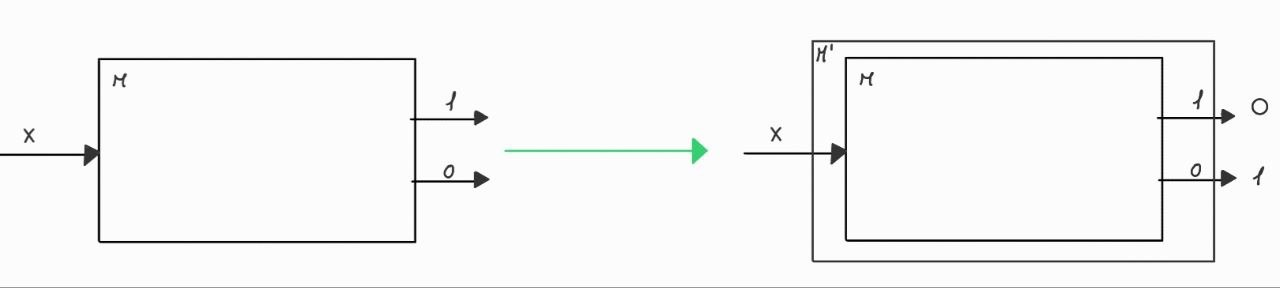
\includegraphics[width=0.5\textwidth]{img/MacchineTuring/dimostrazione1.png}
        \caption{Rappresentazione grafica della dimostrazione che il complemento
            di un linguaggio ricorsivo è ricorsivo}
    \end{figure}
\end{dimostrazione}
\begin{teorema}[\textbf{Linguaggio ricorsivo è anche ricorsivamente enumerabile}]
    Preso un linguaggio $L$ costruito alfabeto $\Sigma$ si ha che se
    $L \subseteq \Sigma^{\ast}$ se $L$ è ricorsivo è anche ricorsivamente
    enumerabile.
\end{teorema}
\begin{dimostrazione}
    Se $L$ è ricorsivo esiste una macchina di Turing che riconosce se, data una
    stringa $x$, tale che $x \in L$, rispondendo $1$ e risponde $0$ se $x \not\in
        L$.

    Costruisco ora una macchina di Turing $M'$ che se l'input $x$ non appartiene
    al linguaggio $L$, allora la macchina va in loop ($\perp$). Quindi, quando
    la macchina sta per rispondere con $0$, modifico la funzione di transizione
    $\delta$ per ottenere il loop, ottenendo una macchina che va in loop se
    $x \not\in L$, mentre restituisce $1$ se $x \in L$ e quindi $L$ è ricorsivamente
    enumerabile.
    \begin{figure}[!ht]
        \centering
        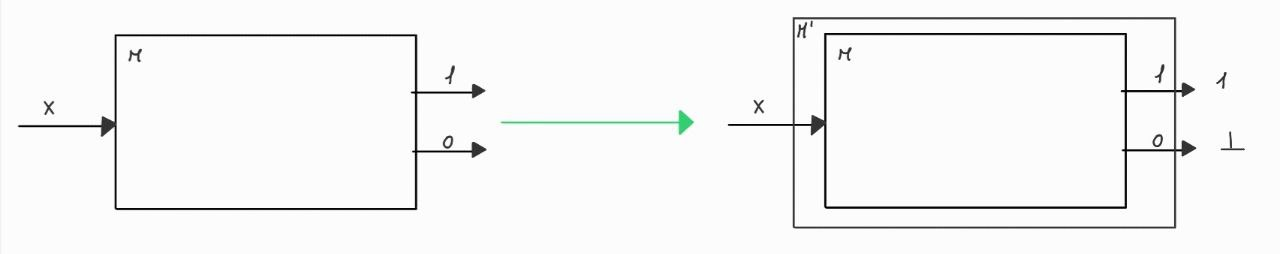
\includegraphics[width=0.5\textwidth]{img/MacchineTuring/dimostrazione2.png}
        \caption{Rappresentazione grafica della dimostrazione che un linguaggio
            ricorsivo è anche ricorsivamente enumerabile}
    \end{figure}
\end{dimostrazione}
\begin{teorema} \label{teo-rec-en-comp}
    $L$ è ricorsivo se e solo se $L$ è ricorsivamente enumerabile e il
    complementare di $L$, ossia $\overline{L}$, è ricorsivamente enumerabile.
\end{teorema}
\begin{dimostrazione}
    Rispetto alla dimostrazione precedente, che garantisce che se $L$ è ricorsivo
    allora è ricorsivamente enumerabile, devo definire, per il complementare,
    una macchina di Turing che va in loop se $x \in L$. Presa quindi una macchina
    di Turing $M$ che decide $L$, definisco $M'$ che accetta $L$, che quindi è
    ricorsivamente enumerabile. Definisco ora $M''$ che restituisce $1$ se
    $x \in \overline{L}$ ovvero $x \not\in L$ ed entra in loop se $x \not\in
        \overline{L}$, ovvero $x \in L$.

    Quindi $M$ decide $L$ eseguendo alternativamente $M'$ e $M''$ prestando
    attenzione alla gestione degli output.
\end{dimostrazione}
Vogliamo ora dimostrare che esistono dei problemi di decisione che non possono
essere risolti da una macchina di Turing. Per realizzare questa dimostrazione
partiamo da una nozione insiemistica: $|A| < |\mathcal{P}(A)|$, ovvero che la
cardinalità dell'insieme $A$ è sempre minore della cardinalità dell'insieme delle
parti di $A$ ($\mathcal{P}(A)$).

Con le informazioni ottenute in precedenza, abbiamo visto che possiamo
rappresentare una macchina di Turing partendo dall'alfabeto binario definito
come $B = \{0, 1\}$. Da questo, possiamo affermare che il numero di macchine di
Turing che possiamo realizzare sarà al più il numero di stringhe realizzabili
con l'utilizzo di $B$, ovvero $|B^{\ast}|$:
\begin{equation}
    |M| = |B^{\ast}|
\end{equation}
Inoltre, utilizzando l'alfabeto $B$, possiamo definire il linguaggio di
decisione come:
\begin{equation}
    L_D = \{x \in B^{\ast} \ | \ f_D(x) = 1\} \subseteq B^{\ast}
\end{equation}
quindi, possiamo affermare che il numero di problemi di decisione che si possono
avere è uguale a $|P(B^{\ast})|$. Partendo dal concetto insiemistico che è stato
definito in precedenza, possiamo affermare che:
\begin{equation}
    |M| = |B^{\ast}| < |P(B^{\ast})|
\end{equation}
ovvero che esistono problemi di decisione che \textbf{non posso} risolvere con
una macchina di Turing.
\subsection{Halting Problem}
Un esempio di problema di decisione che non può essere risolto da una macchina
di Turing è l'\textbf{halting problem}. Questo problema consiste nel determinare
se esiste un algoritmo che dati in input una macchina di Turing $M$ e una stringa
$x$, mi dica se la macchina $M$ eseguita sull'input $x$ termina.
\begin{definizione}[\textbf{Linguaggio associato all'Halting problem}]
    Posso definire formalmente l'\textbf{halting problem} con l'utilizzo del
    linguaggio $L_H$, definito come:
    \begin{equation}
        L_H = \{M \cdot \# \cdot x \ | \ M(x) \neq \perp \}
    \end{equation}
    ovvero come l'insieme di stringhe composte dalla descrizione di una macchina
    di Turing a cui è concatenato l'input tali per cui $M$ eseguita sull'input
    $x$ termina. Si utilizza il carattere $\#$ per separare la descrizione della
    macchina e l'input.
\end{definizione}
\begin{teorema}[\textbf{Halting problem non è decidibile}]
    Il linguaggio $L_H$ non è ricorsivo e quindi l'halting problem non è
    decidibile.
\end{teorema}
\begin{dimostrazione}[\textit{Per assurdo}]
    Assumiamo, per assurdo, che $L_H$ sia ricorsivo. Quindi esiste una macchina
    di Turing $M_H$ che prende in input $(M \cdot \# \cdot x)$ e mi fornisce in
    output:
    \begin{equation}
        M_H (M \cdot \# \cdot x) = \begin{cases}
            Y & \text{se} \ M(x) \ \neq \ \perp \\
            N & \text{se} \ M(x) \  = \ \perp
        \end{cases}
    \end{equation}
    Se esiste tale macchina, allora posso costruire una macchina di Turing $C$,
    costruita partendo da $M_H$ che prende in input $M$ e mi restituisce:
    \begin{equation}
        C(M) = \begin{cases}
            Y & \text{se} \ M_H(M, M) = N \\
            \perp & \text{se} \ M_H(M, M) = Y
        \end{cases}
    \end{equation}
    ovvero, se $M_H$ mi dice che $M$ su input $M$ non termina, allora $C$ termina
    in uno stato di accettazione, altrimenti, se $M_H$ mi dice che $M$ su input
    $M$ termina, allora $C$ restituisce $N$ e quindi non termina.

    A questo punto se fornisco alla macchina $C$ se stessa come input ottenendo
    due possibili situazioni:
    \begin{itemize}
        \item Se fornisco alla macchina $C$ se stesso come input, ovvero $C(C)$,
              e tale computazione termina in uno stato di accettazione ($C(C) = Y$),
              questo implica che la macchina $M_H$ eseguita su ($C, C$) entra in
              loop ($M_H(C, C) = N$). Quindi mi aspetto che la macchina $C$ non
              termini, ovvero $C(C) = \perp$ il che mi porta ad un assurdo.
        \item Al contrario, se $C(C) = \perp$, ovvero se la macchina $C$ eseguita su
              se stessa non termina, allora la macchina $M_H$ eseguita su ($C, C$)
              termina ($M_H(C, C) = Y$). Quindi mi aspetto che la macchina $C$
              termini, ovvero $C(C) \neq \perp$ il che mi porta ad un assurdo.
    \end{itemize}
    Posso quindi affermare che non esiste una macchina $M_H$ che decide $L_H$.
    \begin{figure}[!ht]
        \centering
        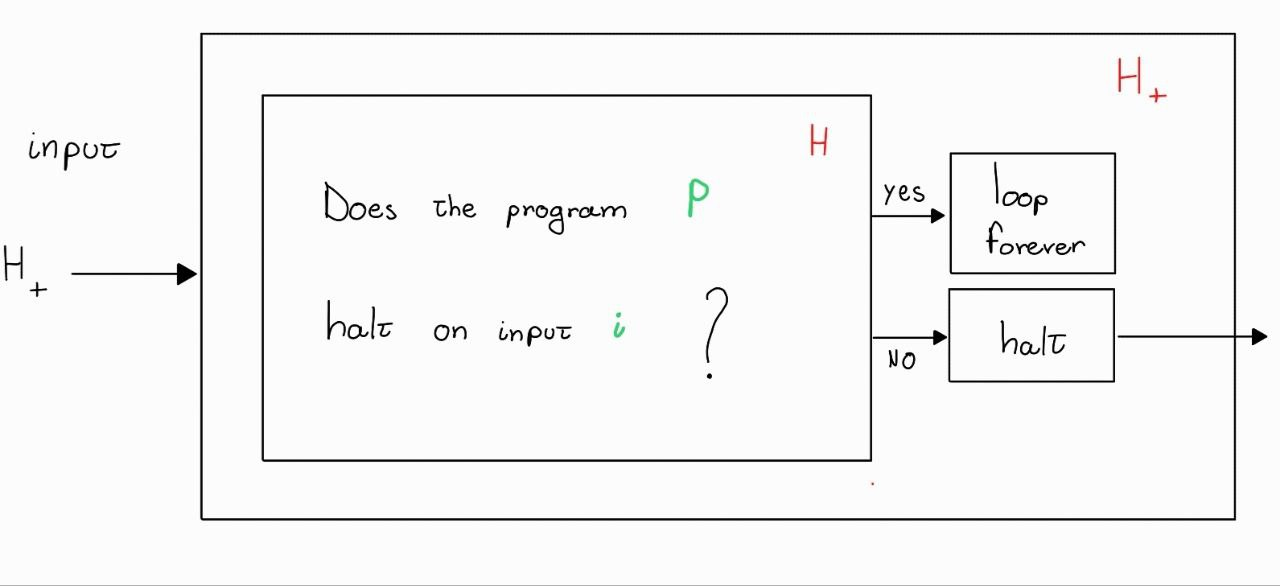
\includegraphics[width=0.5\textwidth]{img/MacchineTuring/halt.png}
        \caption{Rappresentazione grafica della dimostrazione dell'Halting problem}
    \end{figure}
\end{dimostrazione}
\begin{teorema}[\textbf{Halting problem è ricorsivamente enumerabile}] \label{teo-lh-rec-en}
    Il linguaggio $L_H$ è ricorsivamente enumerabile, ovvero il problema è
    parzialmente decidibile.
\end{teorema}
\begin{dimostrazione}
    Esiste una macchina di Turing $M_A$ che accetta il linguaggio $L_H$, ovvero
    tale che $M_A(M, x) = Y$ se e solo se $M(x) \neq \ \perp$.

    In precedenza abbiamo definito la macchina di Turing universale, la quale
    $U(M, x) = M(x)$, allora:
    \begin{equation}
        M_A(M, x) = \begin{cases}
            Y     & \text{se e solo se} \ U(M, x) = Y \ \lor \ N \\
            \perp & \text{se} \ U(M, x) = \perp
        \end{cases}
    \end{equation}
    Esiste quindi una macchina che accetta il linguaggio $L_H$.
\end{dimostrazione}
\begin{teorema}
    $\overline{L_H}$ non è ricorsivamente enumerabile.
\end{teorema}
\begin{dimostrazione} [\textit{Per assurdo}]
    Assumiamo per assurdo che $\overline{L_H}$ sia ricorsivamente enumerabile.
    Dal teorema \ref{teo-lh-rec-en} sappiamo che $L_H$ è ricorsivamente
    enumerabile, allora per quanto definito nel teorema \ref{teo-rec-en-comp} si
    ha che $L_H$ è ricorsivo, il che è assurdo in quanto è stato dimostrato che
    $L_H$ non è ricorsivo.
\end{dimostrazione}
\section{Problemi decidibili}
Vogliamo ora studiare i problemi decidibili classificandoli sulla base dei tempi
di esecuzione, considerando la dimensione dell'input e il caso peggiore. Per fare
questo utilizzeremo il tempo di esecuzione di una macchina di Turing. Questo
valore viene calcolato tramite il numero di passi che la macchina compie.
\begin{definizione}[\textbf{Tempo di calcolo}]
    Definiamo $t_M(x)$ come il \textbf{tempo di calcolo} di una macchina di
    Turing $M$ su input $x$. Non è il caso peggiore, ma dipendente dal singolo
    input specifico. Il tempo di calcolo è il numero di passi che esegue $M$ su
    input $x$ per dare una risposta.
\end{definizione}
Non si usa comunque il numero di passi nella realtà ma si usa la notazione
$\mathcal{O}$-grande, studiando il caso peggiore, ovvero il numero massimo di
passi.
\begin{definizione}[\textbf{Complessità temporale}]
    Definiamo $T_M(n)$ come la \textbf{funzione di complessità temporale} come:
    \begin{equation}
        T_M(n) = \max \{t_M(x) \ | \ |x| = n\}
    \end{equation}
\end{definizione}
\begin{definizione}[\textbf{Classe P}]
    Definisco la \textbf{classe $P$}in base alle macchine di Turing. La classe $P$ è
    definita come:
    \begin{equation}
        P = \{L \ | \ L \ \text{ è deciso da una macchina di Turing in tempo }
        \mathcal{O}(p(n))\}
    \end{equation}
\end{definizione}
\begin{definizione}[\textbf{Classe DTIME}]
    Definiamo la classe $DTIME(f(n))$ come la classe dei linguaggi decisi da una
    macchina di Turing entro un tempo $f(n)$:
    \begin{equation}
        DTIME(f(n)) = \{L \subseteq \Sigma^{\ast} \ | \ \exists M \
        \text{decide} \ L \ \text{in tempo} \ \mathcal{O}(f(n)) \}
    \end{equation}
    Quindi $DTIME(n)$ rappresenta l'insieme dei problemi di decisione che possono
    essere risolti con un algoritmo che lavora in tempo $\mathcal{O}(n)$. Quindi:
    \begin{equation}
        P = \bigcup_{c \in \mathbb{N}} DTIME(n^c)
    \end{equation}
    Infatti $P$ è l'unione di tutte le classi DTIME con funzioni polinomiali.
\end{definizione}
Possiamo dire che vale la seguente relazione tra le classi $DTIME$:
\begin{equation}
    DTIME(n) \subseteq DTIME(n^2) \subseteq DTIME(2^{n^c})
\end{equation}
Possiamo anche definire la classe \textbf{EXPTIME} come la classe di linguaggi
decidibili da una macchina di Turing in tempo esponenziale:
\begin{equation}
    EXPTIME =  \bigcup_{c \in \mathbb{N}} DTIME(2^{n^c})
\end{equation}
Inoltre, si ha che vale la seguente relazione tra le classi $P$ e $EXPTIME$:
\begin{equation}
    P \subseteq EXPTIME
\end{equation}
\begin{teorema}
    Se un problema è nella classe $P$ allora è risolvibile in un tempo efficiente.
\end{teorema}
Devo anche definire la complessità spaziale oltre a quella temporale.
\begin{definizione}[\textbf{Spazio}]
    Definisco lo \textbf{spazio} di calcolo $s_M(x)$ come il numero di celle del
    nastro usate dalla macchina di Turing $M$ con input $x$ durante la
    computazione.

    Il calcolo non è semplice come per il tempo, avendo anche decrementi. Quindi
    più che “celle usate” studiamo le “celle visitate”.
\end{definizione}
\begin{definizione}[\textbf{Complessità spaziale}]
    Definisco $S_M(n)$ come la \textbf{funzione di complessità spaziale}:
    \begin{equation}
        S_M(n) =  \max\{s_M(x) \ | \ |x| = n\}
    \end{equation}
\end{definizione}
Esiste una relazione tra la complessità spaziale e quella temporale per una
macchina di Turing. Se una computazione dura $n$ passi di tempo, allora posso
dire che al più ho usato $n$ celle di spazio, questo perché è possibile che in
alcune configurazioni la testina non si muove, ma nel caso peggiore si sposta
sempre. Si ha quindi:
\begin{equation}
    S_M(n) \leq T_M(n) + n
\end{equation}
con $+ \ n$ perché sul nastro abbiamo comunque l'input di lunghezza $n$.
\begin{teorema}
    Se il tempo è limitato allora lo spazio è limitato ma non vale l'opposto.
\end{teorema}
\begin{teorema}
    Se ho una macchina di Turing $M$ che lavora in spazio finito e tempo infinito,
    esiste una macchina di Turing $M'$ che fa la stessa cosa di $M$ in tempo
    limitato. Quindi se lo spazio è limitato allora il tempo è limitato.
\end{teorema}
\begin{dimostrazione}
    Infatti la macchina $M'$ può trovarsi in un numero finito di stati $k$ e
    avendo spazio limitato ho un numero limitato $S_M(n)$ di celle in cui si trova
    la testina. Ho anche un numero finito di simboli in alfabeto $\Sigma$ e quindi:
    \begin{equation}
        S_{M'}(n) \leq |k| \cdot |S_M(n)| \cdot |\Sigma|^{|S_M(n)|}
    \end{equation}
    avendo che prima o poi ritorno a stati già visti quindi la macchina se supera
    la quantità appena definita capisce di essere in loop. Quindi
    $|k| \cdot |S_M(n)| \cdot |\Sigma|^{|S_M(n)|}$ è anche un limite temporale
    per la seconda macchina.
\end{dimostrazione}
Quindi data una certa macchina che lavora in un certo spazio $S(n)$ posso costruire
una macchina equivalente che da la stessa risposta in tempo limitato $T(n)$. Si ha
che se ho un problema che si risolve in spazio polinomiale, per la formula appena
scritta avrò tempo esponenziale. Invece, al contrario, tempo polinomiale comporta
spazio polinomiale.
\section{Macchine di Turing non deterministiche}
Una \textbf{macchina di Turing non deterministica} si distingue da quella
deterministica nella funzione di transizione $\delta$. Nella macchina non
deterministica la funzione di transizione associa a ogni stato $q$ e a ogni
simbolo di nastro $X$ un \textit{insieme} di triple:
\begin{equation}
    \delta(q, X) = \{(q_1, Y_1, D_1), (q_2, Y_2, D_2), \dots, (q_k, Y_k, D_k)\}
\end{equation}
A ogni passo una macchina di Turing non deterministica sceglie una delle triple
come mossa, ovviamente lo stato, il simbolo di nastro e la direzione appartengono
alla stessa tripla. Nelle macchine non deterministiche la computazione non è una
sequenza di configurazioni ma un albero di computazione. Da ogni stato posso
passare a uno tra più stati, a seconda della scelta, formando così un albero. Il
singolo passo di computazione non è univocamente definito. Ogni singolo ramo
comunque è equivalente al passo di computazione della macchina di Turing
deterministica.
\begin{definizione}[\textbf{Linguaggio accettato}]
    Un linguaggio $L$ è \textbf{accettato} da una macchina di Turing non
    deterministica $N$ se per tutte le stringhe che fanno parte del linguaggio
    esiste almeno una computazione che termina nello stato $Y$, ovvero esiste
    una computazione per cui:
    \begin{equation}
        \forall x \in L \Rightarrow N(x) = Y
    \end{equation}
    Nel caso in cui nessuna delle computazioni termina nello stato $Y$, allora
    l'input non è accettato.
\end{definizione}
\begin{definizione}[\textbf{Linguaggio deciso}]
    Un linguaggio $L$ è \textbf{deciso} da una macchina di Turing non
    deterministica $N$ se, qualora la stringa $x$ appartenga il linguaggio,
    esiste almeno una computazione tale per cui:
    \begin{equation}
        x \in L \to N(x) = Y
    \end{equation}
    altrimenti, se $x$ non appartiene al linguaggio (\textbf{rifiuta}), per
    tutte le computazioni, si ha che:
    \begin{equation}
        x \not\in L \to N(x) = N
    \end{equation}
    Non devo quindi avere loop in questo caso, tutte devono dare $N$.
\end{definizione}
\begin{teorema}[\textbf{Equivalenza tra macchine di Turing deterministica e non
            deterministica}]
    Se $M_N$ è una macchina di Turing non deterministica, esiste una macchina di
    Turing deterministica $M_D$ tale che accettano gli stessi linguaggi $L(M_N)
        = L(M_D)$.
\end{teorema}
\begin{dimostrazione}
    La macchina di Turing deterministica $M_D$ può simulare la macchina di Turing
    non deterministica $M_N$ procedendo con una visita in ampiezza dell'albero
    di computazione. Viene eseguita una visita in ampiezza in modo da evitare di
    incappare in loop.
\end{dimostrazione}
La macchina di Turing non deterministica $N$ decide il linguaggio $L$ in tempo
$t_N(n)$, ovvero il tempo di calcolo è dato dall'altezza del ramo più lungo.
Come per le macchine deterministiche, definiamo $T_N(n)$ come:
\begin{equation}
    T_N(n) = \max \{t_N(x) \ | \ |x| = n\}
\end{equation}
Data una macchina di Turing non deterministica $N$ che decide $L$ in tempo
$T_N(n)$ esiste una macchina di Turing deterministica $M$ che decide $L$ in tempo
$2^{\mathcal{O}(T_N(n))}$. Questa complessità deriva dal fatto che se ogni nodo
dell'albero ha al massimo $b$ figli, allora l'albero di computazione ha al
massimo $b^{T_N(n)}$ foglie. Il numero interno di nodi è al massimo $b^{T_N(n)}
    - 1$ e quindi il numero totale di nodi è $< 2 \cdot b^{T_N(n)}$. Inoltre, un
cammino dalla radice alla foglia è $\mathcal{O}(T_N(n))$. Il tempo di esecuzione
della macchina $M$ è:
\begin{equation}
    \mathcal{O}(T(n) \cdot b^{T(n)}) = 2^{\mathcal{O}(T_N(n))}
\end{equation}
\begin{definizione}[\textbf{Classe NTIME}]
    Definiamo una funzione di tempo per una macchina di Turing non deterministica
    come:
    \begin{equation}
        NTIME(f(n)) = \{L \ | \ L \ \text{è deciso da una macchina di Turing non
            deterministica in tempo } \mathcal{O}(f(n))\}
    \end{equation}
\end{definizione}
Quest'ultima definizione ci permette di definire la classe di \textbf{problemi NP}
come l'insieme dei linguaggi $L$ che sono decisi in tempo polinomiale da una
macchina di Turing non deterministica:
\begin{equation}
    NP = \bigcup_{c \in \mathbb{N}} NTIME(n^c)
\end{equation}
\begin{osservazione}
    Sia $P$ l'insieme dei \textbf{problemi decidibili in tempo polinomiale} da
    una macchina di Turing deterministica, e $NP$ l'insieme dei \textbf{problemi
        decidibili in tempo polinomiale} da una macchina di Turing non
    deterministica. Sappiamo che è vero che $P \subseteq NP$ ma non è ancora
    dimostrato che $NP \subseteq P$.
\end{osservazione}
Possiamo però affermare che:
\begin{equation}
    P \subseteq NP \subseteq EXPTIME
\end{equation}
\subsection{Verificatori}
La classe $NP$ rappresenta una classe di linguaggi che sono verificabili in
tempo polinomiale da una macchina di Turing non deterministica. Verificare un
linguaggio significa che per ogni input $x \in L$ si ha una stringa $c$ detta
\textbf{certificato} che possiamo usare per verificare che effettivamente $x \in
    L$.
\begin{definizione}[\textbf{Verificatore}]
    Un \textbf{verificatore} di un linguaggio $L$ è una macchina di Turing
    deterministica $V$ tale per cui:
    \begin{equation}
        L = \{x | V \ \text{accetta} \ \langle x, c \rangle \
        \text{per qualunque stringa} \ c\}
    \end{equation}
    Questa macchina accetta le stringhe appartenenti al linguaggio eseguendo le
    istruzioni specificate dal certificato $c$.
\end{definizione}
Se $V$ richiede tempo polinomiale rispetto $x$ a per accettare/rifiutare, allora
$V$ è un verificatore in tempo polinomiale per $x$. Se esiste un verificatore in
tempo polinomiale per $L$, allora $L$ è verificabile in tempo polinomiale.

Dato che $V$ deve eseguire in tempo polinomiale rispetto a $x$, ne segue che $c$,
il certificato, deve essere di lunghezza polinomiale rispetto a $x$, altrimenti
non avremmo il tempo di leggere tutto $c$.

Supponiamo di avere una macchina di Turing non deterministica $M$ che lavora in
tempo polinomiale, costruiamo un verificatore $V$ che lavora in tempo polinomiale
per lo stesso linguaggio deciso da $M$. Se su input $x$ la macchina $M$ accetta,
significa che esiste una computazione accettante $C_1, \dots, C_k$ di lunghezza
polinomiale rispetto a $x$. Per ogni passaggio da $C_i$ a $C_{i + 1}$ è stata
applicata una transizione definita dalla funzione di transizione di $M$.

Usiamo come certificato $c$ la sequenza di transizioni applicate lungo tutta la
computazione, le quali sono in numero polinomiale. Queste transizioni ci
identificano una specifica computazione della macchina di Turing non
deterministica $M$. Il verificatore deve solo simulare quella computazione, senza
fare scelte non deterministiche, dato che le transizioni da fare sono tutte in
$c$ e verificare che la computazione accetti.

Abbiamo mostrato che per ogni linguaggio accettato da una macchina di Turing non
deterministica che lavora in tempo polinomiale possiamo costruire un verificatore
polinomiale per lo stesso linguaggio.

Dobbiamo mostrare ora l'inclusione in senso inverso. Sfruttiamo il fatto che
possiamo usare una macchina di Turing non deterministica per scrivere un
certificato sul nastro e, se esiste un certificato che ci permette di accettare,
questo sarà presente in una computazione.

Sia $V$ un verificatore in tempo polinomiale per $L$. Assumiamo $V$ esegua in
tempo $n^k$. Costruiamo una macchina di Turing non deterministica che su input
$x$ esegue due compiti:
\begin{itemize}
    \item Genera in modo non deterministico un certificato $c$ di lunghezza al
          più $n^k$.
    \item Simula $V$ su input $\langle x, c \rangle$ e accetta se $V$ accetta,
          mentre rifiuta se $V$ rifiuta.
\end{itemize}
Abbiamo mostrato che per ogni linguaggio per il quale esiste un verificatore
polinomiale possiamo costruire una macchina di Turing non deterministica che
decide lo stesso linguaggio in tempo polinomiale. Quindi le due definizioni di
$NP$ sono equivalenti.
\begin{esempio}[\textbf{Cammino Hamiltonian}]
    Consideriamo il problema del cammino Hamiltonian. Tale problema consiste nel
    dato un grafo orientato $G = (V, E)$ trovare trovare un cammino che visita
    tutti i nodi una sola volta. Consideriamo una variante in cui conosciamo il
    nodo di partenza $s$ e il nodo di arrivo $t$.
    \begin{equation}
        HAMPATH = \{\langle G, s, t \rangle \ | \ G \ \text{ha un cammino
            Hamiltonian da} \ s \ \text{a} \ t\}
    \end{equation}
    Per questo problema si può ottenere una semplice soluzione che lo risolve in
    tempo esponenziale, ovvero provare tutti i possibili cammini. Questa
    soluzione è però inefficiente.

    Questo problema ha una caratteristica chiamata \textit{verificabilità
        polinomiale}. Se in qualche modo si riesce a trovare un cammino
    Hamiltonian, allora possiamo verificare l'esistenza di tale cammino in tempo
    polinomiale.

    Per il problema del cammino Hamiltonian il certificato è rappresentato da
    un percorso Hamiltonian da $s$ a $t$. Il verificatore $V$ prende in input
    $\langle G, s, t, c \rangle$ e controlla che $c$ sia un cammino Hamiltonian
    da $s$ a $t$ in $G$. Per fare questo, il verificatore controlla che il primo
    nodo di $c$ sia $s$, che l'ultimo nodo sia $t$ e che ogni nodo di $c$ sia
    connesso al successivo.
    Da questo segue che il verificatore $V$ lavora in tempo polinomiale rispetto
    alla lunghezza del certificato $c$.
\end{esempio}
\subsection{Classi di problemi}
Definiamo ora altre classi di problemi:
\begin{itemize}
    \item \textbf{coP}: ovvero la classe di linguaggi di cui posso decidere la
          \textbf{non appartenenza} in tempo polinomiale:
          \begin{equation}
              coP = \{L \ | \ \overline{L} \in P\}
          \end{equation}
    \item \textbf{$\overline{P}$}: ovvero la classe di linguaggi che \textbf{non
              sono decidibili} in tempo polinomiale:
          \begin{equation}
              \overline{P} = \{L \ | \ L \not\in P\}
          \end{equation}
    \item \textbf{coNP}: ovvero la classe di linguaggi di cui posso decidere la
          \textbf{non appartenenza} in tempo polinomiale da una macchina di
          Turing non deterministica:
          \begin{equation}
              coNP = \{L \ | \ \overline{L} \in NP\}
          \end{equation}
\end{itemize}
\begin{nota}
    È importante notare che:
    \begin{equation}
        \overline{P} \neq coP
    \end{equation}
    \begin{equation}
        P \subseteq NP \ \land \ P \subseteq coNP \ \text{quindi} \ P
        \subseteq NP \cap coNP
    \end{equation}
\end{nota}
\begin{teorema}
    \begin{equation}
        P = coP
    \end{equation}
\end{teorema}
\begin{dimostrazione}
    Se un linguaggio $L \in P$, allora esiste una macchina di Turing
    deterministica che decide $L$ in tempo polinomiale:
    \begin{equation}
        \forall x \in \Sigma^{\ast} = \begin{cases}
            x \in L \Rightarrow M(x) = Y \\
            x \not\in L \Rightarrow M(x) = N
        \end{cases}
    \end{equation}
    Posso inoltre creare una macchina $M'$ che decide $\overline{L}$ in tempo
    polinomiale:
    \begin{equation}
        \forall x \in \Sigma^{\ast} = \begin{cases}
            x \in \overline{L} \Rightarrow M'(x) = Y \\
            x \not\in \overline{L} \Rightarrow M'(x) = N
        \end{cases}
    \end{equation}
    per ottenere questa macchina è sufficiente modificare gli stati di
    accettazione e rifiuto della macchina $M$.
\end{dimostrazione}
La dimostrazione precedente non può essere utilizzata per dimostrare che $NP =
    coNP$ dato che, nel caso di macchine non deterministiche è sufficiente che
esista un singolo ramo di computazione che termina in uno stato di accettazione.
Invertendo l'output di questa macchina si ottiene una macchina che non decide
$\bar{L}$ dato che sarebbero necessaire tutte computazioni che terminano in uno
stato accettante.
\section{Riduzioni polinomiali}
Le \textbf{riduzioni polinomiali} tra problemi, sono delle procedure che per ogni
istanza del problema $A$ la trasformano in un'istanza per un problema diverso $B$.
Quindi un'istanza di $A$, $I_A$, ha due risposte, $Y$ o $N$, ma posso passare
tramite una determinata funzione $f$, definita come:
\begin{equation}
    f: I_A \to I_B
\end{equation}
a un istanza $I_B$ tale che $B$ avrà risposte, uguali a quelle di $A$, $Y$ o $N$.
\begin{equation}
    \forall x \in I_A \ \begin{cases}
        A(x) = Y \Rightarrow B(f(x)) = Y \\
        A(x) = N \Rightarrow B(f(x)) = N
    \end{cases}
\end{equation}
In altre parole, si cerca una funzione $f$ che mi permette di convertire le
istanze del mio problema di partenza in istanze di un problema che so risolvere.
\begin{definizione}[\textbf{Riduzione polinomiale}]
    La \textbf{riducibilità polinomiale} tra problemi è definita come:
    \begin{equation}
        f: \Sigma^{\ast} \to \Sigma^{\ast}
    \end{equation}
    la quale deve essere calcolabile in tempo polinomiale da una macchina di
    Turing deterministica, tale che:
    \begin{equation}
        \forall x \in \Sigma^{\ast}, \ x \in L_A \ \text{se e solo se} \
        f(x) \in L_B
    \end{equation}
    Indichiamo l'operazione di riduzione polinomiale come:
    \begin{equation}
        L_A \leq_P L_B
    \end{equation}
\end{definizione}
\begin{osservazione}
    Si utilizza il simbolo minore uguale ($\leq$), per indicare una relazione
    d'ordine nella complessità dei problemi.
\end{osservazione}
\begin{teorema}
    Dato un linguaggio $L_A$ riducibile polinomialmente a $L_B$ ($L_A \leq_P L_B$),
    si ha che se $L_B \in P$ allora sicuramente anche $L_A \in P$.
\end{teorema}
\begin{dimostrazione}
    Infatti e esiste un algoritmo polinomiale per $L_B$ allora, avendo una
    trasformazione polinomiale ho che $f(x) + L_B$ è ancora polinomiale.
\end{dimostrazione}
\begin{teorema}[\textbf{Transitività}]
    La riduzione polinomiale gode della proprietà di transitività, ovvero:
    \begin{equation}
        L_A \ \leq_P \ L_B \ \land \ L_B \ \leq_P \ L_C \ \text{allora} \ L_A
        \ \leq_P \ L_C
    \end{equation}
    Posso ottenere questa riduzione applicando la composizione di funzioni.
\end{teorema}
\begin{definizione}[\textbf{NP-hard}]
    Un linguaggio $L$ è \textbf{NP}$\_$\textbf{hard} se vale che:
    \begin{equation}
        \forall L' \in NP \ \text{si ha} \ L' \leq_P L
    \end{equation}
\end{definizione}
\begin{definizione}[\textbf{NP-completo}]
    Un linguaggio $L$ si dice \textbf{NP}$\_$\textbf{completo} se valgono i
    seguenti punti:
    \begin{itemize}
        \item $L \in NP$
        \item $L \in NP\_hard$
    \end{itemize}
\end{definizione}
\begin{teorema}
    Se $L_A \leq_P L_B$ e $L_A \in NP\_hard$ allora so che anche $L_B \in NP\_hard$.
\end{teorema}
\begin{dimostrazione}
    Se $L_A \leq_P L_B$ per la definizione di $NP\_hard$ so che esistono n
    linguaggi che sono riducibili polinomialmente a $L_A$. Utilizzando la
    proprietà transitiva posso affermare che $L_B$ è $NP\_hard$.
\end{dimostrazione}
\begin{figure}[!ht]
    \centering
    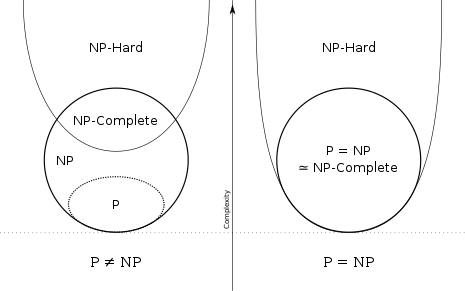
\includegraphics[width=0.5\textwidth]{img/MacchineTuring/classificazioneProblemi.png}
    \caption{Classificazione dei problemi.}
\end{figure}
\begin{teorema}[\textbf{Teorema Cook-Levin}]
    Il problema di soddisfacibilità SAT è \textbf{NP}$\_$\textbf{completo}.
    Questo problema prende in input una formula booleana $\phi$ in forma normale
    congiunta (CNF), ovvero che ha una congiunzione ($\land$) come legame tra le
    clausole. Una clausola è un $\lor$ di letterali, ovvero di variabili booleane
    $x_i$ o $\overline{x_i}$. In output ho se la forma sia soddisfacibile o meno.
\end{teorema}
\begin{dimostrazione}[\textit{Idea della dimostrazione}]
    Si ha che SAT può essere risolto in tempo esponenziale, $\mathcal{O}(2^n)$,
    provando tutti i possibili assegnamenti di verità possibili.

    Posso usare inoltre una macchina di Turing non deterministica che esegue
    tutti i rami in parallelo, con ogni possibilità di assegnamento fatta in un
    ramo oppure posso dire che “spara” un assegnamento a caso, che si suppone
    giusto, su un ramo e verifica che è giusto. In ogni caso con una macchina di
    Turing non deterministica avrei tempo polinomiale, $\mathcal{O}(n \cdot m)$
    per $n$ variabili e $m$ clausole.

    Per vedere che ogni problema $NP$, per semplicità decisionali, si riduce a SAT
    vedo che tutti i problemi in $NP$ hanno in comune di avere un macchina di
    Turing non deterministica che li risolve in tempo polinomiale, che decide il
    linguaggio associato. Basta quindi dire che $\forall \Pi ' \in  NP$ ha
    associato una macchina di Turing non deterministica $N'_{\Pi}$ che lavora in
    tempo polinomiale e mi basta vedere che ogni macchina di Turing non
    deterministica che lavora in tempo polinomiale si può trasformare in una
    formula CNF, presa in ingresso da SAT, sfruttando poi gli stati finali della
    computazione di SAT. Se SAT dice che è soddisfacibile allora lo è il problema
    iniziale e quindi il problema è riducibile a SAT.
\end{dimostrazione}
\begin{dimostrazione}[\textbf{Idea della dimostrazione}]
    Per dimostrare che SAT è $NP\_hard$ devo dimostrare che ogni problema in $NP$
    è riducibile polinomialmente a SAT. Per fare questo, dobbiamo costruire una
    riduzione polinomiale per ogni generico problema $\Pi \in NP$ a SAT. Tale
    riduzione prende in input una stringa $w$ e restituisce una formula booleana
    $\phi$ tale che:
    \begin{equation}
        w \in L_{\Pi} \iff \phi \in SAT
    \end{equation}
\end{dimostrazione}
\begin{dimostrazione}
    Per prima cosa dobbiamo verificare che $SAT$ sia in $NP$. Per fare questo
    dobbiamo costruire una macchina di Turing non deterministica che prova degli
    assegnamenti di verità e verifica che la formula sia soddisfacibile.

    A questo punto dobbiamo mostrare che ogni linguaggio $A$ in $NP$ è riducibile
    polinomialmente a $SAT$. Per fare ciò assumiamo di avere una macchina di
    Turing non deterministica $N$ che decide $A$ in tempo polinomiale ($n^k$).

    Definiamo ora una tabella, come quella riportata in figura \ref{fig:tab_levin_cook}, 
    per la macchina $N$ su input $w$ di dimensioni $n^k \times n^k$, dove le 
    righe sono le configurazioni di ogni ramo di computazione della macchina $N$ 
    su input $w$.
    \begin{figure}[!ht]
        \centering
        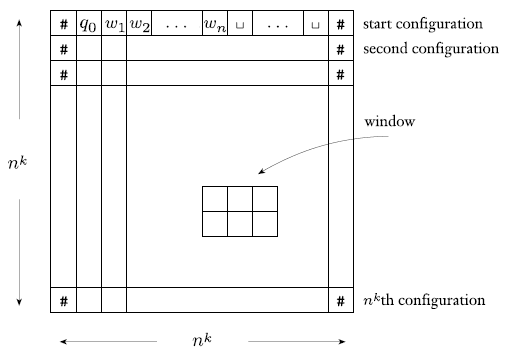
\includegraphics[width=0.5\textwidth]{img/MacchineTuring/tab_levin_cook.png}
        \caption{Tabella per la macchina $N$ su input $w$.}
        \label{fig:tab_levin_cook}
    \end{figure}

    Assumiamo per semplicità che ogni configurazione inizia e finisce con il simbolo $\#$.

    La prima riga della tabella è la configurazione iniziale di $N$ su input $w$, 
    mentre le successive sono calcolate dalla precedente in base alla funzione di
    transizione di $N$. Una tabella accetta se almeno una delle righe rappresenta 
    una computazione accettante di $N$ su input $w$.
\end{dimostrazione}
% https://en.wikipedia.org/wiki/Succinct_data_structure
\chapter{Strutture dati succinte}
Le \textbf{strutture dati succinte} sono una classe di strutture dati che forniscono
un compromesso tra l'efficienza dell'accesso ai dati e la quantità di spazio
utilizzato per memorizzare i dati. Queste strutture cercano di minimizzare l'uso
dello spazio di memoria, mantenendo nel contempo un accesso efficiente ai dati.

Le strutture dati succinte sono un tipo di struttura dati che utilizza una quantità
di spazio “vicina” al limite inferiore teorico dell'informazione, ma che, a
differenza di altre rappresentazioni compresse, consente ancora operazioni di
interrogazione efficienti.

Supponiamo che $\mathcal{Z}$ sia il numero ottimale teorico di bit necessari per
memorizzare alcuni dati. Una rappresentazione di questi dati viene chiamata:
\begin{itemize}
    \item \textbf{Implicita} se richiede $\mathcal{Z} + \mathcal{O}(1)$ bit di
          spazio. (es. $\mathcal{Z} + 14$ bit)
    \item \textbf{Succinta} se richiede $\mathcal{Z} + o(\mathcal{Z})$ bit di spazio.
          (es. $\mathcal{Z} + \log \mathcal{Z}$ oppure $\mathcal{Z} + \sqrt{
                  \mathcal{Z}}$ bit)
    \item \textbf{Compatta} se richiede $\mathcal{O}(\mathcal{Z})$ bit di spazio.
          (es. $5 \cdot \mathcal{Z}$ bit)
\end{itemize}
\begin{nota}
    $o(\mathcal{Z})$ si riferisce al concetto matematico di \textit{o-piccolo},
    ovvero:
    \begin{equation}
        \lim_{x \to x_0} \frac{f(x)}{g(x)} = 0 \Rightarrow f(x) = o_{x_0} (g(x))
        \ \text{con} \ x_0 = + \infty
    \end{equation}
\end{nota}
\section{Bitvector}
Un modo di rappresentare le strutture dati succinte è attraverso l'utilizzo di
\textbf{bitvector}.
\begin{definizione}[\textbf{Bitvector}]
    Si definisce un \textbf{bitvector} $B$ come un array di lunghezza $n$, popolato
    da elementi binari ($\{0, 1\}$). Formalmente si ha:
    \begin{equation}
        B[i] \in \{0, 1\}, \ \forall i \ \text{tale che} \ 1 \leq i \leq n
    \end{equation}
    In alternativa all'alfabeto binario è possibile utilizzare i valori booleani
    vero e falso ($\{\top, \bot\}$).
\end{definizione}
Su questa struttura è possibile effettuare due operazioni:
\begin{itemize}
    \item \textbf{rank}: restituisce il numero di elementi uguali a $q$ che sono
          presenti nella struttura dati fino a $x$.
          \begin{equation}
              rank_q(x) = \sum_{k = 1}^{k \leq i} B[k], \ \forall i \
              \text{tale che} \ 1 \leq i \leq n \ \land \ B[k] = q
          \end{equation}
    \item \textbf{select}: restituisce la posizione della $x$-esima occorrenza
          di $q$.
          \begin{equation}
              select_q(x) = \min{\{k \in [0, \dots, n): \ rank_q(k) = x\}}
          \end{equation}
\end{itemize}
\begin{nota}
    \begin{equation}
        rank_q(select_q(i)) = i
    \end{equation}
\end{nota}
È possibile ottenere una struttura dati succinta, usando $o(n)$ bit aggiuntivi,
che permetta di effettuare le operazioni di \textit{rank} e \textit{select} in
tempo costante $\mathcal{O}(1)$.
\subsection{Funzione rank}
Vediamo ora come è possibile rendere il tempo di esecuzione dell'operazione di
rank costante ($\mathcal{O}(1)$).

La soluzione più semplice, ovvero memorizzare tutti i valori di $rank(i)$
necessiterebbe di $\mathcal{O}(n \log n)$ bit il che non lo rende un o-piccolo
di $n$. Una soluzione alternativa consiste nel memorizzare ogni $l-$esimo valore
$rank(i)$, e a questo punto, quando si esegue una query scorriamo i restanti $l
    - 1$ bit.

Questi valori vengono salvati in un vettore \textit{first} $F[0 \dots n / l]$,
dove l'operatore $/$ indica la divisione intera, tale che:
\begin{itemize}
    \item $F[0] = 0$
    \item $F[i / l] = rank(i)$ se $i \mod l = 0$
\end{itemize}
Se $l = \left(\left\lceil \frac{\log n}{2} \right\rceil \right)^2$ si ha un ordine
di $\frac{n}{\log n}$ bit per l'array $F$. Con questa prima operazione è possibile
eseguire una rank come:
\begin{equation}
    rank(i) = F[i/l] + C(B[l \cdot (i / l) + 1 \dots i])
\end{equation}
con $C(B')$ che rappresenta una funzione che conta i simboli $\sigma = 1$ in $B'$.
Questa soluzione mi porta a una rank eseguita in tempo $\mathcal{O}(\log^2 n)$.

Aumentando la quantità di informazioni salvate in memoria, possiamo ridurre
ulteriormente il tempo di esecuzione della funzione di rank.

Nello specifico, in ogni blocco di lunghezza $l$, indotto da $F$, memorizziamo
ogni $k$ posizioni il numero di simboli $\sigma = 1$ a partire dall'inizio del
blocco, escludendo la posizione iniziale in cui il valore di rank è già in $F$.
Otteniamo un vettore \textit{second} $S[0 \dots l /k]$ dove:
\begin{itemize}
    \item $S[i / k] = 0$ se $k \mod l = 0$
    \item $S[i / k] = rank_{B[l \cdot (i / l) + 1 \dots i]} (i - l \cdot (i / l)
              + 1)$ se $i \mod k = 0$
\end{itemize}
Questa soluzione richiede $\mathcal{O}\left(\left(\frac{n}{k}\right) \log l\right)$
bit aggiuntivi. In particolare, scegliendo $k = \left\lceil \frac{\log n}{2}
    \right\rceil$ si ottiene uno spazio di $\mathcal{O}(\frac{n \log \log n}{\log n})$
bit. Introducendo questo secondo vettore è possibile eseguire una rank come:
\begin{equation}
    rank(i) = F[i / l] + S[i / k] + C(B[k \cdot (i / k) + 1 \dots i])
\end{equation}
Questa soluzione mi porta a una rank eseguita in tempo $\mathcal{O}(\log n)$.

Per ottenere una rank in tempo costante si utilizza la tecnica \textbf{Four
    Russians technique}. Questa tecnica consiste nel salvare una look-up table
third $T$, di dimensioni $2^{k - 1} \times k - 1$, i valori di $rank(i')$
per tutte le posizioni $k - 1$, in tutte le possibili configurazioni indotte dai
blocchi definiti per $S$. Così facendo la lookup-table $T$ richiede uno spazio
per essere memorizzata pari a $\mathcal{O}(\sqrt{n} \log n \log \log n)$ bit.

Si definisce:
\begin{equation}
    c_i = B \left[k \cdot \left(\frac{i}{k}\right) + 1 \dots k \cdot \left(\frac{i}{k} 
    + 1\right) - 1\right]
\end{equation}
come il bitvector di lunghezza $k - 1$ che copre il $(k + 1)-$esimo blocco. Questo
valore ci permette di identificare la riga della lookup table $T$ da cui prendere
il valore di $rank(i)$. Mentre la colonna si ottiene da $i \mod k$. In questo
modo è possibile eseguire una rank in tempo costante $\mathcal{O}(1)$.
\begin{equation}
    rank(B) = \begin{cases}
        F[i/l]                                   & \text{se} \ i \mod l = 0    \\
        F[i/l] + S[i/k]                          & \text{se} \ i \mod l \neq 0
        \land i \mod k = 0                                                     \\
        F[i/l] + S[i/k] + T[c_i][(i \mod k) - 1] & \text{se} \ i \mod l \neq 0
        \land i \mod k \neq 0                                                  \\
    \end{cases}
\end{equation}
Così facendo, memorizzando un $o(n)$ bit in aggiunta alla struttura, posso
eseguire l'operazione di rank in tempo costante.
\begin{nota}
    Le operazioni per arrivare alla costruzione delle struttura dati che mi
    permette di eseguire la rank in tempo costante sono eseguite in tempo lineare
    ($\mathcal{O}(n)$).
\end{nota}
\begin{esempio}
    Vediamo un esempio di come può essere implementata la funzione rank in modo
    da effettuare accesso in tempo costante. Consideriamo il bitvector
    $B = 100101010010$ e scegliamo i valori di $l = 9$ e $k = 3$. Per eseguire
    la funzione rank in tempo costante si ottiene la struttura riportata in
    figura \ref{fig:rank}.
    \begin{figure}[!ht]
        \centering
        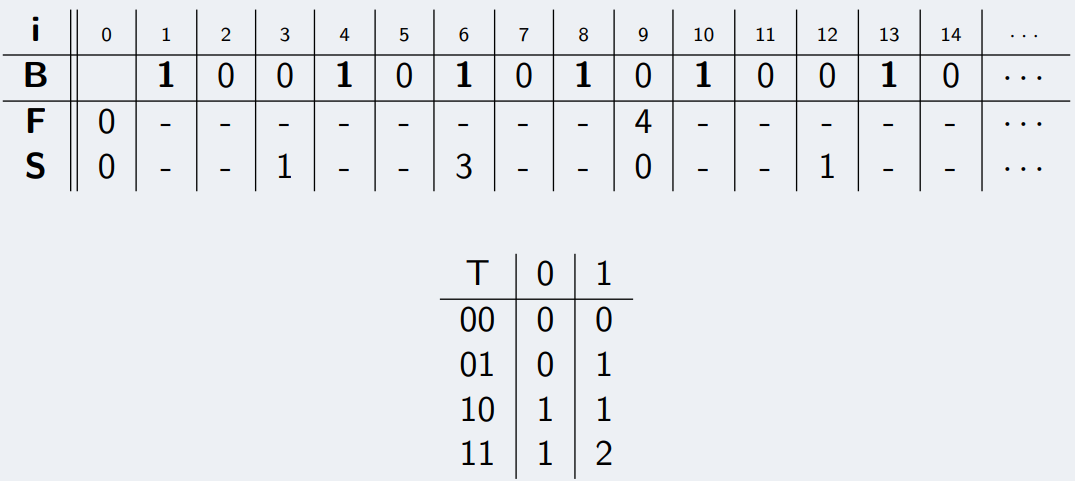
\includegraphics[width=0.5\textwidth]{img/Strutture Dati/rank.png}
        \caption{Esempio di implementazione della funzione rank}
        \label{fig:rank}
    \end{figure}
\end{esempio}
\begin{osservazione}
    Si può dimostrare che, con un procedimento abbastanza analogo a quello visto
    per la funzione di rank, è possibile costruire una struttura che necessita di
    $o(n)$ bit aggiuntivi e che permette di effettuare l'operazione di select in
    tempo costante.
\end{osservazione}
\section{Level Order Unary Degree Sequence}
Consideriamo in memoria la rappresentazione di un albero etichettato con $n$ nodi.
La classica rappresentazione attraverso puntatori richiede uno spazio pari a
$\mathcal{O}(n \log n)$.

Analizziamo ora una rappresentazione basata sulla visita in left-to-right
level-order di un albero, ovvero una visita in ampiezza. Utilizzando questa
visita, si salva per ogni nodo il suo grado e si memorizza la sequenza dei gradi
$D$ attraverso un prefix code binario. Quindi, per ogni nodo si aggiunge a un
bitvector $B$ i simboli della sequenza $1^d0$, con $d$ che rappresenta il grado.

In questa rappresentazione si considera un nodo detto \textbf{super-root}, il
quale viene aggiunto in modo che il numero di valori uguali a 1 presenti nel
bitvector sia uguale al numero di nodi dell'albero.

In questo modo si arriva a ottenere un bitvector di lunghezza $2n + 1$ dove si
ha un simbolo 1 associato a ogni nodo dell'albero. Con questa rappresentazione
posso indicare il nodo $m$ con l'indice relativo del corrispondente bit 1.

Utilizzando le operazioni rank e select definite per il bitvector, è possibile
implementare un set di operazioni per interrogare questa rappresentazione
dell'albero.
\begin{itemize}
    \item $is\_leaf(v) = T$ se e solo se $select_0(v) = select_0(v + 1) - 1$ in
          quanto per costruzione una foglia aggiunge solo uno 0 al bitvector $B$,
          quindi con $select_0(v)$ troviamo la posizione dello 0 posto in $B$ dal
          nodo antecedente a $v$ nella visita (quello antecedente perché abbiamo
          il 10 della super-root) e con $select_0(v + 1)$ la posizione dello 0
          relativo a $v$. Se sono in due posizioni adiacenti significa che $v$ ha
          aggiunto solo uno $0$ e quindi è una foglia.
    \item $first\_child(v) = rank_1(select_0(rank_1(select_1(v)))+1) = rank_1
              (select_0(v)+1)$:
          \begin{itemize}
              \item $k = select_0(v) + 1$ restituisce la posizione $k$ su $B$ del
                    primo "figlio" di $v$. In altri termini il $v$-esimo 0 mi
                    dice che ho finito di "visitare" la sotto-sequenza di bitvector
                    costruita per il nodo $v - 1$ e al bit successivo inizia la
                    sequenza del bitvector per $v$.
              \item $m = rank_1(k)$ restituisce il numero di nodo dell'albero in
                    posizione $k$ di $B$, quindi la label del primo "figlio" di
                    $v$.
              \item Imponiamo che $first\_child(v) = - 1$ se $is\_leaf (v) = T$
          \end{itemize}
    \item $last\_child(v) = rank_1(select_0(rank_1(select_1(v))+1)-1) = rank_1
              (select_0(v+1)-1)$:
          \begin{itemize}
              \item $k = select_0(v + 1)$ restituisce la posizione $k$ su $B$
                    dello $0$ inserito in visita level-order del nodo con label
                    $v$. In altri termini, il (v + 1)-esimo 0 mi dice che ho
                    finito di "visitare" la sotto-sequenza di bitvector costruita
                    per il nodo $v$.
              \item $w = k - 1$ restituisce l'indice dell'ultimo 1 inserito in
                    visita level-order del nodo con label j, quindi l'indice su
                    B dell'ultimo "figlio" di c. In altri termini, con la
                    precedente operazione si raggiunge lo 0 di $1^d 0$ e col -1
                    l'ultimo 1 di $1^d$
              \item $m = rank_1(w)$ restituisce il numero di nodo dell'albero in
                    posizione $w$ di B, quindi la label dell'ultimo "figlio" di v.
              \item Imponiamo che $last\_child(v) = -1$ se $is\_leaf (v) = T$
          \end{itemize}
    \item $parent(v) = rank_1(select_1(rank_0(select_1(v)))) = rank_0(select_1(v))$:
          \begin{itemize}
              \item $i = select_1(v)$ restituisce la posizione $i$ del nodo $v$
                    nel bitvector $B$ (identificando in quale $1^d 0$ è stato
                    aggiunto).
              \item $j = rank_0(i)$ restituisce il numero di sequenze che sono
                    state aggiunte al bitvector $B$ fino a quella relativa al
                    "genitore" del nodo in posizione $i$. Il numero di tali
                    sequenza è l'indice del nodo "genitore" per definizione di
                    vista level order e conseguente etichettatura dei nodi.
              \item Imponiamo che $parent(v) = -1$ se $v = 1$ (non considero la
                    super-root)
          \end{itemize}
    \item $degree(v) \ = \ last\_child(v) - first\_child(v) + 1$, imponiamo 
          $degree(v) = 0$ se $last\_child(v) = first\_child(v) = -1$
    \item $nth\_child(v, nth) = rank_1(select_1(first\_child(v)) + nth - 1)$,
          imponiamo $nth\_child(v, nth) = -1$ se $degree(v) < nth$
\end{itemize}
\begin{esempio}
    In figura \ref{fig:louds}, è riportata la costruzione di un e Level Order
    Unary Degree Sequence.
    \begin{figure}[!ht]
        \centering
        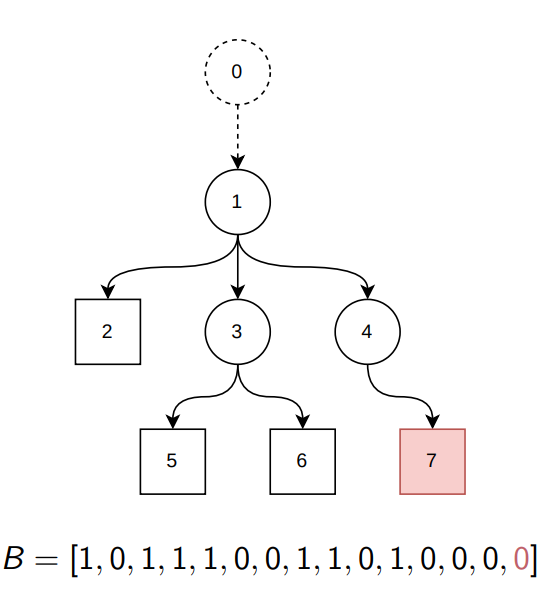
\includegraphics[width=0.5\textwidth]{img/Strutture Dati/LOUDS.png}
        \caption{Esempio di costruzione di un e Level Order Unary Degree Sequence}
        \label{fig:louds}
    \end{figure}
\end{esempio}
\section{Wavelet Tree}
Abbiamo visto come rank e select possono essere usati per interrogare un bitvector,
che ha un alfabeto fisso di grandezza 2. Siamo ora interessati a generalizzare
tali query ad un alfabeto di grandezza arbitraria. Per praticità assumiamo di
avere un alfabeto $\Sigma = [1 \dots s]$ il quale è ordinato nel seguente modo:
\begin{equation}
    \Sigma[i] \prec \Sigma[j] \iff i < j \dots
\end{equation}
Dato un generico alfabeto $\Sigma$ e una sequenza $T[1\dots n] \in \Sigma$ possiamo
ri-definire le funzioni di rank e select come:
\begin{itemize}
    \item $rank_{\sigma,T} (i)$ conta tutte le occorrenze del simbolo $\sigma
              \in \Sigma$ fino all'indice $i$ in $T$, $i \leq | T |$.
    \item $select_{\sigma,T} (i)$ ritorna la posizione dell'i-esima occorrenza
          del simbolo $\sigma \in \Sigma$ in $T$, $i \leq | T |$.
\end{itemize}
\begin{equation}
    rank_{\sigma,T} (select_{\sigma,T} (i)) = i, \ \forall \sigma \in \Sigma
    \land \forall i = 1 \dots n
\end{equation}
Una rappresentazione ``naïve'' consiste nel considerare come rappresentazione di
$T$ attraverso un insieme di $s$ ($| \Sigma | = s$) stringhe binarie $B_\sigma[1
        \dots n]$, $\forall \sigma \in \Sigma$, ovvero una per ogni simbolo
dell'alfabeto, si ha che:
\begin{equation}
    B_\sigma[i] = \begin{cases}
        1 \iff T[i] = \sigma \\
        0 \iff T[i] \neq \sigma
    \end{cases}
\end{equation}
Se per ogni bitvector $B_\sigma$ abbiamo calcolato la struttura a supporto vista
precedentemente si ha $rank_{\sigma,T} (i)$ in tempo costante $\mathcal{O}(1)$ e
uno spazio pari a $s \cdot (n + o(n))$ bit aggiuntivi.

Possiamo ottenere una rappresentazione più efficiente in memoria senza sacrificare
troppo i tempi di query. Per realizzare questa rappresentazione consideriamo un
\textbf{albero binario perfettamente bilanciato} dove ogni nodo corrisponde ad un
sottoinsieme di $\Sigma$.

I due figli di ogni nodo partizionano il corrispondente sottoinsieme di $\Sigma$
in due. A ogni nodo $v$ corrisponde una sequenza chiamata $R_v$, la quale è una
sotto-sequenza dell'input $T$ ed è anche una sotto-sequenza della sequenza con
cui è etichettato il nodo genitore di $v$. La root corrisponde alla sequenza $R_v = T$.

A ogni nodo $v$ si associa un bitvector, denotato con $B_v$, che indica a quale
dei due figli del nodo $v$ ogni simbolo della sotto-sequenza $R_v$ appartiene.

Se consideriamo l'indice $j$, con $1 \leq j \leq |R_v|$, abbiamo che:
\begin{itemize}
    \item Se $B_v [j] = 0$, allora il carattere associato $R_v [j]$ appartiene
          alla sotto-sequenza rappresentata dal figlio di sinistra.
    \item Se $B_v [j] = 1$, allora il carattere associato a $R_v [j]$ appartiene
          alla sotto-sequenza rappresentata dal figlio di destra.
\end{itemize}
Le foglie dell'albero sono \textit{virtualmente} etichettate con i singoli
caratteri dell'alfabeto. In realtà ci basta la funzione $rank_1$ eseguita sui
bitvector che etichettano i genitori delle foglie per recuperare l'informazione.
\subsection{Operazioni}
Vediamo ora come realizzare le operazioni su questa struttura dati:
\begin{itemize}
    \item \textbf{rank}: il calcolo dell'operazione rank inizia nel nodo root,
          nel quale si determina a quale dei due figli appartiene $\sigma$.
          Questa operazione avviene utilizzando l'ordinamento dell'alfabeto. In
          particolare, nella radice se $B_v [j] = 0$ allora $R_v [j] = \Sigma
              \left[\left\lceil \frac{s}{2} \right\rceil\right] \lor R_v [j]
              \prec \Sigma \left[\left\lceil \frac{s}{2} \right\rceil\right]$,
          ovvero il carattere si trova nella prima metà dell'alfabeto. Altrimenti
          se $B_v[j] = 1$ allora il carattere che si cerca è nella seconda metà
          dell'alfabeto.

          A questo punto si prosegue nel seguente modo fino a raggiungere le foglie:
          \begin{itemize}
              \item Se $\sigma = \Sigma\left[\left\lceil \frac{s}{2} \right\rceil
                            \right] \lor \sigma \prec \Sigma\left[\left\lceil
                            \frac{s}{2} \right\rceil\right]$ (siamo nella prima
                    metà dell'alfabeto indotto dal nodo), allora si prosegue
                    verso il figlio di sinistra, aggiornando il valore di $i$ con
                    $i = rank_{0,B_v}(i)$.
              \item Altrimenti, ovvero se siamo nella seconda metà, usiamo il
                    figlio di destra, e aggiorniamo il valore di $i$ con $i =
                        rank_{1,B_v}(i)$.
          \end{itemize}
          Nel nuovo nodo $v$ si procede nello stesso modo, considerando che ora
          $\Sigma = \Sigma \left[1 \dots \left\lceil \frac{s}{2} \right\rceil\right]$
          se si è andati a sinistra e $\Sigma = \Sigma\left[\left\lceil
                  \frac{s}{2} \right\rceil + 1 \dots s\right]$ se si è andati a
          destra.

          Si prosegue fino ad una foglia e $rank_{\sigma,T} (i) = i'$, dove $i'$
          è l'ultimo valore di i che si ottiene nei vari step.

          L'albero ha altezza $\lceil \log s\rceil$ quindi $rank_{\sigma,T} (i)$
          può essere calcolato in $\mathcal{O}(\log s)$, dove $s$ è la cardinalità
          dell'alfabeto.
    \item \textbf{random access}: in questo caso la scelta del figlio dipende
          unicamente da $B_v [i]$:
          \begin{itemize}
              \item Se $B_v [i] = 0$ proseguo verso il "figlio" di sinistra,
                    con $i = rank_{0,B_v}(i)$
              \item Se $B_v [i] = 1$ proseguo verso il "figlio" di destra,
                    con $i = rank_{1,B_v}(i)$
          \end{itemize}
          Si prosegue fino ad una foglia scegliendo il percorso da seguire in
          base al valore di $B_v [i]$.

          $T[i]$ è il simbolo che etichetta la foglia raggiunta alla fine della
          visita dato che il wavelet tree di una sequenza $T$ garantisce random
          access alla sequenza stessa possiamo sostituirla col suo wavelet tree.

          L'albero ha altezza $\lceil\log s \rceil$ quindi $access_{\sigma,T} (i)$
          può essere calcolato in $\mathcal{O}(\log s)$.
    \item \textbf{select}: analogamente ai bitvector si può dimostrare che anche
          $select_{\sigma,T}(i)$ può essere calcolato in $\mathcal{O}(\log s)$
\end{itemize}
\begin{nota}
    Nell'operazione di access ad ogni passo si effettua l'operazione di rank
    in base al valore del bit $B_v [i]$. Quindi per ogni nodo si effettua una
    scelta se effettuare una rank sul valore $0$ o sul valore $1$.
\end{nota}
\subsection{Costruzione}
Vediamo ora come costruire un wavelet tree livello per livello a partire dalla
root:
\begin{enumerate}
    \item Si etichetta la root con $R_v = T$ e un bitvector $B_v$ tale che
          $\forall i$, con $1 \leq i \leq |T|$:
          \begin{equation}
              B_v[i] = \begin{cases}
                  0 \iff T[i] = \Sigma\left[\left\lceil \frac{s}{2}
                      \right\rceil\right] \lor T[i] \prec \Sigma\left[
                  \left\lceil \frac{s}{2} \right\rceil\right] \\
                  1 \text{ altrimenti}
              \end{cases}
          \end{equation}
    \item Si estrae la sotto-sequenza $T'$ corrispondente ai valori 0 di $B_v$ e
          la si usa per etichettare il ``figlio'' di sinistra $v_1$ (che è relativo
          all'alfabeto $\Sigma = \Sigma\left[1 \dots \left\lceil \frac{s}{2}
                  \right\rceil\right]$) mentre quella corrispondente ai valori 1
          la si usa per etichettare il ``figlio'' di destra $v_2$ (che è relativo
          all'alfabeto $\Sigma = \Sigma\left[\left\lceil \frac{s}{2} \right\rceil
                  + 1 \dots s \right]$) per entrambe.
    \item Posso quindi cancellare $T$ e costruire i bitvector $B_{v1}$ e $B_{v2}$,
          con le rispettive strutture per la funzione rank e continuare
          ricorsivamente fino al raggiungimento delle foglie (quando si
          raggiungono alfabeti di cardinalità 1).
\end{enumerate}
Il processo di costruzione di un wavelet tree richiede un tempo pari a
$\mathcal{O}(n \log s)$.

In ogni momento della costruzione del wavelet tree abbiamo un bound in spazio
pari a $3n \log s + \mathcal{O}(s \log n)$, dato da:
\begin{itemize}
    \item 3 sotto-sequenze di $T$, quella del "genitore" e quelle dei due "figli".
    \item Tutti i bitvector finora computati che formano il wavelet tree.
    \item I puntatori che memorizzano la struttura ad albero.
\end{itemize}
Un ulteriore miglioramento in spazio si può ottenere concatenando tutti i bitvector
in un unico bitvector con una sola struttura a supporto della funzione rank. In
tal caso la struttura ad albero si può inferire dai partizionamenti dell'alfabeto
e dai bitvector. Questa variante è chiamata \textbf{levelwise wavelet tree}.

Un wavelet tree per una sequenza lunga $n$ costruita su alfabeto di cardinalità
$s$ occupa, avendo $\mathcal{O}(s \log n)$ per la topologia dell'albero:
\begin{equation}
    n \log s + o(n \log s) + \mathcal{O}(s \log n) \ bit
\end{equation}
Mentre, un levelwise wavelet tree richiede:
\begin{equation}
    n \log s + o(n \log s) \ bit
\end{equation}
\begin{esempio}
    Costruzione di un wavelet tree:
    \begin{figure}[!ht]
        \centering
        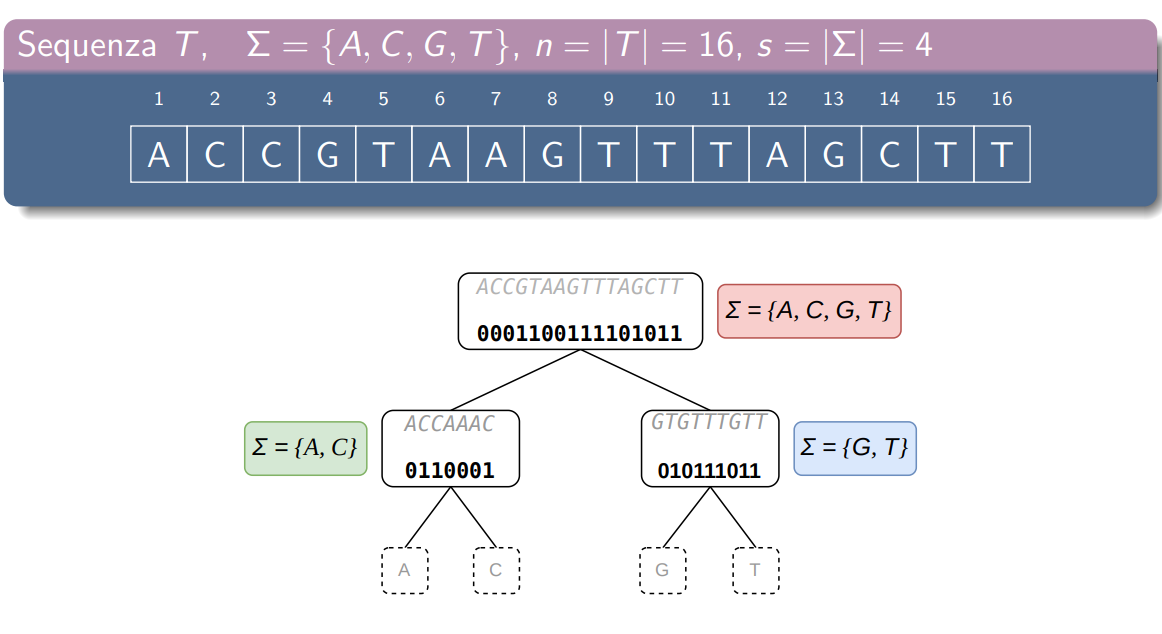
\includegraphics[width=0.5\textwidth]{img/Strutture Dati/wavelet tree.png}
        \caption{Esempio di costruzione di un wavelet tree su una sequenza semplice}
    \end{figure}
\end{esempio}
\section{Altre strutture dati succinte}
\begin{itemize}
    \item \textbf{Parentesi bilanciate}: si costruisce a partire dalla DFS
          dell'albero (preorder):
          \begin{itemize}
              \item ``('' quando si raggiunge un nodo per la prima volta.
              \item ``)'' quando si è terminata la visita del sotto-albero.
          \end{itemize}
    \item Strutture dati succinte che supportano le \textbf{range minimum queries}.
    \item \textbf{Wavelet matrix}: nascono con l'idea di migliorare i levelwise
          wavelet tree nella gestione di larghi alfabeti:
          \begin{itemize}
              \item tempi di access dimezzati
              \item tempi di rank e select leggermente ridotti
          \end{itemize}

          L'idea è che i bit di un nodo "figlio" non sono più "allineati" al
          "genitore" ma si assume che passando da un livello all'altro, tutti gli
          zero vanno da una parte e gli uni dall'altra.

          Salvando ad ogni livello $l$ il numero totale di simboli $\sigma = 0$
          $z_l$, richiedendo in totale $\mathcal{O}(\log n \log s)$ bit, si ottiene
          lo stesso comportamento di un levelwise wavelet tree.

          Una wavelet matrix richiede $n \log s + o(n \log s)$ bit, può essere
          costruita in $\mathcal{O}(n \log s)$ e risponde alle stesse query di un
          (levelwise) wavelet tree in $\mathcal{O}(\log s)$
\end{itemize}
\begin{definizione}[\textbf{Range Minimum Query}]
    Dato un array $A[1\dots n]$ di numeri $n$ elementi da un universo totalmente
    ordinato la \textbf{Range Minimum Query} $RMQ_A(i, j)$, con $1 \leq i \leq
        j \leq n$, restituisce la posizione $k$ di un elemento minimo in $A[i
                \dots j]$:$$RMQ_A(i, j) = argmin_{i \leq k \leq j}\{A[k]\}$$

    Si può dimostrare che è possibile costruire una struttura dati succinta che
    richiede $2n + o(n)$ bit in memoria e che risponde in $\mathcal{O}(1)$.
\end{definizione}
\chapter{Strutture Dati Probabilistiche Hashing-Based}
Su strutture dati semplici come array, matrici, etc$\dots$ posso eseguire operazioni
di accesso, cancellazione di un elemento e inserimento di un elemento in tempo
$\mathcal{O}(1)$ data la chiave $k$, l'input $x$ e la posizione $k[x]$.

Con queste strutture dati si ha un problema in quanto è possibile che l'insieme
delle chiavi utilizzate sia molto minore rispetto alla dimensione della struttura
dati. Una soluzione a questo problema sono le \textbf{hash tables}.

Se con l'accesso diretto l'elemento con chiave $k$ era memorizzato in posizione
$k$, con l'hash è memorizzato in $h(k)$, dove $h$ è una funzione di hash.
\begin{definizione}[\textbf{Funzione di hash}]
    Una \textbf{funzione di hash} $h$ è definita come:
    \begin{equation}
        h: \mathcal{U} \to \{0, \dots, m - 1\}
    \end{equation}
    ovvero come una funzione definita dall'insieme universo $\mathcal{U}$
    all'insieme delle posizioni $\{0, \dots, m - 1\}$ di una tabella di hash $T$.
\end{definizione}
Le funzioni di hash possono avere input ``\textit{scomodi}'', ovvero input che
possono generare \textbf{collisioni}:
\begin{equation}
    h(k') = h(k'') \ \ \text{con} \ \ k' \neq k''
\end{equation}
Una possibile soluzione per ridurre le collisioni consiste nell'utilizzare una
famiglia di funzioni di hash al posto di una singola.
\begin{definizione}[\textbf{famiglia di funzioni hash}]
    Una \textbf{famiglia di funzioni hash} è un insieme $\mathcal{H}$ di funzioni
    hash con lo stesso dominio e codominio. La scelta di $h \in \mathcal{H}$ può
    essere fatta con un sampling uniforme su $\mathcal{H}$.
\end{definizione}
$\mathcal{H}$ è detta \textbf{universale} se e solo se, con $h : \mathcal{U} \to
    \{0, \dots, m - 1\}$ scelta casualmente da $\mathcal{H}$, si ha che:
\begin{equation}
    \mathcal{P}(h(x) = h(y)) \leq \frac{1}{m}
\end{equation}
ovvero la probabilità di collisioni è minore di $\frac{1}{m}$ dove $m$ è la
dimensione della tabella.

Un'altra possibile soluzione consiste nelle hash table dove le collisioni sono
risolte tramite concatenazione. Si mettono tutti gli elementi che collidono nella
stessa posizione dell'hash table in una lista concatenata. Chiamiamo $\alpha$ il
\textbf{fattore di carico}, ovvero il numero medio di elementi in queste liste
concatenate.

Il caso peggiore si ha quando tutte le $n$ chiavi ``mappano'' in una sola lista,
quindi i tempi di accesso richiedono un tempo pari a $\Theta(n)$ ma nella realtà
è difficile che accada quindi accesso in $\Theta(1 + \alpha)$ nel caso migliore,
con il numero di posizioni nella hash table proporzionale al numero di elementi
della tabella (quindi $\alpha \to 1$), ho accesso in tempo $\Theta(1)$.
\section{Membership problem}
\begin{definizione}[\textbf{Membership problem}]
    Il problema \textbf{membership problem} è definito come:
    \begin{itemize}
        \item \textbf{Input}:
              \begin{itemize}
                  \item Insieme universo $\mathcal{U}$, $|\mathcal{U}| = u$ che
                        per praticità assumiamo valori interi con ogni elemento
                        che occupa $w = \log u$ bit.
                  \item Insieme $S \subseteq \mathcal{U}$, $|S| = n$.
                  \item Un elemento $y \in \mathcal{U}$.
              \end{itemize}
        \item \textbf{Output}: $T$ se $y \in S$, $F$ altrimenti.
    \end{itemize}
\end{definizione}
Una prima soluzione per questo problema consiste nel creare una hash table per $S$
con le collisioni risolte tramite liste concatenate. Questa struttura ci permette
di ottenere una risposta in tempo pari a $\Theta(1)$ occupando uno spazio pari a
$\mathcal{O}(n \log u)$ bit.

È possibile ottenere una soluzione migliore se assumiamo di poter ammettere falsi
positivi ma comunque non falsi negativi. Nel caso in cui ammettiamo falsi positivi
ma non falsi negativi parliamo del problema di \textbf{approximate membership}.
In questo caso:
\begin{itemize}
    \item Se $y \in S$ voglio sempre ottenere $T$, quindi ho sempre l'informazione
          corretta in merito al fatto che un elemento $y$ sia in $S$.
    \item Se $y \notin S$ voglio ottenere $F$ con probabilità $\mathcal{P} \geq
              1 - \delta$, con $\delta \in \mathbb{R}^{+} \land \delta \to 0$.
\end{itemize}
Si assume quindi di avere errori sui falsi positivi, ovvero ottengo $T$ e non $F$
con probabilità $\mathcal{P} \leq \delta$

Per risolvere questo problema, creiamo una struttura con $\frac{n}{\delta}$ bit,
per $S$, dove $n = |S|$ insieme universo $\mathcal{U}$. Inoltre, sia $\mathcal{H}$
una famiglia universale di funzioni hash per $\mathcal{U}$ con:
\begin{equation}
    h_j : \mathcal{U} \to \{0, \dots, m - 1\}
\end{equation}
con $m = \frac{n}{\delta}$. Prendendo casualmente una funzione di hash $h \in
    \mathcal{H}$, popoliamo un bitvector $A$, $|A| = m = \frac{n}{\delta}$,
nel seguente modo:
\begin{equation}
    A[i] = \begin{cases}
        1 & \text{se} \ \exists k \in S \ \text{tale che} \ h(k) = i \\
        0 & \text{altrimenti}
    \end{cases}
\end{equation}
Sulla struttura dati appena creata è possibile eseguire le query per sapere se
$x \in S$ in tempo $\mathcal{O}(1)$ ($A[h(x)] = 1$). Inoltre:
\begin{itemize}
    \item Se $x \in S$ si ottiene sempre $T$.
    \item Se $x \notin S$ si ottiene lo stesso $T$ se e solo se $\exists k \in S$
          tale che $h(k) = h(x)$.
    \item $\mathcal{H}$ famiglia universale quindi $\mathcal{P}[h(k) = h(x)]
              \leq \frac{1}{m} = \frac{\delta}{n}$
    \item La probabilità che esista almeno una tale chiave $k$ è
          $(\mathcal{P}(A \cup B) \leq \mathcal{P}(A) + \mathcal{P}(B))$:
          \begin{equation}
              \sum_{k \in S} \mathcal{P}[(h(k) = h(x))] \leq \frac{n}{m} =
              \frac{(\delta \cdot n)}{n} = \delta
          \end{equation}
\end{itemize}
\section{Bloom Filter}
\begin{definizione} [\textit{Risultato solo teorico}]
    Data una funzione di hash $h : \mathcal{U} \to \{0, 1, \dots, m - 1\}$, per
    praticità $\mathcal{U} \subseteq \mathbb{N}$, questa è \textbf{ideale} se e
    solo se, $\forall k \in \mathcal{U}$, $h(k)$ vale indipendentemente un valore
    uniformemente distribuito su $[0 \dots m - 1]$. Quindi, $\forall k \in
        \mathcal{U}$, $h(k)$ vale un qualsiasi intero tra $0$ e $m - 1$ con la
    stessa probabilità e tale valore non dipende dal valore di hash delle altre
    chiavi.
\end{definizione}
Costruiamo ora una struttura dati per $S$, $|S| = n$. Si considera un bitvector
$A$, dove$|A| = m$, inoltre, si considera una famiglia di $l$ funzioni hash
ideali $\mathcal{H} = \{h_0, \dots, h_{l - 1}\}$ dove:
\begin{equation}
    h: \mathcal{U} \to \{0, \dots, m - 1\}, \ \forall h \in \mathcal{H}
\end{equation}
Il bitvector $A$ viene riempito nel seguente modo:
\begin{equation}
    \forall k \in S \ \text{e} \ \forall h_i \in \mathcal{H}: A[h_i(k)] = 1
\end{equation}
quindi per ogni $k \in S$ abbiamo fino a $l$ bit pari a $1$ in $A$. Si utilizza
il termine ``fino a'' perché alcune $h_i, h_j \in \mathcal{H}$ potrei avere
$h_i(k) = h_j(k)$ e se già $A[h_i(k)] = 1$ non avrò ulteriori modifiche in
posizione $h_i(k) = h_j(k)$.

Il bitvector $A$ è denominato \textbf{Bloom filter} di $S$.

Su questa struttura appena creata è possibile eseguire le query per l'approximate
membership problem. Dato $x \in \mathcal{U}$ si ha che $x \in S$ se e solo se:
\begin{equation}
    A[h_i(x)] = 1, \ \forall h_i \in \mathcal{H}
\end{equation}
\begin{figure}[!ht]
    \centering
    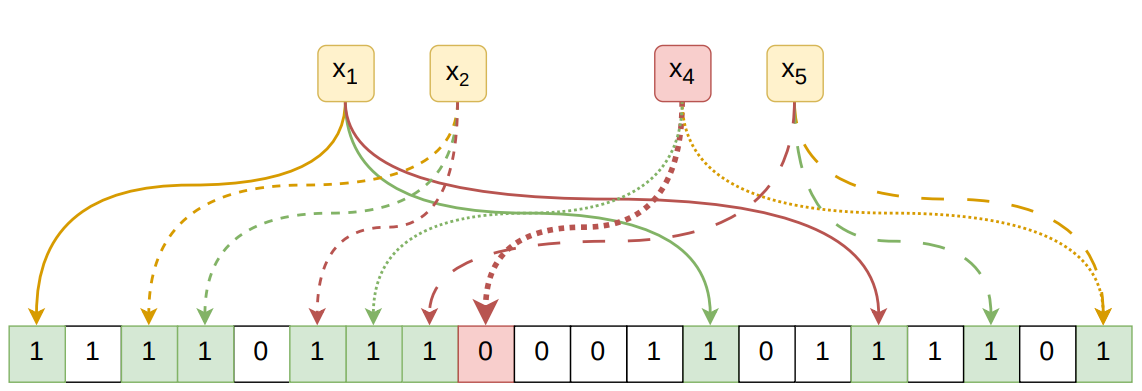
\includegraphics[width=0.5\textwidth]{img/hash/bloom.png}
    \caption{Esempio di query su Bloom Filter}
\end{figure}
\newpage
Una generalizzazione dei Bloom filter sono \textbf{Counting Bloom filter}. In
queste strutture dati si tiene conto anche di quante funzioni di hash mappano in
una certa posizione dato un elemento qualsiasi si verifica la presenza tramite
il counting Bloom filter tramite una threshold $\theta$.

Possiamo costruire questa struttura dati nel seguente modo:
\begin{equation}
    \forall k \in S \text{e} \ \forall h_i \in \mathcal{H}: A[h_i(k)] += 1
\end{equation}
In fase di query, dato $x \in \mathcal{U}$ abbiamo:
\begin{itemize}
    \item Se $\exists h_i \in \mathcal{H}$ tale che $A[h_i(x)] = 0$ o
          $A[h_i(x)] \leq \theta$ allora $x \notin S$
    \item Se $\forall h_i \in \mathcal{H}$ $A[h_i(x)] > 0$ o $A[h_i(x)] > \theta$
          allora "probabilmente" $x \in S$, avendo $\mathcal{P}(FP) \neq 0$
    \item $A[h_i(x)]$ è una sovrastima del numero di elementi $x$ in $S$.
\end{itemize}
\section{Heavy Hitters Problem}
L'\textbf{heavy hitters problem} consiste nell'identificazione dell'elemento più
frequente o anche detto \textbf{heavy hitter}. Questo problema non può essere
risolto utilizzando un \textbf{Bloom Filter} in quanto richiederebbe troppo spazio
di memorizzazione.
\begin{definizione}[\textbf{Stream di dati}]
    Con \textbf{stream di dati} si intende una sequenza di dati passati uno ad
    uno alla struttura dati. Quindi, data una sequenza $S = s_0,s_1, \dots ,s_{n-1}$,
    prima si considera $s_0$, poi $s_1 \ \dots$ fino a $s_{n-1}$ si costruisce
    quindi una struttura dati che può essere interrogata con nuovi valori
    $x \in \mathcal{U}$.
\end{definizione}
Su questa struttura dati è possibile effettuare le seguenti query:
\begin{itemize}
    \item Quante volte appare $x$ nello stream:
          \begin{equation}
              | \{ i \in \{0, 1, \dots, n - 1\}| \ s_i = x \}|
          \end{equation}
    \item Quanti elementi distinti si hanno nello stream:
          \begin{equation}
              |\{s_i | i \in \{0, 1, \dots, n - 1\}\}|
          \end{equation}
\end{itemize}
\subsection{Count-min sketch}
Una struttura dati che ci permette di risolvere questo problema è il
\textbf{Count-min sketch}, la quale richiede poco spazio in memoria ed è
concettualmente simile a un Bloom filter.

Questa struttura dati è definita a partire da:
\begin{itemize}
    \item Insieme universo $\mathcal{U}$.
    \item Uno stream $S$ lungo $n$ costruito da elementi di $\mathcal{U}$.
    \item Due parametri d'errore $\delta$ e $\varepsilon$. Otterremo risposte
          alle query ``sbagliate'' entro un fattore aggiuntivo $\varepsilon$ con
          probabilità almeno $1 - \delta$
    \item $\mathcal{H}, \ |\mathcal{H}| = l = \lceil \ln \frac{1}{\delta} \rceil$,
          famiglia di funzioni hash universale per $\mathcal{U}$ si impone che:
          \begin{equation}
              h_i: \mathcal{U} \to \{0, \dots, m\}, \ \forall h_i \in \mathcal{H},
              \ \text{con} \ m = \left\lceil \frac{e}{\varepsilon} - 1 \right\rceil
          \end{equation}
\end{itemize}
Il \textbf{Count-min sketch} è costituito da una matrice bidimensionale $T$ con
$l$ righe, una per ogni $h_i \in \mathcal{H}$, e $m$ colonne. Si hanno quindi $l$
hash table indipendenti con $m$ entry ciascuna. La matrice $T$ viene inizializzata
con tutti gli elementi a $0$.

Il caricamento di $T$ avviene nel seguente modo:
\begin{itemize}
    \item Si considerano in ordine tutti gli $x_j \in S$, con $j = 0, 1, \dots,
              n - 1$.
    \item Sappiamo che ogni $h_i$ ha di fatto come codominio l'insieme degli indici
          di colonna. Quindi inserire $x_j$ in T vuol dire incrementare di 1
          $T_{h_i} [h_i(x_j)]$, $\forall h_i \in H$
\end{itemize}
Queste operazioni richiedono un tempo per essere eseguite pari a $\mathcal{O}(n)$,
dove $n$ è la lunghezza dello stream.

Su questa struttura dati è possibile eseguire la query per $q \in \mathcal{U}$
nel seguente modo:
\begin{itemize}
    \item Si applica ogni funzione di hash a $q$
    \item Si tiene traccia di ogni $T_{h_i} [h_i(q)]$, $\forall h_i \in \mathcal{H}$
    \item Si restituisce il minimo tra tali valori, che è una stima (una frequenza
          approssimata $\hat{a}_q$) di quante volte occorre $q$ in $S$:
          \begin{equation}
              \hat{a}_q = \min_{h_i \in \mathcal{H}} T_{h_i} [h_i(q)]
          \end{equation}
\end{itemize}
Una query si effettua in tempo $\mathcal{O}(l)$.

È possibile dimostrare che data $a_q$, ovvero la frequenza reale di $q$ in $S$,
si ha che:
\begin{equation}
    a_q \leq \hat{a}_q
\end{equation}
Si dimostra che $a_q \leq \hat{a}_q$ a causa delle collisioni si ottengono
sovrastime ma mai sottostime della frequenza.

Inoltre, è possibile dimostrare:
\begin{equation}
    \hat{a}_q \leq a_q + \varepsilon \cdot n
\end{equation}
con probabilità almeno $1 - \delta$.

Dato che la matrice bidimensionale $T$ è di dimensione $l \times m = \lceil \ln
    \frac{1}{\delta} \rceil \times \lceil \frac{e}{\varepsilon} \rceil$ con
valori che richiedono $\log n$ bit, allora la struttura dati occupa uno spazio
pari a:
\begin{equation}
    \left( \left\lceil \ln \frac{1}{\delta} \right\rceil \cdot \left\lceil
    \frac{e}{\varepsilon} \right\rceil \cdot \log n \right) \ \text{bit}
\end{equation}
\begin{figure}[!ht]
    \centering
    \begin{subfigure}[b]{0.45\textwidth}
        \centering
        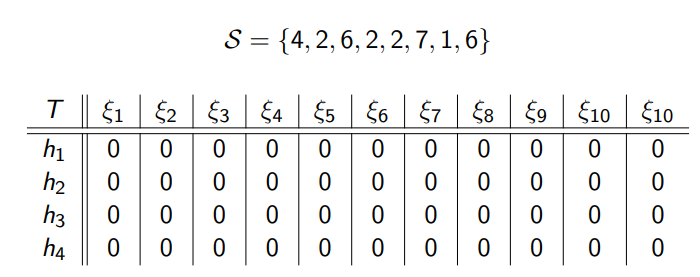
\includegraphics[width=\textwidth]{img/hash/CMS1.png}
        \caption{Inizializzazione}
    \end{subfigure}
    \hfill
    \begin{subfigure}[b]{0.45\textwidth}
        \centering
        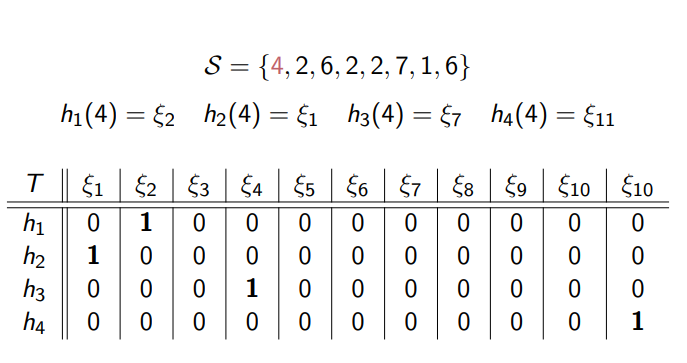
\includegraphics[width=\textwidth]{img/hash/CMS2.png}
        \caption{Inserimento del primo elemento}
    \end{subfigure}
    \hfill
    \begin{subfigure}[b]{0.45\textwidth}
        \centering
        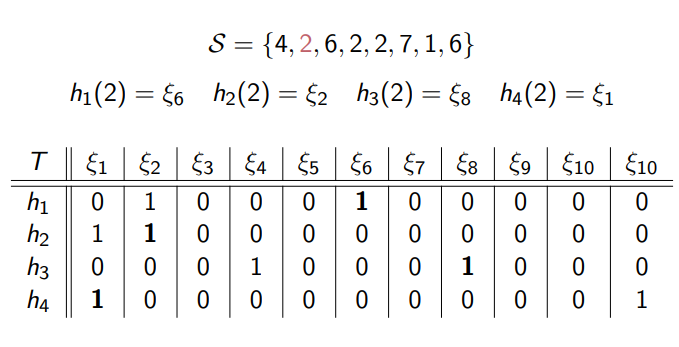
\includegraphics[width=\textwidth]{img/hash/CMS3.png}
        \caption{Inserimento del secondo elemento}
    \end{subfigure}
    \hfill
    \begin{subfigure}[b]{0.45\textwidth}
        \centering
        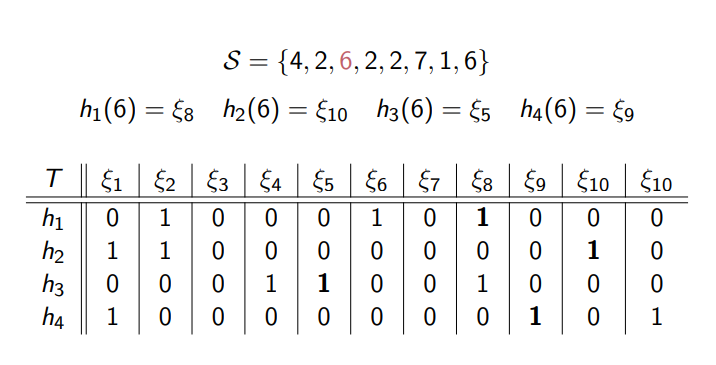
\includegraphics[width=\textwidth]{img/hash/CMS4.png}
        \caption{Inserimento del terzo elemento}
    \end{subfigure}
    \caption{Esempio di riempimento Count-min sketch}
\end{figure}
\chapter{Pattern Matching su Stringhe}
\section{Introduzione}
Il problema del pattern matching consiste cercare un motivo all'interno di un
oggetto più o meno complesso. In questo corso ci si concentrerà sul pattern matching
su stringhe, ovvero cercare all'interno di un testo $T$ le occorrenze di un
pattern $P$.
\begin{definizione}[\textbf{Stringa}]
    Definiamo una \textbf{stringa} $X$ come una giustapposizione di simboli
    appartenenti a un alfabeto $\Sigma$.
    \begin{equation}
        X=x_1x_2\dots x_n \ \ x_i \in \Sigma \ \forall i = 1, \dots, n
    \end{equation}
    In aggiunta, definiremo:
    \begin{itemize}
        \item \textbf{Stringa nulla} $\varepsilon$ è una stringa composta da
              zero simboli.
        \item Simbolo in posizione $i$ si riferisce al simbolo in posizione
              $i$-esima $x_i = X[i]$
        \item \textbf{Sottostringa} da $i$ a $j$ è una porzione di stringa
              compresa tra gli indici $i$ e $j$.
              \begin{equation}
                  X[i, j] = X[i:j] = X[i]X[i+1]\dots X[j - 1]X[j]
              \end{equation}
              Posso esprimerlo attraverso la seguente notazione: $X[i, j] \lor X[i:j]$.
              Possiamo dire che una sottostringa $X[i, j]$ si definisce:
              \begin{itemize}
                  \item \textbf{Propria} se $i \neq 1 \land j \neq |X|$.
                  \item \textbf{Impropria} altrimenti.
              \end{itemize}
        \item \textbf{Prefisso} di lunghezza $j$ è una sottostringa $X[1, j]$.
              Anche in questo caso possiamo distinguere:
              \begin{itemize}
                  \item \textbf{Proprio} se $j \neq |X|$
                  \item \textbf{Improprio} altrimenti.
              \end{itemize}
              Per il prefisso è possibile definire anche il prefisso nullo, ovvero il
              prefisso composto da zero caratteri ($X[1, j]=\varepsilon \ \to \ j = 0$).
        \item \textbf{Suffisso} che inizia in $i$ è la sottostringa $X[i,|X|]$.
              Di questa sottostringa posso calcolare la lunghezza del prefisso come:
              \begin{equation}
                  |X[i,|X|]| = |X| - i + 1
              \end{equation}
              Anche in questo caso possiamo distinguere:
              \begin{itemize}
                  \item \textbf{Proprio} se $i \neq 1$
                  \item \textbf{Improprio} altrimenti.
              \end{itemize}
              È possibile definire il suffisso nullo ovvero quello composto da zero
              caratteri ($X[i,|X|]=\varepsilon \ \to \ i = |X| + 1$).
    \end{itemize}
\end{definizione}
\begin{nota}
    Una \textbf{stringa} di caratteri si differenzia da un \textbf{sequenza}
    degli stessi caratteri dal momento che:
    \begin{itemize}
        \item \textbf{stringa}: è una giustapposizione di caratteri, quindi sono
              tutti concatenati
              \begin{equation}
                  X = \sigma_1\sigma_2\dots\sigma_n
              \end{equation}
        \item \textbf{sequenza}: è un elenco di caratteri separati da un separatore
              \begin{equation}
                  X= \langle\sigma_1,\sigma_2,\dots,\sigma_n\rangle
              \end{equation}
    \end{itemize}
\end{nota}
Quando si parla di string matching possiamo definire due tipi. Dati un pattern
$P$ e un testo $T$ possiamo definire lo string matching:
\begin{enumerate}
    \item \textbf{Esatto}: consiste nel cercare le occorrenze esatte di $P$ in $T$.
    \item \textbf{Approssimato}: consiste nel cercare le occorrenze approssimate
          di $P$ in $T$.
\end{enumerate}
\subsection{String Matching Esatto}
Possiamo definire il problema di \textbf{string matching esatto} formalmente nel
seguente modo:
\begin{itemize}
    \item \textbf{input}: un testo $T$ e un pattern $P$, rispettivamente
          $|T|=n$ e $|P|=m$, definiti su un alfabeto $\Sigma$.
    \item \textbf{output}: tutte le occorrenze esatte $i$ di $T$ ($T[i,i+m-1]=P$).
\end{itemize}
\begin{definizione}[\textbf{Occorrenza esatta}]
    Una posizione $i$ del testo $T$ tale che $T[i, i + m - 1] = P$ è
    un'\textbf{occorrenza esatta} di $P$ in $T$.
\end{definizione}
\begin{definizione}[\textbf{Match}]
    Dati due simboli $s_1, s_2 \in \Sigma$ si ha un \textbf{match} se $s_1 = s_2$.
\end{definizione}
\begin{definizione}[\textbf{Mismatch}]
    Dati due simboli $s_1, s_2 \in \Sigma$ si ha un \textbf{mismatch} se $s_1
        \neq s_2$.
\end{definizione}
Avendo definito il problema in questo modo è possibile definire un semplice
algoritmo che mi permette di calcolare l'output del problema. Questo algoritmo
utilizza una finestra $W$, delle stesse dimensioni del pattern, che scorre sul
testo. L'algoritmo semplice che permette di calcolare le occorrenze esatte è:
\begin{enumerate}
    \item Uso una finestra $W$ lunga $m$ che scorre lungo $T$ da sinistra a
          destra. La posizione iniziale di $W$ è $i = 1$.
    \item Si confronta ogni simbolo di $P$ con il corrispondente simbolo di $T$
          all'interno di $W$ da sinistra verso destra.
          \begin{equation}
              P[j] = T[i + j - 1] \ \forall \ j \ \text{tale che} \ 1 \leq j
              \leq m \ \Rightarrow T[i, i + m - 1] = P
          \end{equation}
    \item $W$ viene spostata di una posizione verso destra e il confronto viene
          ripetuto.
    \item Ultima posizione di $W$ è $i = |T| - |P| + 1 = n - m + 1$
\end{enumerate}
\begin{algorithm}
    \begin{algorithmic}
        \Function{trivial\_exact\_occurrences}{$T, P$}
        \State $n\gets |T|$
        \State $m \gets |P|$
        \State $i\gets 1$
        \While {$i \leq n - m + 1$}
        \State $j \gets 1$
        \While {$P[j] = T[i + j - 1] \ \land \ j \leq m$}
        \State $j \leq j + 1$
        \EndWhile
        \If {$j = m + 1$}
        \State $\text{output } i$
        \EndIf
        \State $i \gets i + 1$
        \EndWhile
        \EndFunction
    \end{algorithmic}
    \caption{Algoritmo banale per String Matching Esatto}
\end{algorithm}
Questo algoritmo richiede un tempo pari a $\mathcal{O}(m \cdot n)$.
\begin{nota}
    Questo algoritmo può essere migliorato spostando la finestra alla posizione
    successiva al primo mismatch oppure si può effettuare un preprocessing del
    pattern e del testo, permettendo di passare da una complessità quadratica ad
    una logaritmica o lineare.
\end{nota}
\subsection{String Matching Approssimato}
Definiremo il problema di \textbf{string matching approssimato} formalmente nel
seguente modo:
\begin{itemize}
    \item \textbf{input}: testo $T$ e un pattern $P$, rispettivamente $|T| = n$ e
          $|P| = m$, definiti entrambi su un alfabeto $\Sigma$, infine, una
          soglia $k$ di errore.
    \item \textbf{output}: tutte le occorrenze approssimate di $P$ in $T$ che
          rispettano la soglia di errore $k$.
\end{itemize}
Introducendo una soglia di errore abbiamo bisogno di definire una metrica per
calcolare l'errore. Per fare ciò si utilizza la \textit{distanza di edit} (ED)
tra due stringhe. Tale distanza è definita come il minimo numero di operazioni di
sostituzione, cancellazione, inserimento di un simbolo che trasformano una
stringa nell'altra.
\begin{nota}
    \begin{equation}
        ED(X_1, X_2) \geq abs(|X_1| - |X_2|)
    \end{equation}
\end{nota}
\begin{definizione}[\textbf{Occorrenza approssimata}]
    Una posizione $i$ del testo $T$, tale che esista almeno una sottostringa
    $S = T[i - L + 1,i]$, con $ED(P, S) \leq k$, che è un'occorrenza approssimata
    di $P$ in $T$.
\end{definizione}
\begin{nota}
    Si può aggiungere:
    \begin{enumerate}
        \item Se $ED(P, S) \leq k$, allora $i$ è occorrenza approssimata.
        \item $ED(P, S) \geq abs(m - L) \ \Rightarrow \ $se $abs(m - L) > k$
              allora $i$ non può essere occorrenza approssimata.
    \end{enumerate}
\end{nota}
Quindi il problema formale dello \textbf{string matching approssimato} verrà
definito come:
\begin{itemize}
    \item \textbf{input}: un testo $T$ e un pattern $P$, rispettivamente $|T| = n$
          e $|P| = m$, definiti entrambi su un alfabeto $\Sigma$, infine, una
          soglia $k$ di errore.
    \item \textbf{output}: tutte le occorrenze approssimate di $P$ in $T$ tale
          che  $ED(P,S)\le k$.
\end{itemize}
Avendo definito il problema in questo modo è possibile definire un semplice
algoritmo che mi permette di calcolare l'output del problema. Questo algoritmo
utilizza una finestra $W$, di dimensione variabile, che scorre sul testo.
\begin{enumerate}
    \item Uso una finestra $W$ di lunghezza variabile $\in [m - k, m + k]$, per
          un totale di $2k+1$ ampiezze da testare, che scorre lungo il testo $T$ da
          sinistra a destra. La posizione iniziale di tale finestra è $i = m - k$ e
          la sua lunghezza iniziale è $m - k$.
    \item Se la distanza di edit tra $P$ e la sottostringa di $T$ compresa in $W$
          è $\leq \ k$, allora $i$ è occorrenza approssimata di $P$ in $T$.
    \item $W$ viene spostata a destra di una posizione.
\end{enumerate}
\begin{algorithm}
    \begin{algorithmic}
        \Function{trivial\_approx\_occurrences}{$T, P, k$}
        \State $n\gets |T|$
        \State $m \gets |P|$
        \State $i\gets m - k$
        \While {$i \leq n$}
        \State $L \gets  m - k$
        \While {$L \leq m + k \ \land \ i - L + 1 \geq 1$}
        \If {$ED(P, T[i - L + 1, i]) \leq k$}
        \State $\text{output } i$
        \EndIf
        \State $L \gets L + 1$
        \EndWhile
        \State $i \gets i + 1$
        \EndWhile
        \EndFunction
    \end{algorithmic}
    \caption{Algoritmo banale per String Matching Approssimato}
\end{algorithm}
Questo algoritmo mi permette di calcolare il matching approssimato in tempo
$\mathcal{O}(n \cdot k \cdot m^2)$, dove $m^2$ è dovuto al calcolo della distanza
di edit tra le due sotto-stringhe.
\section{Ricerca esatta con Automa a Stati Finiti}
Un automa è un modello di calcolo che riconosce un linguaggio, ovvero un insieme
di stringhe che godono di una proprietà. Gli automi a stati finiti riconoscono
un linguaggio regolare.
\begin{definizione} [\textbf{Automa a stati finiti}]
    Un \textbf{Automa a Stati Finiti} è formalmente una quintupla:
    \begin{equation}
        A = (Q, \ \Sigma, \ \delta, \ q_0, \ F)
    \end{equation}
    dove:
    \begin{itemize}
        \item $Q$, insieme \textit{finito} di stati.
        \item $\Sigma$, alfabeto in input.
        \item $\delta: Q \times \Sigma \to Q$, funzione di transizione, dove
              $\delta(q,\sigma)$ rappresenta lo stato di arrivo a partire da $q$
              dopo la lettura di $\sigma$.
        \item $q_0$, stato iniziale.
        \item $F$ (sottoinsieme di $Q$), insieme degli stati accettanti.
    \end{itemize}
\end{definizione}
Gli automi a stati finiti possono essere rappresentati attraverso un diagramma di
stato, ovvero attraverso una struttura a grafo dove i vertici sono gli stati.
Esiste l'arco $(q_1, q_2)$ se almeno un simbolo $\sigma$ è tale per cui $\delta
    (q_1,\sigma) = q_2$. L'arco $(q_1, q_2)$ viene etichettato dalla lista di
simboli che permettono la transizione da $q_1$ a $q_2$. Lo stato iniziale $q_0$
è indicato tramite un arco entrante che non esce da uno stato, mentre gli stati
accettanti sono indicati da un doppio bordo.

È possibile rappresentare la funzione di transizione $\delta$ degli automi
attraverso una matrice $T$ con $|Q|$ righe e $|\Sigma|$ colonne. Nella generica
cella $(q, \sigma)$ sarà contenuto il valore di $\delta(q, \sigma)$, ovvero lo
stato che raggiungo partendo dallo stato $q$ leggendo il simbolo $\sigma$.
\begin{equation}
    T[q,\sigma] = q' \iff \delta(q,\sigma) = q'
\end{equation}
\begin{definizione}[\textbf{Bordo}] \label{def:bordo}
    Il \textbf{bordo} di una stringa $X$ è il più lungo prefisso \textbf{proprio}
    di $X$ che occorre come suffisso di $X$.
\end{definizione}
\begin{esempio}
    Esempi di bordo:
    \begin{itemize}
        \item $X = baaccbbaac$ il suo bordo sarà $B(X) = baac$
        \item $X = aaaccbbaac$ il suo bordo sarà $B(X) = \varepsilon$
        \item $X = abababa$ il suo bordo sarà $B(X) = ababa$
        \item $X = aaaaaaaa$ il suo bordo sarà $B(X) = aaaaaaa$
        \item $X = a$ il suo bordo sarà $B(X) = \varepsilon$
    \end{itemize}
\end{esempio}
\begin{nota}
    Il bordo di una stringa composta da un solo simbolo è sempre vuoto.
\end{nota}
\begin{definizione}[\textbf{Concatenazione}]
    La \textbf{concatenazione} di un simbolo $\sigma$ con la stringa $X$ è la
    stringa $X\sigma$.
\end{definizione}
Possiamo definire ora l'automa a stati finiti per la ricerca esatta di un pattern
$P$ di lunghezza $m$ definito su alfabeto $\Sigma$ come la quintupla $(Q, \Sigma,
    \delta, q_0, F)$ con:
\begin{itemize}
    \item $Q = \{0, 1, \dots, m\}$
    \item $\Sigma$ è l'alfabeto di definizione di $P$.
    \item $\delta: Q \times \Sigma \to Q$ è la funzione di transizione.
    \item $q_0 = 0$ è lo stato iniziale.
    \item $F = \{m\}$ è lo stato accettante.
\end{itemize}
A questo punto, il processo di ricerca esatta attraverso un automa a stati finiti
è composto da:
\begin{enumerate}
    \item \textbf{Preprocessing del pattern}: costruisco l'automa per il pattern
          $P$. Questo punto consiste nel calcolo della funzione di transizione
          $\delta$ in tempo $\Theta(m \cdot |\Sigma|)$.
    \item \textbf{Ricerca nel testo}: uso dell'automa per riconoscere, in un testo
          $T$ definito su alfabeto $\Sigma$, tutte le occorrenze esatte di $P$.
          La scansione del testo $T$ avviene in tempo $\Theta(n)$
\end{enumerate}
\subsection{Funzione di transizione}
La funzione di transizione $\delta$ per un pattern $P$ di lunghezza $m$ definito
su un alfabeto $\Sigma$ è definita per ogni $(j, \sigma) \in Q \times \Sigma$ tale
che $\delta(j, \sigma)$ è lo stato in cui si arriva da $j$ attraverso $\sigma$:
\begin{equation}
    \delta(j, \sigma) = \begin{cases}
        j + 1 & \text{se} \ j < m \ \land \ P[j + 1] = \sigma   \\
        k     & \text{se} \ j = m \ \lor \ P[j + 1] \neq \sigma
    \end{cases}
\end{equation}
dove $k$ è la lunghezza del bordo del prefisso di $P$ di lunghezza $1, j$ a cui
è concatenato $\sigma$, ovvero:
\begin{equation}
    k = |B(P[1, j]\sigma)|, \ \text{con} \ k \leq j
\end{equation}
\begin{itemize}
    \item Dallo stato $0$ si arriva allo stato $0$ per qualsiasi simbolo diverso
          da $P[1]$.
    \item Dallo stato $0$ si arriva allo stato $1$ attraverso il simbolo $P[1]$.
    \item  Dallo stato $j = m$ si arriva sempre a uno stato $k \leq m$, dallo
          stato $m$ si può giungere quindi di nuovo allo stato $m$.
\end{itemize}
\subsubsection{Calcolo della funzione di transizione $\delta$}
L'algoritmo più semplice che permette di calcolare i valori della funzione di
transizione $\delta$ consiste nell'applicare la funzione di transizione $\delta$
per come è definita senza sfruttare i valori che sono già stati computati.
\begin{algorithm}
    \begin{algorithmic}
        \Function{Trivial-build-transition-function}{$P$}
        \State $m \gets |P|$
        \State $\delta \gets empty\_table (m + 1) \times | \Sigma|$
        \For{$j \gets 0 \ \text{to} \ m - 1$}
        \State $\delta(j, P[j + 1]) \gets j + 1$
        \EndFor
        \For{$j \gets 0 \ \text{to} \ m$}
        \For{$\sigma \in \Sigma$}
        \State $\delta(j, \sigma) \gets |B(P[1, j]\sigma)|$
        \EndFor
        \EndFor
        \State \Return $\delta$
        \EndFunction
    \end{algorithmic}
    \caption{Algoritmo banale per il calcolo della funzione di transizione $\delta$}
\end{algorithm}

Questo algoritmo richiede un tempo nel caso peggiore pari a $\mathcal{O}(m^3
    |\Sigma|)$, questo è dovuto al fatto che per calcolare il bordo è necessario
un tempo, nel caso peggiore pari a $\mathcal{O}(m^2)$.

Per migliorare i tempi cambieremo approccio, definiamo $\delta_j$ come la funzione
di transizione di $P[1, j]$, ovvero come una funzione:
\begin{equation}
    \delta_j: \{0, 1, \dots, j\} \times \Sigma \to \{0, 1, \dots, j\}
\end{equation}
per questa funzione possiamo definire due casi particolari:
\begin{itemize}
    \item $\delta_0$ ovvero la funzione di transizione di $P[1, 0]$ che per
          definizione è $\varepsilon$, quindi il valore di tale funzione è sempre
          $0$.
    \item $\delta_m$ ovvero la funzione di transizione di $P[1, m]$ la quale
          corrisponde precisamente alla funzione di transizione del pattern $P$.
\end{itemize}
Possiamo definire il calcolo della funzione di transizione $\delta$ per un pattern
$P$ di lunghezza $m$ utilizzando l'induzione nel seguente modo:
\begin{itemize}
    \item \textbf{Caso base}: calcolo $\delta_0$. Questo risulta banale in quanto
          il valore di $\delta_0$ è sempre $0$.
    \item \textbf{Passo induttivo}: calcolo $\delta_j$ da $\delta_{j - 1}$ in
          questo caso dobbiamo distinguere il caso in cui $j = 1$ e i restanti.
          \begin{itemize}
              \item Nel caso in cui $j = 1$, possiamo definire la funzione di
                    transizione come:
                    \begin{enumerate}
                        \item Prendo il valore $0$ contenuto nella cella della
                              riga $0$ di $\delta_0$ in corrispondenza del
                              simbolo $P[1]$.
                        \item Sostituisco il valore $0$ con il valore $1$ (stato
                              successivo a $0$).
                        \item Aggiungo una nuova riga (corrispondente allo stato
                              $1$)
                        \item Copio la riga che corrisponde allo stato $0$ nella
                              riga che corrisponde allo stato $1$.
                        \item Rinomino $\delta_0$ in $\delta_1$.
                    \end{enumerate}
              \item Mentre nel caso in cui $j \neq 1$ possiamo definire la
                    funzione di transizione come:
                    \begin{enumerate}
                        \item Prendo il valore $k$ contenuto nella cella della
                              riga $j - 1$ di $\delta_{j - 1}$ in corrispondenza
                              del simbolo $P[j]$
                        \item Sostituisco il valore $k$ con il valore $j$ (stato
                              successivo a $j - 1$)
                        \item Aggiungo una nuova riga (corrispondente allo stato
                              $j$)
                        \item Copio la riga che corrisponde allo stato $k$ nella
                              riga che corrisponde allo stato $j$
                        \item Rinomino $\delta_{j - 1}$ in $\delta_j$
                    \end{enumerate}
          \end{itemize}
\end{itemize}
\begin{nota}
    Dimostrazione tramite esempi su slide.
\end{nota}
Con queste informazioni possiamo definire un algoritmo che mi permette di calcolare
la funzione di transizione $\delta$ in tempo $\Theta(m \cdot |\Sigma|)$. Tale
algoritmo sfrutta le informazioni precedentemente calcolate.
\begin{algorithm}[!ht]
    \begin{algorithmic}
        \Function{Build-transition-function}{$P$}
        \State $m \gets |P|$
        \State $\delta \gets empty\_table (m + 1) \times | \Sigma|$
        \For{$\sigma \in \Sigma$}
        \State $\delta(0, \sigma) \gets 0$
        \EndFor
        \For{$j \gets 1 \ \text{to} \ m$}
        \State $k \gets \delta(j - 1, P[j])$
        \State $\delta(j - 1, P[j]) \gets j$
        \For{$\sigma \in \Sigma$}
        \State $\delta(j, \sigma) \gets \delta(k, \sigma)$
        \EndFor
        \EndFor
        \State \Return $\delta$
        \EndFunction
    \end{algorithmic}
    \caption{Algoritmo per il calcolo della funzione di transizione $\delta$}
\end{algorithm}
\subsection{Scansione del testo}
La scansione del testo inizia da uno stato iniziale $j_0 = 0$. Partendo da questo
stato, leggo il simbolo in posizione $i$ del testo ($T[i]$) e mi sposto nello stato
$j_i$ attraverso la funzione di transizione $\delta(j_{i - 1}, T[i])$.
\begin{esempio}
    Consideriamo il testo $T$:
    \begin{table}[!ht]
        \centering
        \begin{tabular}{ccccccc}
            1                       & 2                      & 3
                                    & 4                      & 5
                                    & 6                      & 7 \\ \hline
            \multicolumn{1}{|c|}{c} & \multicolumn{1}{c|}{a} &
            \multicolumn{1}{c|}{b}  & \multicolumn{1}{c|}{a} &
            \multicolumn{1}{c|}{c}  & \multicolumn{1}{c|}{a} &
            \multicolumn{1}{c|}{b}                               \\ \hline
        \end{tabular}
    \end{table}

    e il pattern $P$:
    \begin{table}[!ht]
        \centering
        \begin{tabular}{ccccccc}
            1                       & 2                      & 3
                                    & 4                          \\ \hline
            \multicolumn{1}{|c|}{a} & \multicolumn{1}{c|}{c} &
            \multicolumn{1}{c|}{a}  & \multicolumn{1}{c|}{c}     \\ \hline
        \end{tabular}
    \end{table}

    Su cui è stata definita la seguente funzione di transizione $\delta$:
    \begin{table}[!ht]
        \centering
        \begin{tabular}{|>{\columncolor[HTML]{EFEFEF}}c |c|c|c|} \hline
            $\delta$                           &
            \cellcolor[HTML]{EFEFEF}\textbf{a} &
            \cellcolor[HTML]{EFEFEF}\textbf{b} &
            \cellcolor[HTML]{EFEFEF}\textbf{c}             \\ \hline
            \textbf{0}                         & 1 & 0 & 0 \\ \hline
            \textbf{1}                         & 1 & 0 & 2 \\ \hline
            \textbf{2}                         & 3 & 0 & 0 \\ \hline
            \textbf{3}                         & 1 & 0 & 4 \\ \hline
            \textbf{4}                         & 3 & 0 & 0 \\ \hline
        \end{tabular}
    \end{table}

    La scansione del testo $T$ cercando le occorrenze esatte del pattern $P$ mi
    permette di ottenere il risultato riportato in figura \ref{fig:scansione}
    \begin{figure}[!ht]
        \centering
        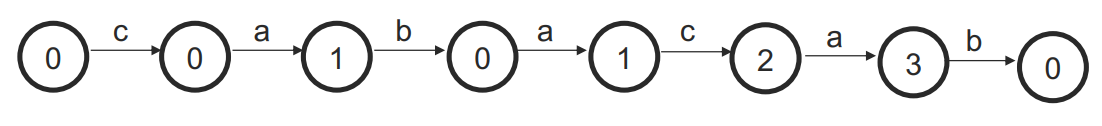
\includegraphics[width=0.5\textwidth]{img/pattern/ScansioneTesto.png}
        \caption{Risultato della scansione del testo}
        \label{fig:scansione}
    \end{figure}
\end{esempio}
A questo punto è necessario identificare un'occorrenza esatta del pattern $P$
nel testo $T$. Per risolvere questo, partiamo dalla successione di stati che
abbiamo definito per la scansione del testo. Essa corrisponde a una successione
di posizioni su $P$, o in altre parole, a una successione di lunghezze di
prefissi del pattern $P$.
\begin{teorema}
    $j_i$, con $0 \leq i \leq n$, è la lunghezza del \textbf{più lungo} prefisso
    di $P$ uguale a una sottostringa di $T$ che finisce in posizione $i$.
\end{teorema}
\begin{dimostrazione}
    È possibile dimostrare il teorema precedente con una dimostrazione per
    induzione:
    \begin{enumerate}
        \item \textbf{Caso base}: per lo stato $j_0 = 0$ il teorema è banalmente
              dimostrabile, in quanto il prefisso di lunghezza $0$ è il prefisso
              nullo che è sottostringa di $T$.
        \item \textbf{Passo induttivo}: se $j_{i - 1}$ è la lunghezza del più
              lungo prefisso di $P$ uguale alla sottostringa di $T$ che finisce
              in posizione $i - 1$, allora $j_i$ è la lunghezza del più lungo
              prefisso di $P$ uguale alla sottostringa di $T$ che finisce in
              posizione $i$.

              Per dimostrare il passo induttivo ci basiamo sulla seguente ipotesi:
              $j_{i - 1}$ è la lunghezza del più lungo prefisso di $P$ uguale a
              una sottostringa di $T$ che finisce in posizione $i - 1$.
              \begin{itemize}
                  \item \textbf{Caso 1}: $j_{i - 1} < m$ e $P[j_{i - 1} + 1] =
                            T[i]$ questo implica $j_i = \delta(j_{i - 1}, T[i])
                            = j_{i - 1} + 1$
                        \begin{itemize}
                            \item $j_{i - 1} \neq 0$: la tesi è confermata.
                            \item $j_{i - 1} = 0$ vuol dire che il carattere
                                  corrisponde con il carattere iniziale del pattern.
                        \end{itemize}
                  \item \textbf{Caso 2}: $j_{i - 1} = m$ oppure $P[j_{i - 1} + 1]
                            \neq T[i]$ questo implica $j_i = \delta(j_{i - 1},
                            T[i]) = k$ dove $k$ è la lunghezza del bordo di
                        $P[1, j_{i - 1}]T[i]$.
                        \begin{itemize}
                            \item $0 < j_{i - 1} < m$: in questo caso il valore
                                  di $k$ mi rappresenta una parte del testo per
                                  cui ho già verificato un'occorrenza esatta,
                                  questo mi viene garantito dalla definizione di
                                  bordo.
                            \item $j_{i - 1} = 0$ vuol dire che sono rimasto
                                  nello stato 0.
                            \item $j_{i - 1} = m$ ho trovato un'occorrenza esatta
                                  del pattern, inoltre per evitare di perdere delle
                                  occorrenze mi sposto in base alla lunghezza del
                                  bordo del pattern concatenato con il carattere
                                  successivo.
                        \end{itemize}
              \end{itemize}
    \end{enumerate}
\end{dimostrazione}
Questo teorema mi fornisce la garanzia che non sto perdendo delle occorrenze.
Inoltre, posso trovare la posizione di inizio dell'occorrenza esatta come $i - j
    + 1$. Nel caso in cui $j_i = m$ ho identificato un'occorrenza esatta del
pattern $P$.

Possiamo riassumere la scansione del testo come:
\begin{enumerate}
    \item Si parte dallo stato iniziale $0$ e si effettua una scansione di $T$
          dal primo all'ultimo simbolo.
    \item Per ogni posizione $i$ di $T$ si effettua la transizione dallo stato
          corrente $j_c$ al nuovo stato $j_f = \delta(j_c, T[i])$.
    \item Ogni volta che lo stato $j_f$ è lo stato accettante ($m$), viene prodotta
          in output l'occorrenza $i - m + 1$.
\end{enumerate}
\begin{algorithm}
    \begin{algorithmic}
        \Function{ASF\_exact\_occurrences}{$\delta, T, m$}
        \State $n \gets |T|$
        \State $j \gets 0$
        \For{$i \gets 1 \ \text{to} \ n$}
        \State $j \gets \delta(j, T[i])$
        \If{$j = m$}
        \State $\text{\textbf{Output}} \ i - m + 1$
        \EndIf
        \EndFor
        \EndFunction
    \end{algorithmic}
    \caption{Algoritmo per la ricerca esatta con Automa a Stati Finiti}
\end{algorithm}
Questo algoritmo viene eseguito in tempo $\Theta(n)$.
\begin{esempio}
    Consideriamo il testo $T$:
    \begin{table}[!ht]
        \centering
        \begin{tabular}{ccccccccccccc}
            1                       & 2                      & 3
                                    & 4                      & 5
                                    & 6                      & 7
                                    & 8                      & 9
                                    & 10                     & 11
                                    & 12                     & 13 \\ \hline
            \multicolumn{1}{|c|}{c} & \multicolumn{1}{c|}{a} &
            \multicolumn{1}{c|}{b}  & \multicolumn{1}{c|}{a} &
            \multicolumn{1}{c|}{c}  & \multicolumn{1}{c|}{a} &
            \multicolumn{1}{c|}{c}  & \multicolumn{1}{c|}{b} &
            \multicolumn{1}{c|}{a}  & \multicolumn{1}{c|}{c} &
            \multicolumn{1}{c|}{a}  & \multicolumn{1}{c|}{b} &
            \multicolumn{1}{c|}{a}                                \\ \hline
        \end{tabular}
    \end{table}

    e il pattern $P$:
    \begin{table}[!ht]
        \centering
        \begin{tabular}{ccccccc}
            1                       & 2                      & 3
                                    & 4                      & 5
                                    & 6                      & 7 \\ \hline
            \multicolumn{1}{|c|}{a} & \multicolumn{1}{c|}{c} &
            \multicolumn{1}{c|}{a}  & \multicolumn{1}{c|}{c} &
            \multicolumn{1}{c|}{b}  & \multicolumn{1}{c|}{a} &
            \multicolumn{1}{c|}{c}                               \\ \hline
        \end{tabular}
    \end{table}

    Su cui è stata definita la seguente funzione di transizione $\delta$:
    \begin{table}[!ht]
        \centering
        \begin{tabular}{|>{\columncolor[HTML]{EFEFEF}}c |c|c|c|} \hline
            $\delta$                           &
            \cellcolor[HTML]{EFEFEF}\textbf{a} &
            \cellcolor[HTML]{EFEFEF}\textbf{b} &
            \cellcolor[HTML]{EFEFEF}\textbf{c}             \\ \hline
            \textbf{0}                         & 1 & 0 & 0 \\ \hline
            \textbf{1}                         & 1 & 0 & 2 \\ \hline
            \textbf{2}                         & 3 & 0 & 0 \\ \hline
            \textbf{3}                         & 1 & 0 & 4 \\ \hline
            \textbf{4}                         & 3 & 5 & 0 \\ \hline
            \textbf{5}                         & 6 & 0 & 0 \\ \hline
            \textbf{6}                         & 1 & 0 & 7 \\ \hline
            \textbf{7}                         & 3 & 0 & 0 \\ \hline
        \end{tabular}
    \end{table}

    Otteniamo la seguente esecuzione dell'algoritmo:
    \begin{figure}[!ht]
        \centering
        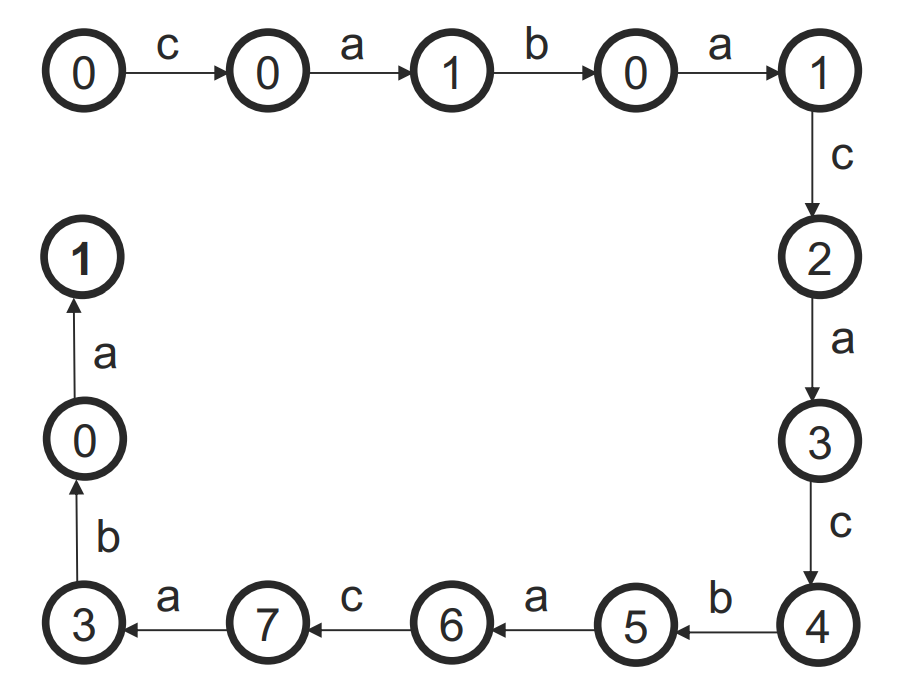
\includegraphics[width=0.3\textwidth]{img/pattern/ASF.png}
        \caption{Esecuzione dell'algoritmo per la ricerca esatta con Automa a
            Stati Finiti}
        \label{fig:enter-label}
    \end{figure}
\end{esempio}
\newpage
\section{Algoritmo di Knuth-Morris-Pratt}
Questo algoritmo per la ricerca esatta è basato su un'analisi del pattern. Si
hanno due fasi:
\begin{enumerate}
    \item \textbf{Preprocessing del pattern}: questa fase consiste nel calcolo
          della \textbf{prefix function} $\phi$, che è una funzione che associa
          ad ogni posizione del pattern la lunghezza del più lungo prefisso del
          pattern che è anche un suffisso del pattern. Questa funzione è calcolata
          in tempo lineare rispetto alla lunghezza del pattern $\mathcal{O}(m)$.
    \item \textbf{Scansione del testo}: questa fase consiste nel confrontare il
          pattern con il testo cercando di identificare le occorrenze esatte di
          esso. Questa fase è eseguita in tempo lineare rispetto alla lunghezza
          del testo $\mathcal{O}(n)$.
\end{enumerate}
La \textbf{prefix function} o funzione di fallimento $\phi$ è definita come segue:
\begin{equation}
    \phi: \{0, 1, \dots m\} \to \{-1, 0, \dots m\}
\end{equation}
\begin{nota}
    La funzione di fallimento $\phi$ è definita su un insieme di indici che va
    da $0$ a $m - 1$ in quanto è definita come il bordo del pattern. Per definizione
    di bordo (\ref{def:bordo}) è un prefisso proprio, quindi non può assumere il
    valore $m$.
\end{nota}
Essa è definita come segue:
\begin{equation}
    \phi(j) = \begin{cases}
        |B(P[1, j])| & \text{se } 1 \leq j \leq m \\
        -1           & \text{se } j = 0
    \end{cases}
\end{equation}
\begin{esempio}
    Calcoliamo $\phi$ sul pattern $P=abcabaabcabab$ con $m=13$.
    \begin{table}[!ht]
        \centering
        \begin{tabular}{|>{\columncolor[HTML]{EFEFEF}}c|c|c|c|c|c|c|c|c|c|c|c|c|c|c|}\hline
            \cellcolor[HTML]{EFEFEF}\textbf{j}  &
            \cellcolor[HTML]{EFEFEF}\textbf{0}  &
            \cellcolor[HTML]{EFEFEF}\textbf{1}  &
            \cellcolor[HTML]{EFEFEF}\textbf{2}  &
            \cellcolor[HTML]{EFEFEF}\textbf{3}  &
            \cellcolor[HTML]{EFEFEF}\textbf{4}  &
            \cellcolor[HTML]{EFEFEF}\textbf{5}  &
            \cellcolor[HTML]{EFEFEF}\textbf{6}  &
            \cellcolor[HTML]{EFEFEF}\textbf{7}  &
            \cellcolor[HTML]{EFEFEF}\textbf{8}  &
            \cellcolor[HTML]{EFEFEF}\textbf{9}  &
            \cellcolor[HTML]{EFEFEF}\textbf{10} &
            \cellcolor[HTML]{EFEFEF}\textbf{11} &
            \cellcolor[HTML]{EFEFEF}\textbf{12} &
            \cellcolor[HTML]{EFEFEF}\textbf{13}                                  \\	\hline
            $\phi$                              & -1 & 0 & 0 & 0 & 1 & 2 & 1 & 1
                                                & 2  & 3 & 4 & 5 & 6 & 2         \\\hline
        \end{tabular}
    \end{table}
\end{esempio}
\newpage
Questo algoritmo è un'evoluzione dell'algoritmo banale per la ricerca delle
occorrenze di un pattern in un testo. In particolare, l'algoritmo KMP consiste in:
\begin{enumerate}
    \item Viene usata una finestra $W$ di lunghezza $m$ che scorre sul testo $T$
          da sinistra a destra con posizione iniziale $i = 1$.
    \item Si confrontano i simboli di $P$ con i corrispondenti simboli di $T$
          all'interno della finestra $W$ andando da sinistra a destra e partendo
          dal primo simbolo di $P$.
    \item Non appena si incontra un \textit{mismatch} oppure ogni simbolo di $P$
          ha un match con il corrispondente simbolo in $W$ (i è occorrenza esatta),
          $W$ viene spostata a destra nella posizione:
          \begin{equation}
              p = i + j - \phi(j - 1) - 1
          \end{equation}
          dove $j$ è l'indice del simbolo di $P$ che ha causato il mismatch,
          mentre $i$ è la posizione iniziale di $W$.
    \item L'ultima posizione di $W$ è $n - m + 1$.
\end{enumerate}
Riassumendo:
\begin{itemize}
    \item $W$ viene spostata dalla posizione $i$ alla posizione $p$, dove:
          \begin{equation}
              p = i + j - \phi(j - 1) - 1
          \end{equation}
          con $j$ indice del simbolo di $P$ che ha causato il mismatch per $W$
          in posizione $i$.
    \item Il confronto riparte dal simbolo di $P$ in posizione $j = \phi(j - 1)
              + 1$ e dal simbolo di $T$ in posizione $i + j - 1$.
\end{itemize}
Nel caso in cui $j = 1$, allora $p = i + 1$ e il confronto riparte dal primo
simbolo di $P$ e dal simbolo di $T$ in posizione $i + 1$.
\begin{nota}
    Chiaramente il confronto riparte dalle posizioni $i + 1$ su $T$ e $1$ su P,
    ma dire che riparte dalla posizione $i$ su $T$ e dalla posizione $0$ su $P$
    implicitamente fa riferimento ad un confronto iniziale fittizio tra $T[i]$ e
    $P[0]$ (simbolo inesistente) che di default viene considerato un match.
\end{nota}
Nel caso in cui $j = m + 1$, allora $p = i + m - \phi(m)$ e il confronto
riparte dalla posizione $\phi(m) + 1$ di $P$ e dal simbolo di $T$ in posizione
$i + m$.
\begin{table}[!ht]
    \centering
    \begin{tabular}{|l|l|l|}
        \hline
                           & Automa a stati finiti     & KMP              \\ \hline
        Preprocessing di P & $\mathcal{O}(m |\Sigma|)$ & $\mathcal{O}(m)$ \\ \hline
        Scansione di T     & $\mathcal{O}(n)$          & $\mathcal{O}(n)$ \\ \hline
        Spazio             & $\mathcal{O}(m |\Sigma|)$ & $\mathcal{O}(m)$ \\ \hline
    \end{tabular}
\end{table}
Le differenze tra l'algoritmo basato sull'automa a stati finiti e KMP sono:
\begin{itemize}
    \item Automa:
          \begin{itemize}
              \item Efficiente per pattern piccoli, perché la memoria è contenuta
                    quindi le costanti all'interno del calcolo del tempo sono
                    migliori.
              \item Richiede più tempo e memoria per pattern grandi, perché
                    sprechiamo tempo nel calcolo del $\delta$.
              \item Ricerca di P in testi diversi utilizzando lo stesso automa.
          \end{itemize}
          KMP:
          \begin{itemize}
              \item Efficiente per pattern grandi.
              \item Richiede più tempo per pattern piccoli.
          \end{itemize}
\end{itemize}
\section{Algoritmo di Baeza-Yates e Gonnet}
La ricerca esatta effettuata attraverso questo algoritmo effettua un confronto
tra i simboli del pattern e del testo in maniera non esplicita, ovvero non
confronta carattere per carattere. In questo algoritmo vengono effettuate in
parallelo operazioni bit a bit su word di bit, viene anche chiamato
\textit{algoritmo bit parallel}.

Questo algoritmo segue il paradigma \textbf{shift-and} ovvero compie fondamentalmente
due sole operazioni:
\begin{itemize}
    \item \textbf{Shift} dei bit.
    \item \textbf{AND} logico tra i bit.
\end{itemize}
Come gli algoritmi visti fin ora, anche in questo caso possiamo descrivere il suo
funzionamento attraverso due fasi:
\begin{itemize}
    \item \textbf{Preprocessing del pattern} $P$ nel quale vengono calcolate
          $|\Sigma|$ \textbf{words} ognuna di $m$ bit. Questa operazione viene
          eseguita in tempo $\Theta(m + |\Sigma|)$.
    \item \textbf{Scansione del testo} $T$ per cercare le occorrenze esatte del
          pattern $P$. Questa operazione viene eseguita in tempo $\Theta(n)$.
\end{itemize}
\subsection{Word e Operatori}
\begin{definizione}[\textbf{Word di bit}]
    Una \textbf{word di bit} è un gruppo di bit che viene trattato come un'unità
    la cui dimensione può variare e che rappresenta un valore di un certo tipo,
    come ad esempio un numero o un carattere. In una word, il bit più a destra è
    quello meno significativo, mentre quello più a sinistra è quello più significativo.
\end{definizione}
Sulle word si possono eseguire delle operazioni \textit{bit a bit}, ovvero si
esegue un'operazione tra i bit corrispondenti di due o più words di bit della
stessa lunghezza. Il valore restituito da queste operazioni è una nuova word in
cui ogni bit è il risultato dell'operazione tra i bit corrispondenti nelle word
in input. Tra queste operazioni abbiamo:
\begin{itemize}
    \item \textbf{Congiunzione logica} $\to$ AND. Questa operazione è implementata
          come:
          \begin{equation}
              w = w_1 \ \text{AND} \ w_2
          \end{equation}
          restituisce una word $w$ tale che:
          \begin{equation}
              w[j] = \begin{cases}
                  1 & \text{se } w_1[j] = 1 \ \text{AND} \ w_2[j] = 1 \\
                  0 & \text{altrimenti}
              \end{cases}
          \end{equation}
    \item \textbf{Disgiunzione logica} (inclusiva) $\to$ OR. Questa operazione è
          implementata come:
          \begin{equation}
              w = w_1 \ \text{OR} \ w_2
          \end{equation}
          restituisce una word $w$ tale che:
          \begin{equation}
              w[j] = \begin{cases}
                  1 & \text{se } w_1[j] = 1 \ \text{OR} \ w_2[j] = 1 \\
                  0 & \text{altrimenti}
              \end{cases}
          \end{equation}
    \item \textbf{Shift dei bit} di una posizione a destra con bit più significativo
          a $0$ $\to$ RSHIFT. Questa operazione è implementata come:
          \begin{equation}
              w = \text{RSHIFT}(w_1)
          \end{equation}
          restituisce una word $w$ tale che:
          \begin{itemize}
              \item $w[j] = w_1[j - 1]$ se $j \geq 2$.
              \item $w[1] = 0$ altrimenti.
          \end{itemize}
    \item \textbf{Shift dei bit} di una posizione a destra con bit più significativo
          a $1$ $\to$ RSHIFT1. Questa operazione viene implementata come un RSHIFT
          seguito da un OR con una maschera in cui nella prima posizione è presente
          1 e nelle altre 0.
\end{itemize}
\subsection{Preprocessing del pattern} \label{subsec:preprocessing}
Dato un pattern $P$ di lunghezza $m$ e un carattere $\sigma$ appartenete
all'alfabeto $\Sigma$, $B_{\sigma}$ è una word di $m$ bit definita come:
\begin{equation}
    B_{\sigma}[j] = 1 \iff P[j] = \sigma
\end{equation}
Viene creata una word per ogni simbolo dell'alfabeto $\Sigma$ e viene memorizzata
in una tabella $B$. Con questa rappresentazione posso effettuare le query del tipo:
\begin{center}
    Il simbolo in posizione $j$ di $P$ è uguale a un certo simbolo $\sigma$
\end{center}
\begin{esempio}
    Calcoliamo la tabella $B$ per un pattern $P=abcaba$ su un alfabeto $\Sigma =
        \{a, b, c, d\}$.
    \begin{table}[!ht]
        \centering
        \begin{tabular}{|c|c|c|c|c|c|c|}
            \hline
            P     & a & b & c & a & b & a \\ \hline
            $B_a$ & 1 & 0 & 0 & 1 & 0 & 1 \\ \hline
            $B_b$ & 0 & 1 & 0 & 0 & 1 & 0 \\ \hline
            $B_c$ & 0 & 0 & 1 & 0 & 0 & 0 \\ \hline
            $B_d$ & 0 & 0 & 0 & 0 & 0 & 0 \\ \hline
        \end{tabular}
    \end{table}
\end{esempio}
Vediamo ora come calcolare la tabella $B$:
\begin{enumerate}
    \item Tutte le word $B_{\sigma}$ vengono inizializzate a $m$ bit a $0$.
    \item Viene creata una maschera $M$ di $m$ bit tutti uguali a $0$ tranne il
          più significativo che è uguale a $1$.
    \item Si esegue una scansione di $P$ da sinistra a destra, e per ogni posizione
          $j$ vengono eseguite le due operazioni bit a bit:
          \begin{itemize}
              \item $B_{P[j]} = M \ \textbf{OR} \ B_{P[j]}$
              \item $M = \textbf{RSHIFT} (M)$
          \end{itemize}
\end{enumerate}
L'algoritmo per calcolare la tabella richiede un tempo pari a $\Theta(|\Sigma| +
    m)$ ed è il seguente:
\begin{algorithm}
    \begin{algorithmic}
        \Function{Compute-table-B}{$P$}
        \State $m \gets |P|$
        \State $B \gets \text{empty table of} \ |\Sigma| \ \text{words} \ B_{\sigma}$
        \For{$\sigma \in \Sigma$}
        \State $B_{\sigma} \gets 00\dots0$
        \EndFor
        \State $M \gets 10\dots0$
        \For{$\sigma \in \Sigma$}
        \State $\sigma \gets P[j]$
        \State $B_{\sigma} \gets M \ \text{OR} \ B_{\sigma}$
        \State $M = \textbf{RSHIFT} (M)$
        \EndFor
        \State \textbf{return} $B$
        \EndFunction
    \end{algorithmic}
    \caption{Algoritmo per il calcolo della tabella $B$}
\end{algorithm}
\subsection{Scansione del testo}
La procedura per la scansione del testo è rappresentata come:
\begin{enumerate}
    \item Il testo $T$ viene scandito dalla prima all'ultima posizione.
    \item Per ogni posizione $i$ del testo $T$ viene calcolata una word $D_i$ di
          $m$ bit.
    \item Ogni volta che in $D_i$ il bit meno significativo è uguale a $1$, allora
          $i - m + 1$ è occorrenza esatta di $P$ in $T$.
\end{enumerate}
Dobbiamo ora definire cosa si intende con la word $D_i$. Prima di fare ciò dobbiamo
definire $P[1,j] = suff(T[1,i])$ ovvero $P[1,j]$ è uguale a un suffisso di $T[1,i]$.
\begin{definizione}[\textbf{Word $D_i$}] \label{def:word}
    Dati un pattern $P$ lungo $m$ e un testo $T$ lungo $n$, $D_i$ ($0 \leq i \leq
        n$) è una word di $m$ bit tale che:
    \begin{equation}
        D_i[j] = 1 \iff P[1,j] = suff(T[1,i])
    \end{equation}
    Inoltre, sappiamo per definizione che:
    \begin{itemize}
        \item $D_0 = 00\dots0$ dato che $P[1, j] \neq suff(T[1, 0]) \ \forall j$
        \item $D_i[m] = 1$ se e solo se $P[1, m] = suff(T[1, i]) = T[i - m + 1,
                          i]$ ovvero si ha un'occorrenza esatta di $P$ in $T$
              nella posizione $i - m + 1$.
    \end{itemize}
\end{definizione}
\begin{nota}
    Nota che da $D_i$ possiamo anche ottenere la lunghezza del bordo del pattern.
    In generale, data una word $D_i$, la lunghezza del bordo del pattern $P$ è
    uguale a $j$ se e solo se $D_i[m] = 1$ e $j$ è la più grande posizione $< m$
    tale che $D_i[j] = 1$.

    Con posizione più grande si intende quella più a destra diversa da $m$.
\end{nota}
\begin{esempio}
    Data la word riportata nella tabella \ref{tab:word}, possiamo calcolare il
    bordo del pattern in quanto l'ultimo bit è uguale a $1$.
    \begin{table}[!ht]
        \centering
        \begin{tabular}{|c|c|c|c|c|c|c|c|c|c|c|c|c|c|c|c|c|}
            \hline
            $D_i$ & 0 & 1 & 1 & 0 & 0 & 0 & 1 & 1 & 0 & 0  & 1  & 0  & 0  & 0  & 0  & 1  \\ \hline
                  & 1 & 2 & 3 & 4 & 5 & 6 & 7 & 8 & 9 & 10 & 11 & 12 & 13 & 14 & 15 & 16 \\ \hline
        \end{tabular}
        \caption{Word $D_i$}
        \label{tab:word}
    \end{table}

    Dato che il bit con valore uguale a $1$ più a destra, diverso da $m$, è in
    posizione $11$, allora la lunghezza del bordo è:
    \begin{equation}
        |B(P)| = 11
    \end{equation}
\end{esempio}
Ovviamente calcolare $D_i$ è sempre troppo costoso, infatti, $D_i$ viene sempre
ottenuto a partire da $D_{i - 1}$, portando a modificare l'algoritmo di scansione
del testo nel seguente modo:
\begin{itemize}
    \item Inizia dalla word $D_0 = 00\dots0$
    \item Per ogni $i$ da $1$ a $n$ calcola la word $D_i$ a partire dalla word
          $D_{i - 1}$.
    \item Ogni volta che $D_i$ ha il bit meno significativo uguale a $1$, viene
          prodotta in output l'occorrenza $i - m + 1$.
\end{itemize}
Vediamo ora come si calcola il valore di $D_i$ a partire da $D_{i - 1}$:
\begin{itemize}
    \item Se $j =  1$ allora posso calcolarla come:
          \begin{equation}
              D_i[1] = 1 \ \textbf{AND} \ B_{T[i]}[1]
          \end{equation}
          Perché $D_i[1] = 1 \iff P[1,1] = suff(T[1,i]) \iff P[1] = T[i] \iff
              B_{T[i]}[1]$. Si aggiunge $1$ per semplificare le operazioni bit
          a bit.
    \item Se $j > 1$ allora posso calcolarla come:
          \begin{equation}
              D_i[j] = D_{i - 1}[j - 1] \ \textbf{AND} \ B_{T[i]}[j]
          \end{equation}
          Perché $D_i[j] = 1 \iff P[1,j] = suff(T[1,i]) \iff P[1,j - 1] =
              suff(T[1,i - 1]) \ \textbf{AND} \ P[j] = T[i] \iff D_{i - 1}[j - 1]
              \ \textbf{AND} \ B_{T[i]}[j]$.
\end{itemize}
In questo modo stiamo ancora aggiornando un bit alla volta, ma sfruttando le
operazioni bit a bit si possono aggiornare tutti in tempo \textbf{costante} nel
seguente modo:
\begin{equation}
    D_i = \textbf{RSHIFT1}(D_{i - 1}) \ \textbf{AND} \ B_{T[i]}
\end{equation}
Vediamo ora come implementare l'algoritmo che effettua la scansione del testo in
tempo $\Theta(n)$.
\begin{algorithm}
    \begin{algorithmic}
        \Function{BYG}{$B, T$}
        \State $n \gets |T|$
        \State $D \gets 00\dots0$
        \State $M \gets 00\dots01$
        \For{$i \gets 1 \ \text{to} \ n$}
        \State $\sigma \gets T[i]$
        \State $D \gets \textbf{RSHIFT1}(D_{i - 1}) \ \textbf{AND} \ B_{T[i]}$
        \If{$(D \ \textbf{AND} M) = M$}
        \State \text{output} $i - m + 1$
        \EndIf
        \EndFor
        \EndFunction
    \end{algorithmic}
    \caption{Algoritmo per la scansione del testo}
\end{algorithm}
\newpage
\begin{esempio}
    Siano un testo $T = babcabaadc$ e un pattern $P = abcaba$ tale che $|T| = 10$
    e $|P|=6$. Entrambe le stringhe costruite su un alfabeto $\Sigma = \{a, b, c,
        d\}$, allora costruiamo la tabella $B_\sigma$:
    \begin{table}[!ht]
        \centering
        \begin{tabular}{|c|c|c|c|c|c|c|}
            \hline
            P     & $a$ & $b$ & $c$ & $a$ & $b$ & $a$ \\ \hline
            $B_a$ & $1$ & $0$ & $0$ & $1$ & $0$ & $1$ \\ \hline
            $B_b$ & $0$ & $1$ & $0$ & $0$ & $1$ & $0$ \\ \hline
            $B_c$ & $0$ & $0$ & $1$ & $0$ & $0$ & $0$ \\ \hline
            $B_d$ & $0$ & $0$ & $0$ & $0$ & $0$ & $0$ \\ \hline
        \end{tabular}
    \end{table}
    I singoli passi sono i seguenti:
    \begin{itemize}
        \item Quindi partiremo da $D_0 = 000000$, leggo il primo simbolo del
              testo $T[1] = b$ e poi calcolo:
              \begin{equation}
                  D_1=RSHIFT1(D_{0}) \text{ AND } B_b = 100000 \text{ AND }
                  010010 = 000000
              \end{equation}
        \item Leggo il secondo simbolo del testo $T[2] = a$ e poi calcolo $D_2$:
              \begin{equation}
                  D_2 = 100000 \text{ AND } 100101 = 100000
              \end{equation}
        \item Leggo il secondo simbolo del testo $T[3] = b$ e poi calcolo $D_3$:
              \begin{equation}
                  D_3 = 110000 \text{ AND } 010010 = 010000
              \end{equation}
        \item Leggo il secondo simbolo del testo $T[4] = c$ e poi calcolo $D_4$:
              \begin{equation}
                  D_4 = 101100 \text{ AND } 001000 = 001000
              \end{equation}
        \item Leggo il secondo simbolo del testo $T[5] = a$ e poi calcolo $D_5$:
              \begin{equation}
                  D_5 = 100100 \text{ AND } 100101 = 100100
              \end{equation}
        \item $\dots$
        \item Leggo il secondo simbolo del testo $T[7] = a$ e poi calcolo $D_7$
              \begin{equation}
                  D_6 = 101001 \text{ AND } 100101 = 100001
              \end{equation}
        \item Ho il bit LSB di $D_6$ uguale a $1$, quindi ho trovato un match che
              corrisponde a $i - m + 1 = 7 - 6 + 1 = 2$. Poi continuo fino a
              quando non termino $T$.
    \end{itemize}
\end{esempio}
\section{Algoritmo di Wu e Manber}
L'algoritmo risolvere problemi di \textbf{string matching approssimati} e il
funzionamento è simile all'algoritmo \textbf{BYG}.
Riprendiamo la definizione di ricerca approssimata di un pattern $P$ in un testo
$T$:
\begin{definizione}[\textbf{Occorrenza approssimata}]
    Una posizione $i$ del testo $T$ tale che esista una sottostringa $S = T[i -
                L + 1]$ tale che $ED(P, S) \leq k$ è detta \textbf{occorrenza
        approssimata} di $P$ in $T$.
\end{definizione}
Come gli algoritmi visti fino a questo momento, anche quello di Wu e Manber è
strutturato in due fasi:
\begin{enumerate}
    \item \textbf{Preprocessing del pattern} $P$: in questa fase vengono calcolate
          $|\Sigma|$ \textbf{words} ognuna di $m$ bit. Questa operazione viene
          eseguita in tempo $\Theta(|\Sigma| + m)$. (\textit{Uguale a quello
              dell'algoritmo BYG} \ref{subsec:preprocessing})
    \item \textbf{Scansione del testo} $T$: in questa fase si cercano le occorrenze
          approssimate del pattern $P$. Questa operazione viene eseguita in
          tempo $\Theta(k \cdot n)$.
\end{enumerate}
\subsection{Definizione della word $D_i^h$}
Dato che la fase di preprocessing è equivalente a quella per l'algoritmo BYG,
passiamo subito alla scansione del testo.
\begin{definizione}
    Definiamo $P[1, j] = suff_h(T[1, i])$ ovvero $P[1, j]$ è uguale a un
    suffisso di $T[1, i]$ a meno di $h$ errori. In altre parole, riesco a
    trovare un suffisso $S$ di $T[1, i]$ tale che $ED(P[1, j], S) \leq h$.
\end{definizione}
Estenderemo la definizione di $D_i$ (\ref{def:word}) di Shift-AND al caso in cui
si ammettono al più $h$ errori.
\begin{definizione}[\textbf{Word $D_i^h$}]
    Dati un pattern $P$ lungo $m$, un testo $T$ lungo $n$ e una soglia di errore
    $k$, possiamo definire la \textbf{word $D_i^h$} come una word di $m$ bit
    tale che:
    \begin{equation}
        D_i^h[j] = 1 \iff P[1, j] = suff_h(T[1, i])
    \end{equation}
\end{definizione}
Vediamo ora alcuni casi particolare:
\begin{itemize}
    \item $D_i^0$: ovvero la la word con $h = 0$, è per definizione la word
          $D_i$ dell'algoritmo BYG.
    \item $D_0^h$: ovvero la word con $i = 0$, è tale che:
          \begin{itemize}
              \item $j \leq h \implies D_0^h[j] = 1$, questo perché $P[1, j]$ è
                    un prefisso di $T[1, 0]$ e quindi $ED(P[1, j], T[1, 0])
                        \leq h$.
              \item $j > h \implies D_0^h[j] = 0$, questo perché $P[1, j]$ non
                    è un prefisso di $T[1, 0]$ e quindi $ED(P[1, j], T[1, 0]) >
                        h$.
          \end{itemize}
          Si ottiene quindi una word dove i primi $h$ bit sono uguali a $1$ e i
          restanti $m - h$ bit sono posti a $0$.
          \begin{table}[!ht]
              \centering
              \begin{tabular}{lcc}
                  $D_0^h =$ & $1 \dots 1$                                            &
                  $0 \dots 0$                                                          \\ \cline{2-3}
                            & \multicolumn{1}{l|}{\cellcolor[HTML]{EFEFEF}h bit a 1} &
                  \cellcolor[HTML]{EFEFEF}(m - h) bit a 0
              \end{tabular}
          \end{table}
    \item $D_i^h [m] = 1 \iff P[1, m] = suff_h(T[1, i])$, ovvero se $P[1, m]$ è
          un suffisso di $T[1, i]$ a meno di $h$ errori, allora $D_i^h[m] = 1$.
          Nel caso particolare in cui $h = 0$ si ha un occorrenza esatta in $i -
              m + 1$. Mentre nel caso in cui $h = k$ si ha un'occorrenza
          approssimata in posizione $i$.
\end{itemize}
\begin{nota}
    In generale, $D_i^{h'}[j] = 1$ implica $D_i^{h}[j] = 1$ con $h > h'$.
    Inoltre, $D_{i}^{h} [j] = 1$ implica $D_{i}^{h + 1}[j + 1] = 1$ e
    $D_{i}^{h + 1}[j - 1] = 1$.
\end{nota}
\subsection{Scansione del testo}
Definita la word $D_i^h$, possiamo definire la scansione del testo $T$ come una
successione di $k + 1$ scansioni, dove solamente all'iterazione $k$ si vanno a
verificare i bit finali delle word per cercare l'occorrenza approssimata.
Nello specifico, se all'iterazione $k$ si ha che $D_i^k[m] = 1$, allora si ha in
output l'occorrenza approssimata $i$.

Fino ad ora abbiamo definito come calcolare il caso in cui $h = 0$ oppure il
caso in cui $i = 0$. Vediamo ora come calcolare il caso in cui $i > 0, h > 0$:
\begin{itemize}
    \item $j > 1$: in questa situazione possiamo distinguere i seguenti casi:
          \begin{itemize}
              \item Si ha un \textbf{match} tra $P[j]$ e $T[i]$ \textbf{senza
                        errori}:
                    \begin{equation}
                        D_i^h[j] = 1 \iff P[1, j] = suff_h(T[1, i]) \Leftarrow
                        P[1, j - 1] = suff_h(T[1, i - 1]) \  \textbf{AND} \ T[i]
                        = P[j]
                    \end{equation}
                    ovvero $D_i^h[j] = 1$ se e solo se $P[1, j - 1]$ è un
                    suffisso di $T[1, i - 1]$ a meno di $h$ errori e $T[i] =
                        P[j]$. Questo significa che $D_i^h[j] = 1$ se e solo se:
                    \begin{equation}
                        D_{i - 1}^h[j - 1] = D_{i - 1}^h [j - 1] = 1 \
                        \textbf{AND} \ B_{T[i]} [j] =  1
                    \end{equation}
              \item \textbf{Non si ha un match} tra $P[j]$ e $T[i]$,
                    quindi si effettua un'\textbf{operazione di sostituzione}.
                    \begin{equation}
                        D_i^h[j] = 1 \iff P[1, j] = suff_h(T[1, i]) \Leftarrow
                        P[1, j - 1] = suff_{h - 1}(T[1, i - 1])
                    \end{equation}
                    ovvero non ho ancora raggiunto il limite di errori e quindi
                    posso ancora avere errori senza superare la soglia $h$.
                    Questo significa che $D_i^h[j] = 1$ se e solo se:
                    \begin{equation}
                        D_i^h[j] = 1 \Leftarrow D_{i - 1}^{h - 1} [j - 1] = 1
                    \end{equation}
              \item \textbf{Non si ha un match} tra $P[j]$ e $T[i]$, quindi si
                    effettua un'\textbf{operazione di inserimento} in $T$.
                    \begin{equation}
                        D_i^h[j] = 1 \iff P[1, j] = suff_h(T[1, i]) \Leftarrow
                        P[1, j] = suff_{h - 1}(T[1, i - 1])
                    \end{equation}
                    ovvero non ho ancora raggiunto il limite di errori. Questo
                    significa che $D_i^h[j] = 1$ se e solo se:
                    \begin{equation}
                        D_i^h[j] = 1 \Leftarrow D_{i - 1}^{h - 1} [j] = 1
                    \end{equation}
              \item \textbf{Non si ha un match} tra $P[j]$ e $T[i]$, quindi si
                    effettua un'\textbf{operazione di inserimento} in $P$.
                    \begin{equation}
                        D_i^h[j] = 1 \iff P[1, j] = suff_h(T[1, i]) \Leftarrow
                        P[1, j - 1] = suff_{h - 1}(T[1, i])
                    \end{equation}
                    ovvero non ho ancora raggiunto il limite di errori. Questo
                    significa che $D_i^h[j] = 1$ se e solo se:
                    \begin{equation}
                        D_i^h[j] = 1 \Leftarrow D_{i}^{h - 1} [j - 1] = 1
                    \end{equation}
          \end{itemize}
          A questo punto posso riassumere queste casistiche in un'unica formula:
          \begin{equation}
              D_{i}^{h} [j] =
              (D_{i - 1}^{h} [j - 1] \ \textbf{AND} \ B_{T[i]} [j]) \ \textbf{OR}
              \ D_{i - 1}^{h - 1} [j - 1] \ \textbf{OR}
              \ D_{i - 1}^{h - 1} [j] \ \textbf{OR}
              \ D_{i}^{h - 1} [j - 1]
          \end{equation}
    \item  $j = 1$, abbiamo le stesse casistiche di prima, quindi possiamo
          sostituire alla formula precedente il valore di $j$. Effettuando questa
          sostituzione, ci accorgiamo che sono richiesti dei valori che non
          possiamo conoscere, come ad esempio $D_{i - 1}^h[0]$. Quindi, per
          risolvere questo problema, sostituiamo questi valori con $1$, ottenendo:
          \begin{equation}
              D_{i}^{h} [j] =
              (1 \ \textbf{AND} \ B_{T[i]} [j]) \ \textbf{OR}
              \ 1 \ \textbf{OR}
              \ D_{i - 1}^{h - 1} [j] \ \textbf{OR}
              \ 1
          \end{equation}
\end{itemize}
Si possono unire i due macro casi sopracitati, sostituendo tutte le operazioni
che controllano il bit in posizione $j - 1$ con l'operazione RSHIFT1, ottenendo:
\begin{equation}
    D_{i}^{h} [j] =
    (RSHIFT1(D_{i - 1}^{h} [j]) \ \textbf{AND} \ B_{T[i]} [j]) \ \textbf{OR} \
    RSHIFT1(D_{i - 1}^{h - 1} [j]) \ \textbf{OR} \
    D_{i - 1}^{h - 1} [j] \ \textbf{OR} \
    RSHIFT1(D_{i}^{h - 1} [j])
\end{equation}
Si potrà poi generalizzare calcolando $D_i^h$ in una sola volta utilizzando gli
operatori bit a bit, ottenendo:
\begin{equation}
    D_{i}^{h}= (RSHIFT1(D_{i - 1}^{h}) \ \textbf{AND} \ B_{T[i]}) \
    \textbf{OR} \ RSHIFT1(D_{i - 1}^{h - 1})  \ \textbf{OR} \ D_{i - 1}^{h - 1} \
    \textbf{OR} \ RSHIFT1(D_{i}^{h - 1})
\end{equation}
Vediamo ora come è possibile implementare l'algoritmo per la scansione del testo:
\begin{enumerate}
    \item Inizializzazione della parola $D_0^0$ a $00\dots0$.
    \item Calcolo di $D_i^0$ per $i = 1, \dots, n$, utilizzando l'algoritmo di
          BYG.
    \item Per $h$ da $1$ a $k$:
          \begin{enumerate}
              \item Calcolo di $D_0^h$.
              \item Per $i$ da $1$ a $n$:
                    \begin{enumerate}
                        \item Calcolo di $D_i^h$ a partire da $D_{i - 1}^h$.
                        \item Se $D_i^h[m] = 1 \ \textbf{AND} \ h = k$ allora
                              output $i$.
                    \end{enumerate}
          \end{enumerate}
\end{enumerate}
\section{Strutture di indicizzazione del testo}
Per rendere più efficiente la ricerca di un pattern esatto si effettuano delle
operazioni di preprocessing del testo che permettono di ristrutturarlo per
accedere velocemente alle sue porzioni.

Le strutture di indicizzazione sono strutture che manipolano l'input in modo da
rendere più efficiente le operazioni su di esso, ma hanno il problema che
richiedono molta memoria. Inoltre, la loro costruzione risulta complessa.

Queste strutture si basano su:
\begin{itemize}
    \item \textbf{Ordine lessicografico}: si definisce un ordine lessicografico
          dei caratteri dell'alfabeto per poter determinare un ordine delle
          parole.
    \item \textbf{Carattere terminatore} $\$$: è il carattere più piccolo
          dell'alfabeto che serve per identificare il termine della stringa.
\end{itemize}
In aggiunta dovremo definire:
\begin{definizione}[\textbf{q-suffisso}]
    Il suffisso di indice $q$ ($q$-suffisso) è il suffisso che inizia nella
    posizione $q$ del testo, quindi $T[q:]= T[q:|T|]$.
\end{definizione}
Il suffisso del carattere terminatore è il carattere terminatore stesso.
\begin{definizione}[\textbf{Ordinamento dei suffissi}]
    Definiremo l'ordinamento dei suffissi nel segunete modo. Dati due suffissi
    $s$ e $s'$, sia $i$ la più piccola posizione tale che $s[i] \neq s'[i]$, dove:
    \begin{itemize}
        \item $s \prec s'\iff s[i] < s'[i]$
        \item $s \succ s'\iff s[i] > s'[i]$
    \end{itemize}
\end{definizione}
\subsection{Suffix Array}
Questa struttura di indicizzazione è stata inventata da Myers e Manber nel 1990,
non contiene l'informazione sui simboli del testo e occupa $\Theta(n \log n)$
spazio. Questa struttura permette di effettuare la ricerca esatta di un pattern
$P$ su  un testo $T$ in tempo $\mathcal{O}(|P| \log |T|)$.
\begin{definizione}[\textbf{Suffix Array}]
    Il \textbf{suffix array} di un testo $T$ lungo $n$ è un array $S$ lungo $n$,
    tale che $S[i]= q$ se e solo se il $q$-suffisso è l'$i$-esimo suffisso
    nell'ordinamento lessicografico dei suffissi di $T$.
\end{definizione}
\begin{esempio}
    Consideriamo il testo $T = ggtcagtc\$$, il cui ordinamento lessicografico è
    definito come:
    \begin{equation}
        \$ < a < c < g < t
    \end{equation}
    Possiamo costruire il suffix array $S$ nel seguente modo:
    \begin{itemize}
        \item Generiamo tutti i suffissi di $T$:
              \begin{table}[!ht]
                  \centering
                  \begin{tabular}{|
                          >{\columncolor[HTML]{EFEFEF}}l|lllllllll|}
                      \hline
                      \textbf{SA}                        &
                      \cellcolor[HTML]{EFEFEF}\textbf{1} &
                      \cellcolor[HTML]{EFEFEF}\textbf{2} &
                      \cellcolor[HTML]{EFEFEF}\textbf{3} &
                      \cellcolor[HTML]{EFEFEF}\textbf{4} &
                      \cellcolor[HTML]{EFEFEF}\textbf{5} &
                      \cellcolor[HTML]{EFEFEF}\textbf{6} &
                      \cellcolor[HTML]{EFEFEF}\textbf{7} &
                      \cellcolor[HTML]{EFEFEF}\textbf{8} &
                      \cellcolor[HTML]{EFEFEF}\textbf{9}                                              \\ \hline
                      \textbf{1}                         & g  & g  & t  & c  & a  & g  & t  & c  & \$ \\ \hline
                      \textbf{2}                         & g  & t  & c  & a  & g  & t  & c  & \$ &    \\ \hline
                      \textbf{3}                         & t  & c  & a  & g  & t  & c  & \$ &    &    \\ \hline
                      \textbf{4}                         & c  & a  & g  & t  & c  & \$ &    &    &    \\ \hline
                      \textbf{5}                         & a  & g  & t  & c  & \$ &    &    &    &    \\ \hline
                      \textbf{6}                         & g  & t  & c  & \$ &    &    &    &    &    \\ \hline
                      \textbf{7}                         & t  & c  & \$ &    &    &    &    &    &    \\ \hline
                      \textbf{8}                         & c  & \$ &    &    &    &    &    &    &    \\ \hline
                      \textbf{9}                         & \$ &    &    &    &    &    &    &    &    \\ \hline
                  \end{tabular}
              \end{table}
        \item Ordiniamo i suffissi in ordine lessicografico:
              \begin{table}[!ht]
                  \centering
                  \begin{tabular}{|
                          >{\columncolor[HTML]{EFEFEF}}l |lllllllll|}
                      \hline
                      \textbf{SA}                        &
                      \cellcolor[HTML]{EFEFEF}\textbf{1} &
                      \cellcolor[HTML]{EFEFEF}\textbf{2} &
                      \cellcolor[HTML]{EFEFEF}\textbf{3} &
                      \cellcolor[HTML]{EFEFEF}\textbf{4} &
                      \cellcolor[HTML]{EFEFEF}\textbf{5} &
                      \cellcolor[HTML]{EFEFEF}\textbf{6} &
                      \cellcolor[HTML]{EFEFEF}\textbf{7} &
                      \cellcolor[HTML]{EFEFEF}\textbf{8} &
                      \cellcolor[HTML]{EFEFEF}\textbf{9}                                              \\ \hline
                      \textbf{9}                         & \$ &    &    &    &    &    &    &    &    \\ \hline
                      \textbf{5}                         & a  & g  & t  & c  & \$ &    &    &    &    \\ \hline
                      \textbf{8}                         & c  & \$ &    &    &    &    &    &    &    \\ \hline
                      \textbf{4}                         & c  & a  & g  & t  & c  & \$ &    &    &    \\ \hline
                      \textbf{1}                         & g  & g  & t  & c  & a  & g  & t  & c  & \$ \\ \hline
                      \textbf{6}                         & g  & t  & c  & \$ &    &    &    &    &    \\ \hline
                      \textbf{2}                         & g  & t  & c  & a  & g  & t  & c  & \$ &    \\ \hline
                      \textbf{7}                         & t  & c  & \$ &    &    &    &    &    &    \\ \hline
                      \textbf{3}                         & t  & c  & a  & g  & t  & c  & \$ &    &    \\ \hline
                  \end{tabular}
              \end{table}
        \item Otteniamo il suffix array $S$ prendendo la colonna contenete gli
              indici dei suffissi: $S = [9, 5, 8, 4, 1, 6, 2, 7, 3]$
    \end{itemize}
\end{esempio}
Possiamo interpretare il suffix array come un array di indici, dove ogni elemento
$S[i]$ rappresenta la posizione del suffisso $i$-esimo nell'ordinamento.

Lo spazio richiesto per la memorizzazione del suffix array è $\Theta(n \log n)$
in quanto devono essere memorizzati $n$ interi da $1$ a $n$ e ognuno di essi
richiede uno spazio di $log n$.
\subsubsection{Ricerca esatta}
Vediamo ora il funzionamento della ricerca esatta di un pattern $P$ di lunghezza
$m$ in testo $T$ di lunghezza $n$.

La ricerca esatta di un pattern $P$ in un testo $T$ avviene in due fasi:
\begin{enumerate}
    \item Preprocessing del testo $T$ per costruire il suffix array $S$.
    \item Ricerca del pattern $P$ nel testo $T$ utilizzando il suffix array $S$.
          L'operazione di ricerca avviene in tempo $\Theta(m \log n)$.
\end{enumerate}
Per prima cosa si può osservare che:
\begin{itemize}
    \item Se $P$ occorre $k$ volte in $T$ allora $P$ è prefisso di $k$ suffissi
          di $T$. Ad esempio, dato il testo $T = xabxab\$$ e il pattern $P = ab$,
          possiamo osservare che $P$ occorre $2$ volte in $T$ il che implica che
          $P$ è prefisso di due suffissi di $T$, ovvero $2$-suffisso e
          $5$-suffisso.
    \item Gli indici dei $k$ suffissi sono le occorrenze di $P$ e sono consecutivi
          nel suffix array. Ad esempio, dato il testo $T = xabxab\$$ possiamo
          calcolare il suo suffix array e ottenere $S=[7, 5, 2, 6, 3, 4, 1]$. Se
          consideriamo il pattern $P = ab$ possiamo osservare che  esso occorre
          $2$ volte in $T$ nelle posizioni $2$ e $5$ che sono consecutive.
    \item Se $P$ occorre in posizione $q$ di $T$ ed è lessicograficamente minore
          (maggiore) del suffisso di indice $q'$, allora anche il suffisso di
          indice $q$ (che contiene $P$ come prefisso) è lessicograficamente
          minore (maggiore) del suffisso di indice $q'$.
\end{itemize}
Quindi l'algortmo di ricerca sarà:
\begin{enumerate}
    \item Si inizializza un intervallo di posizioni $[L,R] = [1, |T|]$.
    \item \label{passo-2-sa} Si considera il suffisso di indice $S[p]$ con
          $p = \left\lfloor \frac{R - L}{2} \right\rfloor$, e in tempo
          $\mathcal{O}(m)$ si controlla:
          \begin{itemize}
              \item $P \prec S[p]$-suffisso: si ripete il punto \ref{passo-2-sa}
                    ponendo $[L, R] = [L, p]$.
              \item $P \succ S[p]$-suffisso: si ripete il punto \ref{passo-2-sa}
                    ponendo $[L, R] = [p + 1, R]$.
              \item $P$ occorre come prefisso in $S[p]$-suffisso: si termina e
                    si restituisce la posizione $S[p]$.
          \end{itemize}
\end{enumerate}
Questo algoritmo trova un'occorrenza del pattern $P$ in tempo $\mathcal{O}(|P| \log |T|)$.
Nel caso in cui si desidera ottenere tutte le occorrenze di $P$ in $T$ è
necessario modificarlo.
\begin{algorithm}[!ht]
    \begin{algorithmic}
        \Function{SuffixArraySearch}{$T, P$}
        \State $n \gets |T|$
        \State $m \gets |P|$
        \State $S \gets$ \Call{SuffixArray}{$T$}
        \State $l \gets 1$
        \State $r \gets n$
        \While{$l \leq r$}
        \State $p \gets \lfloor (l + r) / 2 \rfloor$
        \If{$P < S[p]-$suffisso}
        \State $r \gets p - 1$
        \ElsIf{$P > S[p]-$suffisso}
        \State $l \gets p + 1$
        \Else
        \State \Return $p$
        \EndIf
        \EndWhile
        \State \Return $-1$
        \EndFunction
    \end{algorithmic}
    \caption{Algoritmo di ricerca esatta di un pattern}
\end{algorithm}
\subsection{Burrows Wheeler Transform}
Proposta da Burrows e Wheeler nel '94, costruisce una permutazione reversibile
dei simboli del testo, occupa uno spazio di $\Theta(|T| \log |\Sigma|)$ ed è
usata in B-zip 2.

Prima di definire la trasformata di Burrows-Wheeler, definiamo il concetto di
\textbf{rotazione di indice $q$}.
\begin{definizione}[\textbf{q-rotazione}]
    La rotazione di indice $q$ ($q$-rotazione) è la concatenazione del
    $q$-suffisso $T[q, |T|]$ e del prefisso $T[1, q - 1]$.
    \begin{equation}
        r_q = T[q, |T|] \cdot T[1, q - 1]
    \end{equation}
\end{definizione}
\begin{esempio}
    Dato il seguente testo $T = ggtcagtc\$$, allora possiamo calcolare:
    \begin{itemize}
        \item La $3$-rotazione come: $$tcagtc\$gg$$
        \item La $9$-rotazione come: $$\$ggtcagtc$$
        \item La $1$-rotazione come: $$ggtcagtc\$$$
    \end{itemize}
\end{esempio}
Possiamo osservare che la $q$-rotazione $r$ è una stringa lunga $n$ che ha:
\begin{enumerate}
    \item Il $q$-suffisso come prefisso.
    \item Il prefisso lungo $q - 1$ come suffisso.
\end{enumerate}
Questo significa che per la rotazione $q$-rotazione denominata $r$:
\begin{itemize}
    \item $r[1]$ è uguale a $T[q]$ (primo simbolo del $q$-suffisso).
    \item $r[n]$ è uguale a $T[q - 1]$ se $q > 1$, questo implica che:
          \begin{itemize}
              \item L'ultimo simbolo della $q$-rotazione è il simbolo iniziale
                    della $q - 1$-rotazione.
              \item Il $q - 1$-suffisso contiene il $q$-suffisso come suffisso
                    se $q > 1$.
          \end{itemize}
    \item $r[n]$ è uguale a $T[n]$ se $q = 1$, questo implica che:
          \begin{itemize}
              \item L'ultimo simbolo della $q$-rotazione è il simbolo iniziale
                    della $n$-rotazione (e quindi dell'$n$-suffisso)
          \end{itemize}
\end{itemize}
Definiremo anche una regola di ordinamento:
\begin{definizione}[\textbf{Ordinamento delle rotazioni}]
    Date due rotazioni $r$ e $r'$, sia $i$ la più piccola posizione tale che
    $r[i]\ne r'[i]$, dove:
    \begin{itemize}
        \item $r \prec r'\iff r[i] < r'[i]$
        \item $r \succ r'\iff r[i] > r'[i]$
    \end{itemize}
\end{definizione}
Possiamo introdurre questi teoremi:
\begin{teorema}
    \label{th:ord-rot-1}
    Sia $q$-rotazione $r_1$ una $p$-rotazione $r_2$ tale che:
    \begin{itemize}
        \item $r_1 \prec r_2$
        \item $r_1[n] = r_2[n]$
    \end{itemize}
    Allora $(q - 1)$-rotazione $r'_1$ è minore della $(p - 1)$-rotazione $r'_2$.
    In altre parole, se aggiungo un simbolo iniziale uguale ad entrambe le
    rotazioni, allora l'ordinamento rimane invariato.
\end{teorema}
\begin{teorema}
    \label{th:ord-rot-2}
    Sia $q$-rotazione $r_1$ una $p$-rotazione $r_2$ tale che $r_1[n] \prec r_2[n]$,
    Allora $(q - 1)$-rotazione $r'_1$ è minore della $(p - 1)$-rotazione $r'_2$.
\end{teorema}
Dopo questo preambolo si può definire la trasformata di Burrows-Wheeler:
\begin{definizione}[\textbf{Burrows Wheeler Transform}]
    La $BWT$ $B$ di un testo $T$ lungo $n$ è un array di lunghezza $n$ tale che
    $B[i] = r_i[n]$ se e solo se $r_i$ è l'$i$-esima rotazione nell'ordinamento
    lessicografico delle rotazioni di $T$.

    In altri termini, $B[i]$ è l'ultimo simbolo della rotazione $r_i$ che è
    l'$i$-esima rotazione nell'ordinamento lessicografico e che sarà la
    $q$-rotazione per un certo valore $q$.
\end{definizione}
Ecco un esempio di costruzione:
\begin{esempio}
    Consideriamo il testo $T = ggtcagtc\$$, il cui ordinamento lessicografico è
    definito come:
    \begin{equation}
        \$ < a < c < g < t
    \end{equation}
    Possiamo costruire la Burrows Wheeler Transform $BWT$ nel seguente modo:
    \begin{itemize}
        \item Elenchiamo tutte le rotazioni del testo \ref{tab:rotazioni}:
              \begin{table}[!ht]
                  \centering
                  \begin{tabular}{|
                          >{\columncolor[HTML]{EFEFEF}}l |lllllllll|}
                      \hline
                      \textbf{BWT}                       &
                      \cellcolor[HTML]{EFEFEF}\textbf{1} &
                      \cellcolor[HTML]{EFEFEF}\textbf{2} &
                      \cellcolor[HTML]{EFEFEF}\textbf{3} &
                      \cellcolor[HTML]{EFEFEF}\textbf{4} &
                      \cellcolor[HTML]{EFEFEF}\textbf{5} &
                      \cellcolor[HTML]{EFEFEF}\textbf{6} &
                      \cellcolor[HTML]{EFEFEF}\textbf{7} &
                      \cellcolor[HTML]{EFEFEF}\textbf{8} &
                      \cellcolor[HTML]{EFEFEF}\textbf{9}                                              \\ \hline
                      \textbf{1}                         & g  & g  & t  & c  & a  & g  & t  & c  & \$ \\ \hline
                      \textbf{2}                         & g  & t  & c  & a  & g  & t  & c  & \$ & g  \\ \hline
                      \textbf{3}                         & t  & c  & a  & g  & t  & c  & \$ & g  & g  \\ \hline
                      \textbf{4}                         & c  & a  & g  & t  & c  & \$ & g  & g  & t  \\ \hline
                      \textbf{5}                         & a  & g  & t  & c  & \$ & g  & g  & t  & c  \\ \hline
                      \textbf{6}                         & g  & t  & c  & \$ & g  & g  & t  & c  & a  \\ \hline
                      \textbf{7}                         & t  & c  & \$ & g  & g  & t  & c  & a  & g  \\ \hline
                      \textbf{8}                         & c  & \$ & g  & g  & t  & c  & a  & g  & t  \\ \hline
                      \textbf{9}                         & \$ & g  & g  & t  & c  & a  & g  & t  & c  \\ \hline
                  \end{tabular}
                  \caption{Rotazioni del testo}
                  \label{tab:rotazioni}
              \end{table}
        \item Ordiniamo le rotazioni secondo l'ordine lessicografico \ref{tab:rotazioni-ord}:
              \begin{table}[!ht]
                  \centering
                  \begin{tabular}{|
                          >{\columncolor[HTML]{EFEFEF}}l |l|l|l|l|l|l|l|l|l|}
                      \hline
                      \textbf{BWT}                       &
                      \cellcolor[HTML]{EFEFEF}\textbf{1} &
                      \cellcolor[HTML]{EFEFEF}\textbf{2} &
                      \cellcolor[HTML]{EFEFEF}\textbf{3} &
                      \cellcolor[HTML]{EFEFEF}\textbf{4} &
                      \cellcolor[HTML]{EFEFEF}\textbf{5} &
                      \cellcolor[HTML]{EFEFEF}\textbf{6} &
                      \cellcolor[HTML]{EFEFEF}\textbf{7} &
                      \cellcolor[HTML]{EFEFEF}\textbf{8} &
                      \cellcolor[HTML]{EFEFEF}\textbf{9}                                              \\ \hline
                      \textbf{9}                         & \$ & g  & g  & t  & c  & a  & g  & t  & c  \\ \hline
                      \textbf{5}                         & a  & g  & t  & c  & \$ & g  & g  & t  & c  \\ \hline
                      \textbf{8}                         & c  & \$ & g  & g  & t  & c  & a  & g  & t  \\ \hline
                      \textbf{4}                         & c  & a  & g  & t  & c  & \$ & g  & g  & t  \\ \hline
                      \textbf{1}                         & g  & g  & t  & c  & a  & g  & t  & c  & \$ \\ \hline
                      \textbf{6}                         & g  & t  & c  & \$ & g  & g  & t  & c  & a  \\ \hline
                      \textbf{2}                         & g  & t  & c  & a  & g  & t  & c  & \$ & g  \\ \hline
                      \textbf{7}                         & t  & c  & \$ & g  & g  & t  & c  & a  & g  \\ \hline
                      \textbf{3}                         & t  & c  & a  & g  & t  & c  & \$ & g  & g  \\ \hline
                  \end{tabular}
                  \caption{Rotazioni ordinate secondo l'ordine lessicografico}
                  \label{tab:rotazioni-ord}
              \end{table}
        \item La $BWT$ è data dall'ultima colonna della tabella:
              \begin{equation}
                  B = [c, c, t, t, \$, a, g, g, g]
              \end{equation}
    \end{itemize}
\end{esempio}
Lo spazio richiesto per la memorizzazione della trasformata di Burrows-Wheeler è
$\Theta(n \log |\Sigma|)$.
\begin{definizione}[\textbf{First column}]
    Definiamo $F$ come l'array di lunghezza $n$ dei simboli iniziali delle
    rotazioni ordinate. Tale array fornisce sempre l'ordinamento lessicografico
    dei simboli del testo.
\end{definizione}
Quindi il primo simbolo della $q$-rotazione è il simbolo $T[q]$ e coincide con
il simbolo in posizione $F[i]$ del vettore $F$.

Della BWT possiamo introdurre le seguenti proprietà:
\begin{itemize}
    \item \textbf{Proprietà 1} \label{proprietà-1}: per ogni posizione $i$, il
          simbolo $B[i]$ precede nel testo il simbolo $F[i]$.
    \item \textbf{Proprietà 2} \label{lfmapping} (\textbf{Last-First mapping}):
          l'$r$-esimo simbolo $\sigma$ in $B$ e l'$r$-esimo simbolo $\sigma$ in
          $F$ sono lo stesso simbolo del testo $T$.
\end{itemize}
\begin{nota}
    Il primo simbolo della $BWT$ è l'ultimo del testo prima di $\$$.

    Formalmente, se $B[i] = \$$, allora $F[i] = T[1]$, inoltre,
    $B[1] \neq \$$ perché sarà $B[1] = T[n - 1] $ quindi $F[1] = \$$
\end{nota}
\begin{esempio} %% Non so se è l'esempio giusto
    \begin{equation}
        \begin{array}{l|l c l}
              & F  & \dots & B  \\
            \hline
            1 & \$ & \dots & c  \\
            2 & a  & \dots & c  \\
            3 & c  & \dots & t  \\
            4 & c  & \dots & t  \\
            5 & g  & \dots & \$ \\
            6 & g  & \dots & a  \\
            7 & g  & \dots & g  \\
            8 & t  & \dots & g  \\
            9 & t  & \dots & g  \\
        \end{array}
    \end{equation}
    Allora $B[4]$ è la $4$-rotazione che termina con il carattere $B[4]$ il quale
    coincide con il carattere in posizione $F[9]$.
\end{esempio}
La \textbf{proprietà} $2$ viene implementata con la \textbf{Last-First function}.
\begin{definizione}[\textbf{Last-First function}]
    La \textbf{Last-First function} è una funzione definita come:
    \begin{equation}
        j = LF(i)
    \end{equation}
    tale che il simbolo $B[i]$ e il simbolo $F[j]$ sono lo stesso simbolo.
\end{definizione}
Questa funzione può essere calcolata in tempo costante.

Utilizzando le due proprietà possiamo ricostruire il testo $T$ partendo dalla
BWT e dal vettore $F$.
\begin{esempio} [Ricostruzione del testo $T$ usando BWT e le proprietà.
        (Esercizio di esame)]
    Per la ricostruzione del testo $T$ procede costruendolo dal fondo. Si inizia
    ricavando $F$ da $B$, questo avviene ordinando, secondo l'ordinamento
    lessicografico, il vettore $B$.

    Ottenuto il vettore $F$ si procede a ricostruire il testo $T$ partendo dal
    fondo nel seguente modo:
    \begin{itemize}
        \item Si parte dal simbolo $\$$, che è il primo elemento nell'array $F$.
        \item Da questo utilizzando la \textit{proprietà 1} \ref{proprietà-1} si
              trova il simbolo $B[1]$ che precede $\$$.
        \item A questo punto, utilizzando la \textit{proprietà 2} \ref{lfmapping}
              si trova la posizione del carattere $B[1]$ in $F$, ovvero $LF(1)$.
        \item Si ripete il procedimento fino a quando non si arriva al simbolo
              $\$$ in BWT.
    \end{itemize}
\end{esempio}
Riassumendo:
\begin{itemize}
    \item Il simbolo $B[i]$ della BWT è l'ultimo simbolo della $i$-esima rotazione
          $r_i$.
    \item Supponiamo che $r_i$ sia la rotazione che inizia in posizione $q$ del
          testo, cioè $q$-rotazione.
    \item L'ultimo simbolo di $r_i$ è il simbolo $T[q - 1]$.
    \item Quindi $B[i]$, che è l'ultimo simbolo di $r_i$, sarà il simbolo $T[q - 1]$.
    \item La rotazione $r_i$ inizia con il $q$-suffiso e quindi $B[i]$ è il simbolo
          che precede $q$-suffiso.
    \item Sicuramente, il $q$-suffisso è l'$i$-esimo nell'ordinamento lessicografico
          dei suffissi di $T$ (per i teoremi \ref{th:ord-rot-1} e \ref{th:ord-rot-2}), si ha questa
          sincronizzazione per il $\$$.
    \item In conclusione, $B[i]$ è il simbolo che precede l'$i$-esimo suffisso
          nell'ordinamento lessicografico dei simboli di $T$.
\end{itemize}
Attraverso queste osservazioni, possiamo affermare che BWT e SA sono in relazione,
più precisamente si ha una corrispondenza degli indici delle $r_i$, vero per il
simbolo $\$$. Quindi
\begin{equation}
    B[i] = T[S[i]-1] \ \ \ T[S[i]] = F[i]
\end{equation}
\textbf{Last-First mapping} può essere definita come il suffisso che inizia con
l'$r$-esimo simbolo $\sigma$ della BWT è l'$r$-esimo suffisso di $T$ che inizia
con il simbolo $\sigma$ nell'ordinamento lessicografico dei suffissi di $T$.

La funzione $j = LF(i)$ fornisce la posizione $j$ del suffisso che inizia con $B[i]$.

Possiamo quindi definire la procedeura di calcolo della BWT partendo dal suffix
array come:
\begin{algorithm}
    \begin{algorithmic}
        \Function{BWT}{T}
        \State $n \gets |T|$
        \State $S \gets \Call{SuffixArray}{T}$
        \State $B \gets \emptyset$
        \For{$i \gets 1 \textbf{ to } n$}
        \State $B[i] \gets T[S[i] - 1]$
        \EndFor
        \State \Return $B$
        \EndFunction
    \end{algorithmic}
    \caption{Algoritmo per il passaggio da SA a BWT}
\end{algorithm}
\subsubsection{Ricerca esatta con BWT}
Sia $Q$ una stringa definita su un alfabeto $\Sigma$ ($Q \in \Sigma^\ast$)
possiamo definire il $Q$-intervallo.
\begin{definizione} [\textbf{$Q$-intervallo rispetto alla BWT}]
    $Q$-intervallo è l'intervallo $[b,e)$ di posizioni della BWT che contengono
    i simboli che precedono i suffissi che condividono la striga $Q$ come prefisso.
\end{definizione}
\begin{definizione} [\textbf{$Q$-intervallo rispetto al SA}]
    $Q$-intervallo è l'intervallo $[b,e)$ di posizioni del SA che contengono
    gli indici dei suffissi che condividono la striga $Q$ come prefisso
\end{definizione}
Si può osservare che per $Q = \varepsilon$ si ha il $\varepsilon$-intervallo,
il quale coicide con l'intervallo $[1,n+1)$.
\begin{esempio} \label{esempio-bwt}
    Dato l'alfabeto ordinato $\Sigma=\{\$, a, c, g, t\}$ e il testo
    $T=acaaacatat\$$ allora possiamo costruire il SA e BWT.
    \begin{table}[!ht]
        \centering
        \begin{tabular}{|c|c|l|c|}
            \hline
            \rowcolor[HTML]{EFEFEF}
            \textbf{Indici} & \textbf{SA} & \textbf{Suffissi ordinati} & \textbf{BWT} \\ \hline
            1               & 11          & \$                         & t            \\ \hline
            2               & 3           & aaacatat\$                 & c            \\ \hline
            3               & 4           & aacatat\$                  & a            \\ \hline
            4               & 1           & acaaacatat\$               & \$           \\ \hline
            5               & 5           & acatat\$                   & a            \\ \hline
            6               & 9           & at\$                       & t            \\ \hline
            7               & 7           & atat\$                     & c            \\ \hline
            8               & 2           & caaacatat\$                & a            \\ \hline
            9               & 6           & catat\$                    & a            \\ \hline
            10              & 10          & t\$                        & a            \\ \hline
            11              & 8           & tat\$                      & a            \\ \hline
        \end{tabular}
        \caption{Suffix array e BWT del testo $T=acaaacatat\$$}
    \end{table}
    possiamo effettuare le seguenti query:
    \begin{itemize}
        \item $aca$-intervallo equivale a $[4,6)$
        \item $a$-intervallo equivale a $[2,8)$
        \item $cat$-intervallo equivale a $[9,10)$
        \item $\varepsilon$-intervallo equivale a $[1,12)$
    \end{itemize}
\end{esempio}
Dato un $Q$-intervallo $[b, e)$ si possono effettuare le seguenti osservazioni:
\begin{itemize}
    \item Dato un suffix array $S$, possiamo trovare gli indici dei suffissi
          che condividono $Q$ come prefisso come:
          \begin{equation}
              SA[b], SA[b + 1], \dots, SA[e - 1]
          \end{equation}
          ovvero stiamo identificando le occorrenze esatte di $Q$ nel testo.
    \item Data una BWT $B$, possiamo trovare i simboli che precedono i suffissi
          che condividono $Q$ come prefisso come:
          \begin{equation}
              B[b], B[b + 1], \dots, B[e - 1]
          \end{equation}
          ovvero i simboli che precedono le occorrenze esatte di $Q$ nel testo
          $T$.
\end{itemize}
Quindi possiamo dire che il numero di occorrenze di $Q$ in $T$ sarà $e-b$ se
$[b,e) \equiv Q$-intervallo.
\begin{esempio}
    Dall'esempio \ref{esempio-bwt} il $aca$-intervallo corrisponde a $[4,6)$
    quindi saranno un totale di $6 - 4= 2$ occorrenze di $aca$ nel testo,
    iniziano alle posizioni $1,5$ del testo e sono precedute dai simbli $\$,a$.
\end{esempio}
Successivamente definiamo
\begin{definizione}[\textbf{backward extension}]
    La \textbf{backward extension} di un $Q$-intervalo $[b,e)$ con il carattere
    $\sigma$ è il $\sigma Q$-intervalo, cioè l'intervallo relativo alla stringa
    ottenuta concatenando il simbolo $\sigma$ con $Q$.
\end{definizione}
\begin{esempio}
    Riprendendo l'esempio \ref{esempio-bwt}, dato l'$a$-intervallo, vogliamo
    trovare la backward extension di $a$-intervallo col carattere $c$. Questo
    coincide con il  $ca$-intervallo ovvero $[8,10)$.
\end{esempio}
Avendo definito questi concetti, possiamo definire l'algoritmo di ricerca esatta
di un pattern $P$ lungo $m$ in un testo $T$ utilizzando la $BWT$. Tale algoritmo
è composto dai seguenti passi:
\begin{enumerate}
    \item Si parte dal suffisso $\varepsilon$ del pattern $P$.
    \item Si considera il $\varepsilon$-intervallo, cioè $[1, n + 1)$ e si
          inizializza un indice di posizione $i = m$.
    \item \label{ricercaesatta-3} Si effettua una backward extension con il
          simbolo $P[i]$ per ottenere $P[i]Q$-intervallo $[b_p, e_p)$ che
          fornisce le occorrenze di $P[i,m]$:
          \begin{itemize}
              \item Se il risultato è l'intervallo vuoto allora $P$ non ha
                    occorrenze in $T$ quindi si termina l'esecuzione.
              \item Se il risultato non è l'intervallo vuoto allora:
                    \begin{itemize}
                        \item Se $i > 1$ allora si calcola $i - 1$ e si ripete
                              il punto \ref{ricercaesatta-3}.
                        \item Se $i = 1$ allora ho trovato il $P$-intervallo e
                              si ritorna l'occorrenza.
                    \end{itemize}
          \end{itemize}
\end{enumerate}
Possiamo effettuare le seguenti osservazioni:
\begin{itemize}
    \item Per capire se $P$ occorre in $T$ allora si hanno al massimo $m$
          iterazioni sul testo in cui calcoliamo il $Q'$-intervallo.
    \item Se occorre $P$ in $T$ allora servono un totale di $m$ iterazioni,
          altrimenti saranno minori.
    \item Se $P$ non occorre in $T$, supponendo che $p$ è la posizione di $P$
          per cui il $P[p, m]$-intervallo è vuoto, allora l'ultimo suffisso che
          occorre in $T$ è $P[p + 1, m]$ in un numero di iterazioni $|P[p + 1,
              m]| + 1$
    \item La complessità quindi sarà $\mathcal{O}(m \log n)$.
\end{itemize}
Possiamo rimuovere il $\log n$ nell'equazione del tempo rendendo costante
il calcolo della backward extension. Possiamo osservare che per un $Q$-intervallo
($[b, e)$) e un simbolo $\sigma$:
\begin{itemize}
    \item Siano $i_1 < i_2 < \dots < i_k$ le $k$ posizioni di $[b,e)$ tali che:
          \begin{equation}
              B[i_p] = \sigma \ \text{con} \ 1 \leq p \leq k
          \end{equation}
    \item $B[i_p]$ precede $S[i_p]$-suffisso per $1 \leq p \leq k$.
    \item $S[i_p]$-suffisso ha $Q$ come prefisso per $1 \leq p \leq k$.
    \item Quindi $B[i_p] \cdot S[i_p]$-suffisso per $1\le p \le k$ è il suffisso
          che inizia con $B[i_p]$ e che ha $\sigma Q$ come prefisso.
    \item $B[i_p] \cdot S[i_p]$-suffisso per LF-mapping avrà una posizione
          nel Suffix Array data da $j_p = LF(i_p)$ all'interno di $j_1 < j_2 <
              \dots < j_k$, dove $[j_1,j_k)$ è il $\sigma Q$-intervallo.
\end{itemize}
\begin{nota}
    La backward extension è definita dalle posizioni limite prese dal SA alla
    posizione BWT coincidente al carattere da cercare.
\end{nota}
Quindi la procedura sarà definita come:
\begin{algorithm}
    \begin{algorithmic}
        \Function{backward$\_$extend}{b,e,$\sigma$}
        \State $i_1 \gets \min_{x\in [b,e)} x \ \text{t.c.} \ B[i_1] = \sigma$
        \State $i_k \gets \max_{x\in [b,e)} x \ \text{t.c.} \ B[i_k] = \sigma$
        \State \Return $[LF(i_1), LF(i_k)+1)$
        \EndFunction
    \end{algorithmic}
    \caption{Algoritmo per il calcolo della backward extension}
\end{algorithm}

Questo non ha una complessità costante. L'algoritmo di ricerca esatta è:
\begin{algorithm}
    \begin{algorithmic}
        \Function{search$\_$pattern}{P, T}
        \State $n \gets |T|$
        \State $[b,e) \gets [1, n+1)$
        \State $i \gets |P|$
        \While{$[b,e) \ \neq \ \text{null}\land i\ge 1$}
        \State $\sigma \gets P[i]$
        \State $[b,e) \gets$\Call{$backward\_extend$}{$b,e,\sigma$}
        \State $i\gets i-1$
        \EndWhile
        \If{$[b,e)\ \neq \ \text{null}$}
        \State $\text{out } T[b], T[b+1], \dots, T[e-1]$
        \EndIf
        \EndFunction
    \end{algorithmic}
    \caption{Algoritmo di ricerca esatta del pattern nel testo}
\end{algorithm}

La complessità di questo algoritmo risulta lineare ($O(m)$) solo se definiamo il
calcolo della $LF$-function in tempo costante, e di conseguenza anche quello della
Backward Extension. Questo è possibile utilizzando l'FM-Index.
\subsection{FM-Index}
Proposto da Ferragina e Manzini nel 2000, consiste in una rappresentazione della
BWT del testo tramite 2 funzioni numeriche. La ricerca esatta di un pattern $P$
di lunghezza $m$ in un testo $T$ di lunghezza $n$ richiede un tempo pari a
$\Theta(|P|) = \Theta(m)$.

L'FM-index è una struttura dati che permette di rappresentare una BWT in modo
numerico.
\begin{definizione}[\textbf{FM-index}]
    Dato un testo $T$ di lunghezza $n$, l'\textbf{FM-index} è una coppia di
    funzioni $C$ e $Occ$ definite come:
    \begin{itemize}
        \item \begin{equation}
                  C: \Sigma \to \{0, 1, \dots, n\}
              \end{equation}
              dove $C(\sigma)$ rappresenta il numero di simboli presenti in tutta
              la BWT che sono minori di $\sigma$.
        \item \begin{equation}
                  Occ: \{0, 1, \dots, n\} \times \Sigma \to \{0, 1, \dots, n\}
              \end{equation}
              dove $Occ(i, \sigma)$ rappresenta il numero di occorrenze del
              simbolo $\sigma$ nella BWT fino alla posizione $i$ $B[1, i - 1]$.
              Quindi ogni riga rappresenta la distribuzione dei simboli nella BWT
              fino alla cella $i$.
    \end{itemize}
\end{definizione}
\begin{esempio}[Costruzione della funzione $C$]
    Dato il testo $T = ggtcagtc\$$, possiamo definire la funzione $C$ come:
    \begin{table}[!ht]
        \centering
        \begin{tabular}{|l|c|}
            \hline
            \rowcolor[HTML]{EFEFEF}
            \textbf{$\sigma$} & \textbf{$C(\sigma)$} \\ \hline
            \$                & 0                    \\ \hline
            a                 & 1                    \\ \hline
            c                 & 2                    \\ \hline
            g                 & 4                    \\ \hline
            t                 & 7                    \\ \hline
        \end{tabular}
    \end{table}
\end{esempio}
In generale, $C(\sigma)$ fornisce:
\begin{itemize}
    \item Il numero di suffissi che iniziano con un simbolo minore di $\sigma$.
    \item La massima posizione nel suffix array di un suffisso che inizia con un
          simbolo minore di $\sigma$.
\end{itemize}
\begin{esempio}[Costruzione della funzione $Occ$]
    Data la seguente BWT $B = cctt\$aggg$, possiamo definire la funzione $Occ$
    come:
    \begin{table}[!ht]
        \centering
        \begin{tabular}{|
                >{\columncolor[HTML]{EFEFEF}}l |c|c|c|c|c|}
            \hline
            \textbf{$Occ(i, \sigma)$}  &
            \cellcolor[HTML]{EFEFEF}\$ &
            \cellcolor[HTML]{EFEFEF}a  &
            \cellcolor[HTML]{EFEFEF}c  &
            \cellcolor[HTML]{EFEFEF}g  &
            \cellcolor[HTML]{EFEFEF}t                      \\ \hline
            \textbf{$Occ(0,\sigma)$}   & 0 & 0 & 0 & 0 & 0 \\ \hline
            \textbf{$Occ(1,\sigma)$}   & 0 & 0 & 1 & 0 & 0 \\ \hline
            \textbf{$Occ(2,\sigma)$}   & 0 & 0 & 2 & 0 & 0 \\ \hline
            \textbf{$Occ(3,\sigma)$}   & 0 & 0 & 2 & 0 & 1 \\ \hline
            \textbf{$Occ(4,\sigma)$}   & 0 & 0 & 2 & 0 & 2 \\ \hline
            \textbf{$Occ(5,\sigma)$}   & 1 & 0 & 2 & 0 & 2 \\ \hline
            \textbf{$Occ(6,\sigma)$}   & 1 & 1 & 2 & 0 & 2 \\ \hline
            \textbf{$Occ(7,\sigma)$}   & 1 & 1 & 2 & 1 & 2 \\ \hline
            \textbf{$Occ(8,\sigma)$}   & 1 & 1 & 2 & 2 & 2 \\ \hline
            \textbf{$Occ(9,\sigma)$}   & 1 & 1 & 2 & 3 & 2 \\ \hline
        \end{tabular}
    \end{table}

    Copio la riga precedente modificando la colonna del carattere che leggiamo nella
    nuova posizione di BWT.
\end{esempio}
\begin{esempio}[Calcolo della funzione $C$ da $Occ$]
    Possiamo quindi ottenere $C(\sigma)$ da $Occ(|BWT| + 1,\sigma)$. Per fare ciò,
    si sommano i valori delle colonne precedenti sulla riga.
    \begin{table}[!ht]
        \centering
        \begin{tabular}{|l|c|}
            \hline
            \rowcolor[HTML]{EFEFEF}
            \textbf{$\sigma$} & \textbf{$C(\sigma)$} \\ \hline
            \$                & 0                    \\ \hline
            a                 & 1                    \\ \hline
            c                 & 2                    \\ \hline
            g                 & 4                    \\ \hline
            t                 & 7                    \\ \hline
        \end{tabular}
        \caption{Calcolo della funzione $C$ da $Occ$}
    \end{table}
\end{esempio}
La funzione $Occ(i, \sigma)$ si può costruire considerando la riga precedente e
incrementando il valore di $Occ(i - 1, \sigma)$ se il simbolo $B[i]$ è uguale a
$\sigma$. In caso contrario si copia il valore di $Occ(i - 1, \sigma)$.

Vediamo quindi l'algoritmo per costruire l'FM-index, partendo dalla BWT $B$:
\begin{algorithm}
    \begin{algorithmic}
        \Function{Build-FMindex}{$B$}
        \State $n \gets |B|$
        \State $C \gets \text{array di dimensione } |\Sigma|$
        \State $Occ \gets \text{matrice di dimensione } n + 1 \times |\Sigma|$
        \For{$\sigma \in \Sigma$}
        \State $Occ[1, \sigma] \gets 0$
        \EndFor
        \For{$i \gets 1$ \textbf{to} $n$}
        \For{$\sigma$ \textbf{in} $\Sigma$}
        \State $Occ[i + 1, \sigma] \gets Occ[i, \sigma]$
        \EndFor
        \State $Occ[i + 1, B[i]] \gets Occ[i + 1, B[i]] + 1$
        \EndFor
        \State $C[\$] \gets 0$
        \For{$\sigma$ \textbf{in} $\Sigma$}
        \State $\sigma' \gets \text{simbolo precedente di } \sigma$
        \State $C[\sigma] \gets C[\sigma'] + Occ[n + 1, \sigma']$
        \EndFor
        \State \Return $C, Occ$
        \EndFunction
    \end{algorithmic}
\end{algorithm}

Avendo definito queste due funzioni possiamo definire il calcolo della LF-function
in tempo costante, questo è possibile scomponendo l'indice $j$ da calcolare come:
\begin{itemize}
    \item Numero di suffissi che iniziano con un carattere più piccolo di $B[i]$
          ($C(B[i])$).
    \item Il numero di simboli si $B[i]$ che occorrono nella BWT prima della
          posizione $i$. ($Occ(i, B[i]) + 1$)
\end{itemize}
\begin{equation}
    j = LF(i) = C(B[i]) + Occ(i, B[i]) + 1
\end{equation}
L'FM-index è fondamentalmente anche per definire il calcolo della \textbf{backward
    extension in tempo costante}. Questo ci permette di definire un algoritmo
per la ricerca esatta in tempo lineare rispetto alla dimensione del pattern.

Vediamo ora come utilizzare l'FM-index per calcolare la \textbf{backward
    extension} in tempo costante. Supponiamo che:
\begin{itemize}
    \item $i_1$: è la più piccola posizione di $[b,e)$ tale che $B[i_1] = \sigma$
    \item $i_k$: è la più grande posizione di $[b,e)$ tale che $B[i_k] = \sigma$
\end{itemize}
Quindi possiamo dire che il nuovo intervallo $[b',e')$ si ottiene come:
\begin{itemize}
    \item $b' = LF(i_1) = C(B[i_1]) + Occ(i_1, B[i_1]) + 1 = C(\sigma) + Occ(i_1,
              \sigma) + 1$
    \item $e' = LF(i_k) + 1 = C(B[i_k]) + Occ(i_k, B[i_k]) + 1 + 1 = C(\sigma) +
              Occ(i_k, \sigma) + 1 + 1$
\end{itemize}
Però non è ancora costante perché dobbiamo trovare $i_1, \ i_k$.

Possiamo però osservare che:
\begin{itemize}
    \item Nel sottoarray della BWT $B[b, i_1 - 1]$ non esistono simboli uguali a
          $\sigma$, quindi il numero di simboli $\sigma$ in $B[1, i_1 - 1]$
          ($Occ(i_1, \sigma)$) è uguale al numero di simboli di $\sigma$ in
          $B[1, b - 1]$ ($Occ(b,\sigma)$) allora:
          \begin{equation}
              Occ(i_1,\sigma) = Occ(b,\sigma)
          \end{equation}
          Quindi la ricerca di $i_1$ è costante.
    \item $Occ(i_k, \sigma)$ è il numero di $\sigma$ in $B[1, i_k - 1]$, inoltre
          sappiamo che $B[i_k] = \sigma$. Questo significa che $Occ(i_k, \sigma)
              + 1$ corrisponde al numero di simboli di $\sigma$ in $B[1, i_k]$,
          ovvero:
          \begin{equation}
              Occ(i_k, \sigma) + 1 = Occ(i_k + 1, \sigma)
          \end{equation}
          Quindi possiamo dire che in $B[i_k + 1, e - 1]$ non esistono simboli
          uguali a $\sigma$, allora il numero di simboli $\sigma$ in $B[1, i_k]$
          ($Occ(i_k + 1, \sigma)$) uguale al numero di simboli $\sigma$ in
          $B[1, e - 1]$ ($Occ(e, \sigma)$), possiamo quindi dire:
          \begin{equation}
              Occ(i_k + 1, \sigma) = Occ(e, \sigma)
          \end{equation}
\end{itemize}
Possiamo quindi esprimere il calcolo della backward extension come:
\begin{equation}
    \begin{array}{c}
        b' = C(\sigma) + Occ(b, \sigma) + 1 \\
        e' = C(\sigma) + Occ(e, \sigma) + 1
    \end{array}
\end{equation}
\begin{nota}
    Se $b' = e'$ allora il $\sigma Q$-intervallo è vuoto.
\end{nota}
Con queste informazioni possiamo scrivere l'algoritmo per calcolare la backward
extension in tempo costante ($\mathcal{O}(1)$):
\begin{algorithm}
    \begin{algorithmic}
        \Function{backwardExtension}{$b, e, \sigma$}
        \State $b' \gets C(\sigma) + Occ(b, \sigma) + 1$
        \State $e' \gets C(\sigma) + Occ(e, \sigma) + 1$
        \State \Return $[b', e')$
        \EndFunction
    \end{algorithmic}
\end{algorithm}
\begin{nota}
    L'FM-Index è indipendente dal testo e BWT, inoltre, la struttura è
    reversibile e si può ricavare il testo e la BWT. Infatti da $C$ ricaviamo il
    $SA$ mentre da $Occ$ ricaviamo la $BWT$, quindi da questi posso ricostruire
    il testo $T$.

    Quindi l'FM-index è un \textbf{self-index}.
\end{nota}
\begin{esempio}[FM-index è un self-index]
    Per dimostrare che l'FM-index è un self-index mostriamo un esempio di come da
    esso è possibile ricavare la BWT e di conseguenza il testo.
    \begin{table}[!ht]
        \centering
        \begin{tabular}{|
                >{\columncolor[HTML]{EFEFEF}}c |c|c|c|c|c|}
            \hline
            \textbf{$Occ(i, \sigma)$}  &
            \cellcolor[HTML]{EFEFEF}\$ &
            \cellcolor[HTML]{EFEFEF}a  &
            \cellcolor[HTML]{EFEFEF}c  &
            \cellcolor[HTML]{EFEFEF}g  &
            \cellcolor[HTML]{EFEFEF}t                      \\ \hline
            0                          & 0 & 0 & 0 & 0 & 0 \\ \hline
            1                          & 0 & 0 & 1 & 0 & 0 \\ \hline
            2                          & 0 & 0 & 2 & 0 & 0 \\ \hline
            3                          & 0 & 0 & 2 & 0 & 1 \\ \hline
            4                          & 0 & 0 & 2 & 0 & 2 \\ \hline
            5                          & 1 & 0 & 2 & 0 & 2 \\ \hline
            6                          & 1 & 1 & 2 & 0 & 2 \\ \hline
            7                          & 1 & 1 & 2 & 1 & 2 \\ \hline
            8                          & 1 & 1 & 2 & 2 & 2 \\ \hline
            9                          & 1 & 1 & 2 & 3 & 2 \\ \hline
        \end{tabular}
        \caption{Funzione $Occ$}
    \end{table}

    \begin{table}[!ht]
        \centering
        \begin{tabular}{|c|c|}
            \hline
            \rowcolor[HTML]{EFEFEF}
            \textbf{$\sigma$} & \textbf{$C(\sigma)$} \\ \hline
            \$                & 0                    \\ \hline
            a                 & 1                    \\ \hline
            c                 & 2                    \\ \hline
            g                 & 4                    \\ \hline
            t                 & 7                    \\ \hline
        \end{tabular}
        \caption{Funzione $C$}
    \end{table}

    Partendo da queste due funzioni la BWT è:
    \begin{equation}
        B = [c,c,t,t,\$,a,g,g,g]
    \end{equation}
    L'algoritmo utilizzato per ottenere la BWT è il seguente:
    \begin{itemize}
        \item Si scorre la matrice associata alla $Occ$ una riga alla volta.
        \item Per ogni riga si trova il valore che è stato incrementato rispetto
              alla riga precedente. Quel valore è il carattere in posizione $i$
              della BWT.
    \end{itemize}
\end{esempio}

\begin{esempio}
    Si consideri la funzione $C$ riportata nella tabella \ref{tab:esempioC}.
    \begin{table}[!ht]
        \centering
        \begin{tabular}{|c|c|}
            \hline
            \rowcolor[HTML]{EFEFEF}
            \textbf{$\sigma$} & \textbf{$C(\sigma)$} \\ \hline
            \$                & 0                    \\ \hline
            a                 & 1                    \\ \hline
            c                 & 3                    \\ \hline
            g                 & 7                    \\ \hline
            t                 & 7                    \\ \hline
        \end{tabular}
        \caption{Funzione $C$}
        \label{tab:esempioC}
    \end{table}
    Dire se il $b$-intervallo, ovvero il $Q$-intervallo con $Q = b$ è vuoto. Se
    non lo è, specificare il $b$-intervallo.

    Per verificare se il $b$-intervallo è vuoto, basta verificare se $C(b) =
        C(b + 1)$. Se questo è vero allora l'intervallo è vuoto.

    Nel caso in analisi $C(b) = 3$ e $C(b + 1) = 7$, quindi l'intervallo non è
    vuoto. Il $b$-intervallo è $[C(b) + 1, C(b + 1) + 1) = [4, 8)$.
\end{esempio}

\begin{esempio}
    Data la BWT $B = accgt\$ac$ di un testo $T$, si richiede di specificare
        l'FM-index supponendo $\Sigma = \{a, c, g, t\}$. Calcolare poi tramite
        FM-index la posizione $j$ nel Suffix Array del suffisso che inizia col
        terzo simbolo della BWT.

        Ricaviamo il $Occ(i, \sigma)$:
        \begin{table}[!ht]
            \centering
            \begin{tabular}{|c|c|c|c|c|}
                \hline
                0  & 0 & 0 & 0 & 0 \\ \hline
                0  & 1 & 0 & 0 & 0 \\ \hline
                0  & 1 & 1 & 0 & 0 \\ \hline
                0  & 1 & 2 & 0 & 0 \\ \hline
                0  & 1 & 2 & 1 & 0 \\ \hline
                0  & 1 & 2 & 1 & 1 \\ \hline
                1  & 1 & 2 & 1 & 1 \\ \hline
                1  & 2 & 2 & 1 & 1 \\ \hline
                1  & 2 & 3 & 1 & 1 \\ \hline
                \$ & a & c & g & t \\ \hline
            \end{tabular}
        \end{table}

        Ricaviamo $C(\sigma)$ da $Occ(|BWT| + 1, \sigma)$ ovvero:
        \begin{table}[!ht]
            \centering
            \begin{tabular}{|c|c|}
                \hline
                $\sigma$ & C($\sigma$) \\ \hline
                \$       & 0           \\ \hline
                a        & 1           \\ \hline
                c        & 3           \\ \hline
                g        & 6           \\ \hline
                t        & 7           \\ \hline
            \end{tabular}
        \end{table}

        Posizione $j$ nel Suffix Array del suffisso che inizia con $B[3]$ si
    ottiene come:
    \begin{equation}
        j = LF(B[3]) = C(B[3]) + Occ(3, B[3]) + 1 = 3 + 1 + 1 = 5
    \end{equation}
\end{esempio}
\begin{esempio}
    Data $BWT =t\$ccaacc$ di un testo e sapendo che $c$-intervallo è $[4,8)$
        specificare utilizzando $B$:
        \begin{itemize}
            \item Quante volte la stringa $cc$ occorre in $T$ e specificare il
                  $cc$-intervallo.
            \item Quante volte la stringa $tc$ occorre in $T$ e specificare il
                  $tc$-intervallo.
        \end{itemize}
        In aggiunta indica quali sono i simboli che nel testo precedono le occorrenze
        di $cc$ e le occorrenze di $tc$.

        Per sapere se occorre la stringa $cc$ bisogna considerare il $c$-intervallo
        e controllare se al suo interno sono presenti delle $c$, nel caso
        dell'esempio, considerando l'intervallo $[4, 8)$ sono presenti $2$
        simboli $c$. Mentre per il caso della stringa $tc$ non è presente nessuna
        occorrenza.

        Per calcolare i simboli che precedono le occorrenze  di $cc$ si calcola
        LF-function della stringa e si verificano i simboli presenti nella BWT
        in quelle posizioni. Nel caso della stringa $cc$ il simbolo che precede
        entrambe le occorrenze è $a$.
\end{esempio}
\begin{esempio}
    Per un testo $\$$-terminato di lunghezza $n = 10$ la funzione $C$ di FM-index è:
    \begin{equation}
        \begin{array}{c | c}
            \sigma & C(\sigma) \\
            \$     & 0         \\
            a      & 1         \\
            c      & 4         \\
            g      & 6         \\
            t      & 6         \\
        \end{array}
    \end{equation}
    \begin{enumerate}
        \item Dire se una funzione $Occ$ che per $i = 11$ vale:
              \begin{equation}
                  \begin{array}{c | c c c c c}
                      \sigma          & \$ & a & c & g & t \\
                      Occ(11, \sigma) & 1  & 2 & 3 & 2 & 2 \\
                  \end{array}
              \end{equation}
              è compatibile con la funzione $C$. In caso contrario, spiegare
              perché.
        \item Dire inoltre (in base alla funzione $C$) quanti sono i simboli
              di $g$ e quanti sono i simboli di $t$ nel testo.
    \end{enumerate}

    La funzione $Occ$ non è compatibile con $C$ perché la distribuzione dei simboli
    derivata dalla funzione $C$ è:
    \begin{equation}
        \begin{array}{c l}
            C(a) - C(\$) = 1 & \text{simboli } \$ \\
            C(c) - C(a) = 3  & \text{simboli } a  \\
            C(g) - C(c) = 2  & \text{simboli } c  \\
            C(t) - C(g) = 0  & \text{simboli } g  \\
            10 - C(t) = 4    & \text{simboli } t  \\
        \end{array}
    \end{equation}
    che è diversa da quella specificata dalla funzione $Occ$. Infatti, per esempio:
    \begin{enumerate}
        \item $Occ(11, \$) + Occ(11, a) = 3$ mentre $C(c) = 4$.
        \item $Occ(11, \$) + Occ(11, a) + Occ(11, c) + Occ(11, g) = 8$ mentre
              $C(t) = 6$.
    \end{enumerate}
    Il numero di simboli $g$ è $C(t) - C(g) = 0$ mentre il numero di simboli $t$
    è $n - C(t) = 4$.
\end{esempio}
\begin{esempio}
    Data la funzione $Occ$ riportata nella tabella \ref{tab:esempioOcc}, determinate:
    \begin{itemize}
        \item La funzione $C$.
        \item Il simbolo della BWT in posizione $4$.
    \end{itemize}
    \begin{table}[!ht]
        \centering
        \begin{tabular}{cccccc}
            \cline{2-6}
            \multicolumn{1}{c|}{\cellcolor[HTML]{EFEFEF}1}  &
            \multicolumn{1}{c|}{0}                          &
            \multicolumn{1}{c|}{0}                          &
            \multicolumn{1}{c|}{0}                          &
            \multicolumn{1}{c|}{0}                          &
            \multicolumn{1}{c|}{0}                            \\ \cline{2-6}
            \multicolumn{1}{c|}{\cellcolor[HTML]{EFEFEF}2}  &
            \multicolumn{1}{c|}{0}                          &
            \multicolumn{1}{c|}{0}                          &
            \multicolumn{1}{c|}{0}                          &
            \multicolumn{1}{c|}{0}                          &
            \multicolumn{1}{c|}{1}                            \\ \cline{2-6}
            \multicolumn{1}{c|}{\cellcolor[HTML]{EFEFEF}3}  &
            \multicolumn{1}{c|}{0}                          &
            \multicolumn{1}{c|}{0}                          &
            \multicolumn{1}{c|}{0}                          &
            \multicolumn{1}{c|}{1}                          &
            \multicolumn{1}{c|}{1}                            \\ \cline{2-6}
            \multicolumn{1}{c|}{\cellcolor[HTML]{EFEFEF}4}  &
            \multicolumn{1}{c|}{0}                          &
            \multicolumn{1}{c|}{1}                          &
            \multicolumn{1}{c|}{0}                          &
            \multicolumn{1}{c|}{1}                          &
            \multicolumn{1}{c|}{1}                            \\ \cline{2-6}
            \multicolumn{1}{c|}{\cellcolor[HTML]{EFEFEF}5}  &
            \multicolumn{1}{c|}{0}                          &
            \multicolumn{1}{c|}{1}                          &
            \multicolumn{1}{c|}{0}                          &
            \multicolumn{1}{c|}{2}                          &
            \multicolumn{1}{c|}{1}                            \\ \cline{2-6}
            \multicolumn{1}{c|}{\cellcolor[HTML]{EFEFEF}6}  &
            \multicolumn{1}{c|}{0}                          &
            \multicolumn{1}{c|}{1}                          &
            \multicolumn{1}{c|}{0}                          &
            \multicolumn{1}{c|}{2}                          &
            \multicolumn{1}{c|}{2}                            \\ \cline{2-6}
            \multicolumn{1}{c|}{\cellcolor[HTML]{EFEFEF}7}  &
            \multicolumn{1}{c|}{0}                          &
            \multicolumn{1}{c|}{2}                          &
            \multicolumn{1}{c|}{0}                          &
            \multicolumn{1}{c|}{2}                          &
            \multicolumn{1}{c|}{2}                            \\ \cline{2-6}
            \multicolumn{1}{c|}{\cellcolor[HTML]{EFEFEF}8}  &
            \multicolumn{1}{c|}{0}                          &
            \multicolumn{1}{c|}{2}                          &
            \multicolumn{1}{c|}{1}                          &
            \multicolumn{1}{c|}{2}                          &
            \multicolumn{1}{c|}{2}                            \\ \cline{2-6}
            \multicolumn{1}{c|}{\cellcolor[HTML]{EFEFEF}9}  &
            \multicolumn{1}{c|}{1}                          &
            \multicolumn{1}{c|}{2}                          &
            \multicolumn{1}{c|}{1}                          &
            \multicolumn{1}{c|}{2}                          &
            \multicolumn{1}{c|}{2}                            \\ \cline{2-6}
            \multicolumn{1}{c|}{\cellcolor[HTML]{EFEFEF}10} &
            \multicolumn{1}{c|}{1}                          &
            \multicolumn{1}{c|}{2}                          &
            \multicolumn{1}{c|}{1}                          &
            \multicolumn{1}{c|}{3}                          &
            \multicolumn{1}{c|}{2}                            \\ \cline{2-6}
            \multicolumn{1}{c|}{\cellcolor[HTML]{EFEFEF}11} &
            \multicolumn{1}{c|}{1}                          &
            \multicolumn{1}{c|}{2}                          &
            \multicolumn{1}{c|}{1}                          &
            \multicolumn{1}{c|}{4}                          &
            \multicolumn{1}{c|}{2}                            \\ \cline{2-6}
                                                            &
            \cellcolor[HTML]{EFEFEF}\$                      &
            \cellcolor[HTML]{EFEFEF}a                       &
            \cellcolor[HTML]{EFEFEF}c                       &
            \cellcolor[HTML]{EFEFEF}g                       &
            \cellcolor[HTML]{EFEFEF}t
        \end{tabular}
        \caption{Funzione $Occ$} \label{tab:esempioOcc}
    \end{table}

    La funzione $C$ si ricava da $Occ$ come:
    \begin{equation}
        \begin{array}{c | c | l}
            \sigma & C(\sigma) &                                                    \\
            \$     & 0         &                                                    \\
            a      & 1         & Occ(11, \$)                                        \\
            c      & 3         & Occ(11, \$) + Occ(11, a)                           \\
            g      & 4         & Occ(11, \$) + Occ(11, a) + Occ(11, c)              \\
            t      & 8         & Occ(11, \$) + Occ(11, a) + Occ(11, c) + Occ(11, g) \\
        \end{array}
    \end{equation}

    Il simbolo in posizione $4$ della BWT è $g$. Perché è il valore che è stato
    incrementato nella riga $5$ della matrice $Occ$ rispetto alla riga $4$.

    Inoltre, sapendo che $[2, 4)$ è il Q-intervallo per $Q = a$, dire sulla base
    di FM-index se la stringa $aa$ occorre nel testo $T$.

    La stringa $aa$ occorre nel testo $T$ se in $[2, 4)$ esiste almeno un simbolo
    $a$. Dobbiamo quindi controllare le righe della matrice $Occ$ relative
    all'intervallo $[2, 4)$ e verificare se è presente almeno un simbolo $a$.
    Nel caso dell'esempio, l'intervallo $[2, 4)$ è composto dalle righe $2$ e $3$
    della matrice $Occ$. Nella riga $3$ è presente un simbolo $a$, quindi la
    stringa $aa$ occorre nel testo $T$.
\end{esempio}

\chapter{Appendice}
\section{Formulario}
\subsection{Pattern Matching algoritmo di Knuth-Morris-Pratt}
Notazione utilizzata:
\begin{itemize}
    \item $P$ = pattern
    \item $T$ = testo
    \item $m$ = lunghezza del pattern
    \item $n$ = lunghezza del testo
    \item $B(P[1, j])$ = bordo di $P[1, j]$
    \item $p$ = posizione della nuova finestra
    \item $i$ = posizione della finestra
    \item $j$ = posizione della scansione nel pattern
\end{itemize}
Formule utili:
\begin{itemize}
    \item Posizione della nuova finestra:
          \begin{equation}
              p = i + j - \phi(j - 1) - 1
          \end{equation}
    \item Posizione da cui riparte la scansione del testo:
          \begin{equation}
              i = i + j - 1
          \end{equation}
    \item Posizione da cui riparte la scansione del pattern:
          \begin{equation}
              j = \phi(j - 1) + 1
          \end{equation}
    \item Calcolo della prefix function:
          \begin{equation}
              \phi(j) = \begin{cases}
                  |B(P[1, j])| & \text{se } 1 \leq j \leq m \\
                  -1           & \text{se } j = 0
              \end{cases}
          \end{equation}
\end{itemize}
\subsection{Pattern Matching algoritmo di Baeza-Yates e Gonnet}
Notazione utilizzata:
\begin{itemize}
    \item $P$ = pattern
    \item $T$ = testo
    \item $m$ = lunghezza del pattern
    \item $n$ = lunghezza del testo
    \item $D_i$ = word riferita al carattere $T[i]$, il bit $j$-esimo è 1 se e
          solo se $P[1, j] = suff(T[1, i])$.
\end{itemize}
Formule utili:
\begin{itemize}
    \item Posizione dell'occorrenza esatta:
          \begin{itemize}
              \item $i = i - m + 1$
          \end{itemize}
    \item Calcolo della $i$-esima word:
          \begin{equation}
              D_i = \textbf{RSHIFT1}(D_{j - 1}) \ \textbf{AND} \ B_{T[i]}
          \end{equation}
\end{itemize}
\subsection{Pattern Matching algoritmo di Wu-Manber}
Notazione utilizzata:
\begin{itemize}
    \item $P$ = pattern
    \item $T$ = testo
    \item $m$ = lunghezza del pattern
    \item $n$ = lunghezza del testo
    \item $k$ = numero di errori
    \item $suff_h$ = suffisso con al più $h$ errori
    \item $D_i^h$ = word di bit, riferita al carattere $T[i]$ dove il bit
          $j$-esimo è 1 se e solo se $P[1, j] = suff_h(T[1, i])$.
\end{itemize}
Formule utili:
\begin{itemize}
    \item Posizione dell'occorrenza approssimata:
          \begin{itemize}
              \item $i - m + 1$ se $h = 0$ (Posizione di inizio, in quanto si
                    tratta di un match esatto)
              \item $i$ se $h = k$  (Posizione di fine, in quanto si tratta di
                    un match approssimato)
          \end{itemize}
    \item Calcolo della $i$-esima word:
          \begin{equation}
              D_i^h = \begin{array}{l}
                  \textbf{RSHIFT1}(D_{i - 1}^h) \ \textbf{AND} \ B_{T[i]} \\
                  \textbf{OR}                                             \\
                  \textbf{RSHIFT1}(D_{i - 1}^{h - 1})                     \\
                  \textbf{OR}                                             \\
                  D_{i - 1}^{h - 1}                                       \\
                  \textbf{OR}                                             \\
                  \textbf{RSHIFT1}(D_{i}^{h - 1})
              \end{array}
          \end{equation}
\end{itemize}

\end{document}
